%!TEX TS-program = Arara
% arara: pdflatex: { shell: true }
% arara: bibtex
% arara: pdflatex: { shell: true }
% arara: pdflatex: { shell: true }

\documentclass[11pt]{mimosis}
% \PassOptionsToClass{14pt}{scrbook}
\usepackage{metalogo}

\usepackage{textcomp}
\usepackage{gensymb}

%%%%%%%%%%%%%%%%%%%%%%%%%%%%%%%%%%%%%%%%%%%%%%%%%%%%%%%%%%%%%%%%%%%%%%%%
% Some of my favorite personal adjustments
%%%%%%%%%%%%%%%%%%%%%%%%%%%%%%%%%%%%%%%%%%%%%%%%%%%%%%%%%%%%%%%%%%%%%%%%
%
% These are the adjustments that I consider necessary for typesetting
% a nice thesis. However, they are *not* included in the template, as
% I do not want to force you to use them.

% This ensures that I am able to typeset bold font in table while still aligning the numbers
% correctly.
\usepackage{etoolbox}

\usepackage[binary-units=true]{siunitx}
\DeclareSIUnit\px{px}

\sisetup{%
  detect-all           = true,
  detect-family        = true,
  detect-mode          = true,
  detect-shape         = true,
  detect-weight        = true,
  detect-inline-weight = math,
}

%%%%%%%%%%%%%%%%%%%%%%%%%%%%%%%%%%%%%%%%%%%%%%%%%%%%%%%%%%%%%%%%%%%%%%%%
% Hyperlinks & bookmarks
%%%%%%%%%%%%%%%%%%%%%%%%%%%%%%%%%%%%%%%%%%%%%%%%%%%%%%%%%%%%%%%%%%%%%%%%

\usepackage[%
  colorlinks = true,
  citecolor  = Black,
  linkcolor  = Black,
  urlcolor   = Black,
  ]{hyperref}

\usepackage{bookmark}


%%%%%%%%%%%%%%%%%%%%%%%%%%%%%%%%%%%%%%%%%%%%%%%%%%%%%%%%%%%%%%%%%%%%%%%%
% Bibliography
%%%%%%%%%%%%%%%%%%%%%%%%%%%%%%%%%%%%%%%%%%%%%%%%%%%%%%%%%%%%%%%%%%%%%%%%
%
% I like the bibliography to be extremely plain, showing only a numeric
% identifier and citing everything in simple brackets. The first names,
% if present, will be initialized. DOIs and URLs will be preserved.

\usepackage[%
  autocite     = plain,
  backend      = bibtex,
  doi          = true,
  url          = true,
  giveninits   = true,
  hyperref     = true,
  maxbibnames  = 99,
  maxcitenames = 99,
  sortcites    = true,
  style        = alphabetic,
  citestyle    = alphabetic,
  backref      = true,
  ]{biblatex}


%%%%%%%%%%%%%%%%%%%%%%%%%%%%%%%%%%%%%%%%%%%%%%%%%%%%%%%%%%%%%%%%%%%%%%%%
% Some adjustments to make the bibliography more clean
%%%%%%%%%%%%%%%%%%%%%%%%%%%%%%%%%%%%%%%%%%%%%%%%%%%%%%%%%%%%%%%%%%%%%%%%
%
% The subsequent commands do the following:
%  - Removing the month field from the bibliography
%  - Fixing the Oxford commma
%  - Suppress the "in" for journal articles
%  - Remove the parentheses of the year in an article
%  - Delimit volume and issue of an article by a colon ":" instead of
%    a dot ""
%  - Use commas to separate the location of publishers from their name
%  - Remove the abbreviation for technical reports
%  - Display the label of bibliographic entries without brackets in the
%    bibliography
%  - Ensure that DOIs are followed by a non-breakable space
%  - Use hair spaces between initials of authors
%  - Make the font size of citations smaller
%  - Fixing ordinal numbers (1st, 2nd, 3rd, and so) on by using
%    superscripts

% Remove the month field from the bibliography. It does not serve a good
% purpose, I guess. And often, it cannot be used because the journals
% have some crazy issue policies.
\AtEveryBibitem{\clearfield{month}}
\AtEveryCitekey{\clearfield{month}}

% Fixing the Oxford comma. Not sure whether this is the proper solution.
% More information is available under [1] and [2].
%
% [1] http://tex.stackexchange.com/questions/97712/biblatex-apa-style-is-missing-a-comma-in-the-references-why
% [2] http://tex.stackexchange.com/questions/44048/use-et-al-in-biblatex-custom-style
%
\AtBeginBibliography{%
  \renewcommand*{\finalnamedelim}{%
    \ifthenelse{\value{listcount} > 2}{%
      \addcomma
      \addspace
      \bibstring{and}%
    }{%
      \addspace
      \bibstring{and}%
    }
  }
}

% Suppress "in" for journal articles. This is unnecessary in my opinion
% because the journal title is typeset in italics anyway.
\renewbibmacro{in:}{%
  \ifentrytype{article}
  {%
  }%
  % else
  {%
    \printtext{\bibstring{in}\intitlepunct}%
  }%
}

% Remove the parentheses for the year in an article. This removes a lot
% of undesired parentheses in the bibliography, thereby improving the
% readability. Moreover, it makes the look of the bibliography more
% consistent.
\renewbibmacro*{issue+date}{%
  \setunit{\addcomma\space}
    \iffieldundef{issue}
      {\usebibmacro{date}}
      {\printfield{issue}%
       \setunit*{\addspace}%
       \usebibmacro{date}}%
  \newunit}

% Delimit the volume and the number of an article by a colon instead of
% by a dot, which I consider to be more readable.
\renewbibmacro*{volume+number+eid}{%
  \printfield{volume}%
  \setunit*{\addcolon}%
  \printfield{number}%
  \setunit{\addcomma\space}%
  \printfield{eid}%
}

% Do not use a colon for the publisher location. Instead, connect
% publisher, location, and date via commas.
\renewbibmacro*{publisher+location+date}{%
  \printlist{publisher}%
  \setunit*{\addcomma\space}%
  \printlist{location}%
  \setunit*{\addcomma\space}%
  \usebibmacro{date}%
  \newunit%
}

% Ditto for other entry types.
\renewbibmacro*{organization+location+date}{%
  \printlist{location}%
  \setunit*{\addcomma\space}%
  \printlist{organization}%
  \setunit*{\addcomma\space}%
  \usebibmacro{date}%
  \newunit%
}

% Do not abbreviate "technical report".
\DefineBibliographyStrings{english}{%
  techreport = {technical report},
}

% Display the label of a bibliographic entry in bare style, without any
% brackets. I like this more than the default.
%
% Note that this is *really* the proper and official way of doing this.
\DeclareFieldFormat{labelnumberwidth}{#1\adddot}

% Ensure that DOIs are followed by a non-breakable space.
\DeclareFieldFormat{doi}{%
  \mkbibacro{DOI}\addcolon\addnbspace
    \ifhyperref
      {\href{http://dx.doi.org/#1}{\nolinkurl{#1}}}
      %
      {\nolinkurl{#1}}
}

% Use proper hair spaces between initials as suggested by Bringhurst and
% others.
\renewcommand*\bibinitdelim {\addnbthinspace}
\renewcommand*\bibnamedelima{\addnbthinspace}
\renewcommand*\bibnamedelimb{\addnbthinspace}
\renewcommand*\bibnamedelimi{\addnbthinspace}

% Make the font size of citations smaller. Depending on your selected
% font, you might not need this.
\renewcommand*{\citesetup}{%
  \biburlsetup
  \small
}

% \DeclareLanguageMapping{british}{bibliography-correct-ordinals}
% \DeclareLanguageMapping{english}{bibliography-correct-ordinals}
\bibliography{Thesis}

%%%%%%%%%%%%%%%%%%%%%%%%%%%%%%%%%%%%%%%%%%%%%%%%%%%%%%%%%%%%%%%%%%%%%%%%
% Fonts
%%%%%%%%%%%%%%%%%%%%%%%%%%%%%%%%%%%%%%%%%%%%%%%%%%%%%%%%%%%%%%%%%%%%%%%%

\ifxetexorluatex
  %\setmainfont{Minion Pro}
  \usepackage{microtype}
\else
  %\usepackage[osf,lining]{ebgaramond}  
  \usepackage[scale=0.7]{sourcecodepro}  
\fi






\usepackage{mathpazo}
\usepackage{lettrine}

\usepackage{makeidx}
\makeindex

% Enable urls in bibliography
\usepackage{url}

\newacronym[description={Principal component analysis}]{PCA}{PCA}{principal component analysis}
\newacronym                                            {SNF}{SNF}{Smith normal form}
\newacronym[description={Topological data analysis}]   {TDA}{TDA}{topological data analysis}

%\makeindex
\makeglossaries

%%%%%%%%%%%%%%%%%%%%%%%%%%%%%%%%%%%%%%%%%%%%%%%%%%%%%%%%%%%%%%%%%%%%%%%%
% Incipit
%%%%%%%%%%%%%%%%%%%%%%%%%%%%%%%%%%%%%%%%%%%%%%%%%%%%%%%%%%%%%%%%%%%%%%%%

\newcommand*{\titleGP}{\begingroup % Create the command for including the title page in the document
\centering % Center all text
\vspace*{\baselineskip} % White space at the top of the page

%\rule{\textwidth}{1.6pt}\vspace*{-\baselineskip}\vspace*{2pt} % Thick horizontal line
%\rule{\textwidth}{0.4pt}\\[1.0\baselineskip] % Thin horizontal line

{\huge Implementation and Didactical Visualization of the ChaCha Cipher Family in CrypTool 2}\\[0.2\baselineskip] % Title

%\rule{\textwidth}{0.4pt}\vspace*{-\baselineskip}\vspace{3.2pt} % Thin horizontal line
%\rule{\textwidth}{1.6pt}\\ % Thick horizontal line

\vspace*{\baselineskip}

{\Large Bachelor's Thesis\\[\baselineskip]} % Tagline(s) or further description
\vspace*{\baselineskip}

{\LARGE Ramdip Gill\\[\baselineskip]} % Editor list

\vspace*{\baselineskip} % Whitespace between location/year and editors

Supervisor\\
{\large  Priv.-Doz. Dr. Wolfgang Merkle\\[\baselineskip]} % Editor list

Second Supervisor\\
{\large  Prof. Dr. Frederik Armknecht\\[\baselineskip]} % Editor list

\vfil

Heidelberg,  \today \par % Location and year

\vspace*{\baselineskip}

{\itshape Faculty of Mathematics and Computer Science\par} % Editor affiliation
{\itshape Heidelberg University\par} % Editor affiliation

\endgroup}

 
\usepackage{mathtools}
\usepackage{amssymb}
\usepackage{siunitx}

\usepackage{blindtext}

% for code figures
\usepackage{minted}
\usepackage{listings}

% Corrects \autoref{}: chapter -> Chapter, section -> Section, subsection -> Section
\addto\extrasenglish{%
  \renewcommand{\chapterautorefname}{Chapter}%
  \renewcommand{\sectionautorefname}{Section}%
  \renewcommand{\subsectionautorefname}{Section}%
}

\includeonly{Sources/Plugin}

\setlength{\belowcaptionskip}{15pt plus 3pt minus 2pt}

\captionsetup{justification=centering}

\begin{document}

\frontmatter
\thispagestyle{empty}
\titleGP
\cleardoublepage
\pagestyle{empty}
\begin{center}
  \textsc{Abstract}
\end{center}
%
\noindent \blindtext

\blindtext


\begin{center}
  \textsc{Zusammenfassung}
\end{center}
%
\selectlanguage{ngerman}
\noindent \blindtext

\blindtext
\selectlanguage{english}
% !TeX spellcheck = en_GB

\section*{Acknowledgment}

First of all, special thanks to Dr. Wolfgang Merkle who was willing to be the adviser from my home university, the University of Heidelberg. He introduced me to Prof. Dr. Frederik Armknecht from the University of Mannheim and thus laid the foundation for all of this. If not for Dr. Merkle, I don't know who else could have been the adviser for a bachelor's thesis in my preferred field, the field of cryptography. Most likely, I would have written my thesis in a different field.

\medskip
\noindent
I am also very grateful to Prof. Dr. Frederik Armknecht that he accepted me who he did not know at all beforehand. He offered me a wide variety of interesting subjects from which I could chose. In the end, I have chosen to develop a plug-in for \textit{CrypTool 2} (CT2), a open-source e-learning platform for cryptography and cryptanalysis.

\medskip
\noindent
Therefore, I want to extend my gratitude to the team behind CT2 whose support and welcomeness meant a lot to me. Prof. Bernhard Esslinger is the overall coordinator and Dr. Nils Kopal is the technical lead developer, both from the University of Siegen.
Whereas Prof. Dr. Armknecht gave me important feedback from a user's perspective since he uses CT2 in his lectures, Prof. Esslinger and Dr. Kopal always took their time to answer technical questions of mine. Additionally, Prof. Esslinger was always eager to remind me about things that were easy to miss like adding text to tooltips which I didn't even know existed. 

\medskip
\noindent
Finally, I also want to thank the people at my new employer Abusix, Inc. They made it possible for me to focus on my thesis by offering very flexible working hours. I am also very grateful that I could work on my thesis on their premises since going into the office was always a guarantee for a very productive day.
% !TeX spellcheck = en_GB

\section*{Declaration of Authorship}

I hereby declare that the thesis submitted is my own unaided work. All direct or indirect sources used are acknowledged as references. The principles and recommendations \enquote{Verantwortung in der Wissenschaft} of Heidelberg University have been followed.
\vspace{5cm}\\
\noindent\rule[0.5ex]{8em}{0.5pt} \hfill \rule[0.5ex]{10em}{0.5pt}\\
\noindent first and last name \hfill city, date and signature
\tableofcontents

\mainmatter
\pagestyle{scrheadings}

%%%%%%%%%%%%%%%%%%%%%%%%%%%%%%%%%%%%%%%%%%%%%%%%%%%%%%%%%%%%%%%%%%%%%%%%
\chapter{Introduction}

Applications of cryptology, the science behind creating encryptions (cryptography) and breaking them (cryptanalysis), date back far into ancient times. Around 3500 BC, the earliest known example of  cryptography was found which was a substitution cipher to conceal a formula for pottery glaze \cite{history}. Ever since, advancements in technology pushed the boundary for secure ciphers. Nowadays, in the Age of Information, the need for keeping sensitive information private is as important as ever before and will only get more important with widespread adoption of new technologies such as the Internet of Things. This is why research into new encryption standards has to continously take place.

The ChaCha cipher family by Daniel J. Bernstein is the result of such research. Because AES-GCM does not perform very well on devices without hardware acceleration such as wearable or mobile devices, Google has started to replace it in the TLS cipher suite of its browser Chrome with ChaCha20 for symmetric encryption and Poly1305 for authentication in 2014. Additionally, ChaCha is by design immune to previous TLS attacks such as padding-oracle or timing attacks and thus should improve security of HTTPS connections \cite{googlesecurityblog}.

This usage in TLS makes the ChaCha cipher family very attractive to include it in \textit{CrypTool 2 (CT2)}, a open-source e-learning platform for cryptography and cryptanalysis. It uses visual programming to teach cryptographic concepts and attacks.
%%%%%%%%%%%%%%%%%%%%%%%%%%%%%%%%%%%%%%%%%%%%%%%%%%%%%%%%%%%%%%%%%%%%%%%%
\chapter{Related Work}
\label{sec:relatedWork}

This chapter discusses work relevant for the ChaCha plugin implementation and was therefore reviewed during the work on this thesis.

%%%%%%%%%%%%%%%%%%%%%%%%%%%%%%%%%%%%%%%%%%%%%%%%%%%%%%%%%%%%%%%%%%%%%%%%
\section{Salsa20 Cipher Family}
\label{sec:salsaCipher}

The ChaCha cipher family is based on the 256-bit stream cipher family Salsa20.

Salsa20/20, the 20 rounds variant, was developed by Daniel J. Bernstein in 2005 \cite{salsaspec} and submitted to eSTREAM, a European project to ``to promote the design of efficient and compact stream ciphers suitable for widespread adoption'' \cite{estream}.

It uses only add-rotate-XOR (ARX) operations for encryption which prevents timing attacks since they run in constant time on basically all platforms. Beside 256-bit keys, it also supports 128-bit keys. It internally uses a round function which transforms a 512-bit state, consisting of the key, four 32-bit constants, a 64-bit initialization vector and a 64-bit counter, into a keystream block. Since for the next keystream block, only the counter is incremented in the initial state, Salsa20 shares the same implementation advantages as block ciphers in counter mode, in particular the ability to generate output blocks in any order and in parallel \cite{salsaspec}.

Bernstein later introduced other variants with 8 and 12 rounds, named Salsa20/8 and Salsa20/12, to let users decide between a faster, but less secure cipher. Other round variants like 9, 10 or 11 were not introduced because the difference in speed would be insignificant \cite{salsa812}. The ChaCha cipher family received the same round variants. 

There is also a variant of Salsa20 called XSalsa20 which supports 192-bit initialization vectors. Since its implementation varies quite a bit from the Salsa20/r variants and Bernstein introduced XSalsa20 as part of a new cipher family (based on Salsa20), this cipher is of no relevance for this thesis \cite{xsalsa20spec}. There is a XChaCha20 variant but it ``is currently not widely implemented outside the libsodium library [a software library for cryptography], due to the absence of formal specification'' \cite{xchacha20}.

The specification of Salsa20 is very relevant for ChaCha because the specification for ChaCha only mentions the differences \cite{chachaspec}. Therefore, to implement ChaCha, one has to read through the specification of Salsa20.  However, in Chapter \ref{chap:chacha}, I will go over the specification of ChaCha without assuming prior knowledge about Salsa20.

%%%%%%%%%%%%%%%%%%%%%%%%%%%%%%%%%%%%%%%%%%%%%%%%%%%%%%%%%%%%%%%%%%%%%%%%

\section{Salsa20 CrypTool 2 Plugin}
\label{sec:salsaCT2Plugin}

\begin{figure}
\label{fig:salsa.template}
\centering
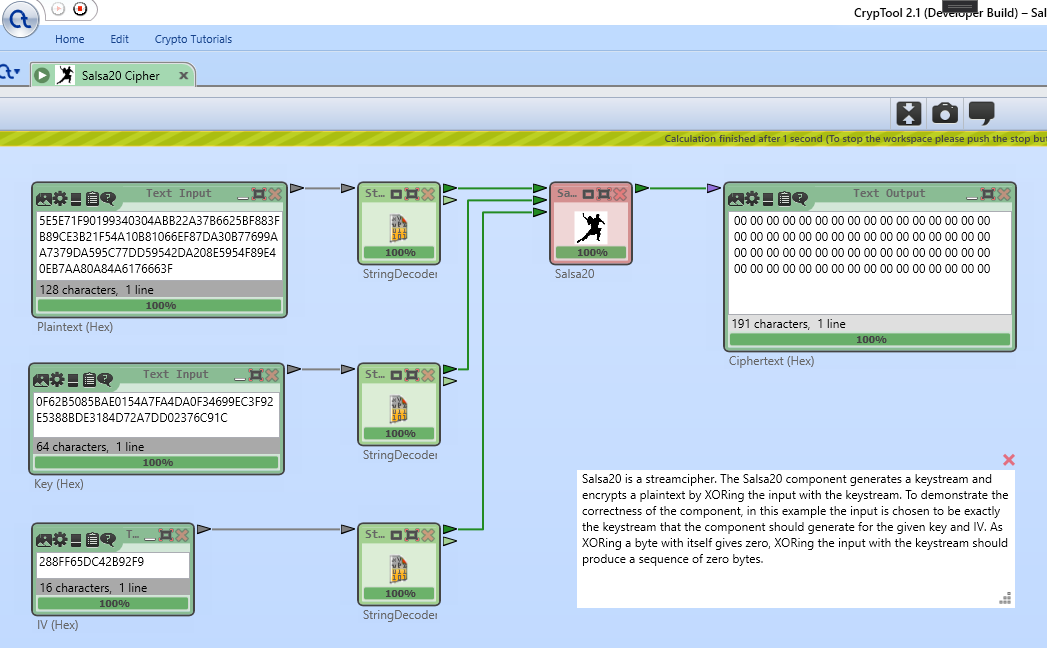
\includegraphics[width=\textwidth]{figures/ct2/salsa-crop.png}
\caption[Salsa20 CT2 template]{CT2 template for the already existing Salsa20 plugin}
\end{figure}

CrypTool 2 already has a plugin for the Salsa20 cipher but without a visualization.

During my work on the ChaCha visualization, I thought about how I could reuse my code for the ChaCha visualization to create a visualization for the Salsa20 cipher. I figured that it would not be as straight-forward as I assumed in the beginning since the visualization goes very into detail and thus the differences would involve at least different XAML code. For example, since the state is built up differently, the visualization about the state matrix initialization would need to be adapted. Also, the quarterround is slightly different which also needs to be reflected in the visualization. 

Nonetheless, I think that most of the codebase used for the ChaCha cipher could be reused to create a Salsa20 visualization, especially the navigation system and how the intermediate results are stored and retrieved for visualization. I will further discuss this in Chapter \ref{chap:futureWork}.


%%%%%%%%%%%%%%%%%%%%%%%%%%%%%%%%%%%%%%%%%%%%%%%%%%%%%%%%%%%%%%%%%%%%%%%%
\section{Other CrypTool 2 Cipher Visualizations}
\label{sec:otherCT2CipherVisualizations}

In this section, I will discuss ideas that I got from existing CrypTool 2 cipher visualizations which were also created by students during their bachelor thesis.

\subsection{AES Visualization}
\label{sec:aesVisualization}

\begin{figure}
\label{fig:aes}
\centering
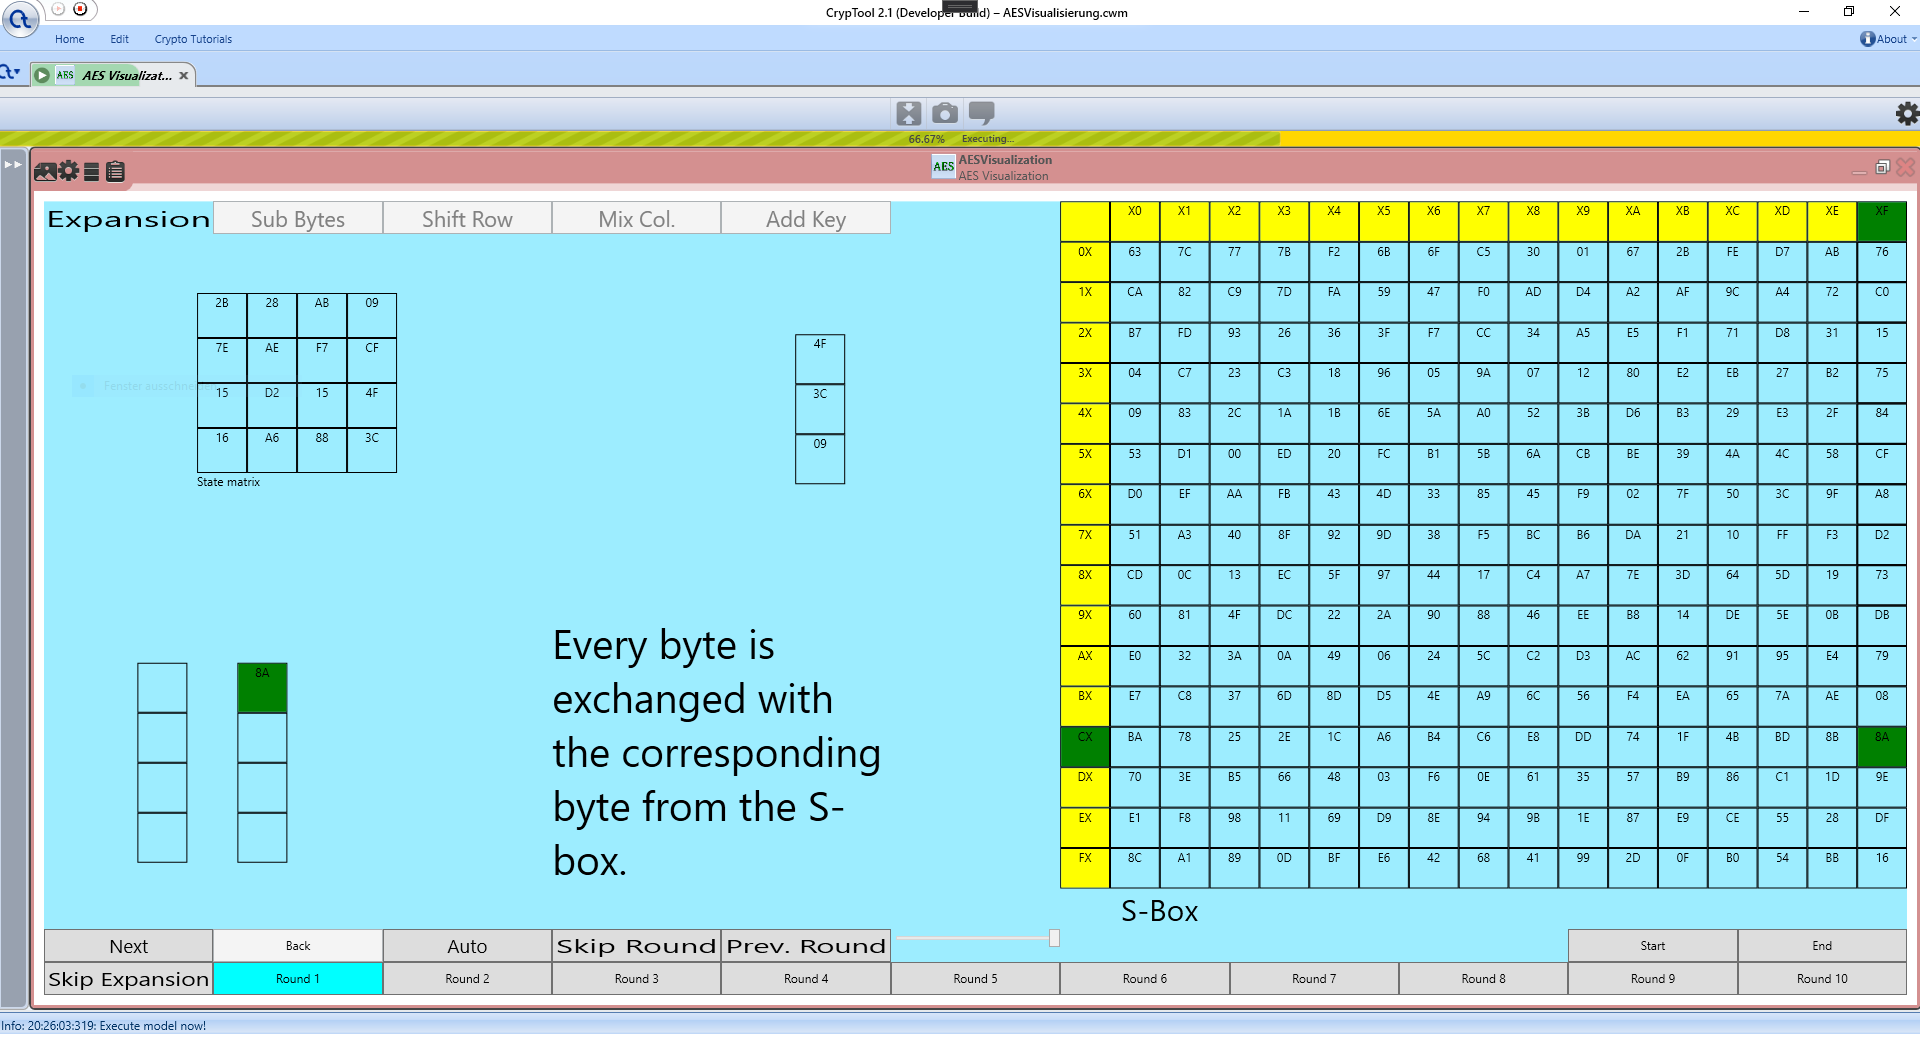
\includegraphics[width=\textwidth]{figures/ct2/aes.png}
\caption{AES visualization plugin}
\end{figure}

Matthias Becher created a visualization for the AES cipher during his bachelor thesis in 2016. It was the visualization of which I took the most inspiration for my own implementation. I also read through his bachelor thesis to see how he solved some of the problems that I encountered. For example, he wrote the following:

``The first big decision that had to be made was whether the states after each encryption operation would be calculated during the visualization or precalculated and stored at the start of the execution. One feature the plugin should have was to not only jump ahead to later operations but also to go back to previous ones. That means if the values were calculated during the visualization every time you went back they would have to be recalculated from the start. Therefore, I decided to precompute and store results of each operation in an array of byte arrays..'' \cite{aesthesis}

I came to the exact same conclusion that the values need to be precalculated for the reasons he mentioned.

Looking through his visualization, I liked how he changed the background of the elements to catch the user's attention. This is shown in Figure \ref{fig:aes}. I have used a similar mechanic during the ChaCha hash function visualization where I put a light blue background onto the state elements which will be used as the quarterround input. Also during the quarterround, I extensively used background coloring to tell the user where he should pay his attention.

Another thing I adopted from his visualization was the navigation in the top-left corner. I placed my page navigation there.

What I wanted to do differently in my navigation was to not show so many buttons all the time to the user. I was quite overwhelmed by all the buttons in the bottom navigation bar on the start even though they were disabled. Therefore, on pages which have no actions, I had no buttons in the bottom row. On pages with actions, a simple slider with a previous and next button did suffice. For the ChaCha hash function, which needed additional navigation, my navigation bar looked similar but still felt in my opinion less crowded, especially because I did not use buttons for every single round but a text input .

Further, I was confused why I could not use the ``Back'' button during the ``Expansion'' or ``Encryption'' step. For my plugin, I wanted to let the user navigate to any step in the visualization fairly simple. To achieve this, I needed to make sure that the user knows where he is and where he needs to click to go to a particular step. To give the user the information he needed, I used the dedicated page navigation in the top-left corner which stays the same on every page and tells the user on which page he currently is with bold font. Further, I numbered every single action on each page together with an action text input and how many actions a page has. The text input makes it possible for the user to immediately jump to an action.

\subsection{DES Visualization}
\label{sec:desVisualization}

\begin{figure}
\label{fig:des}
\centering
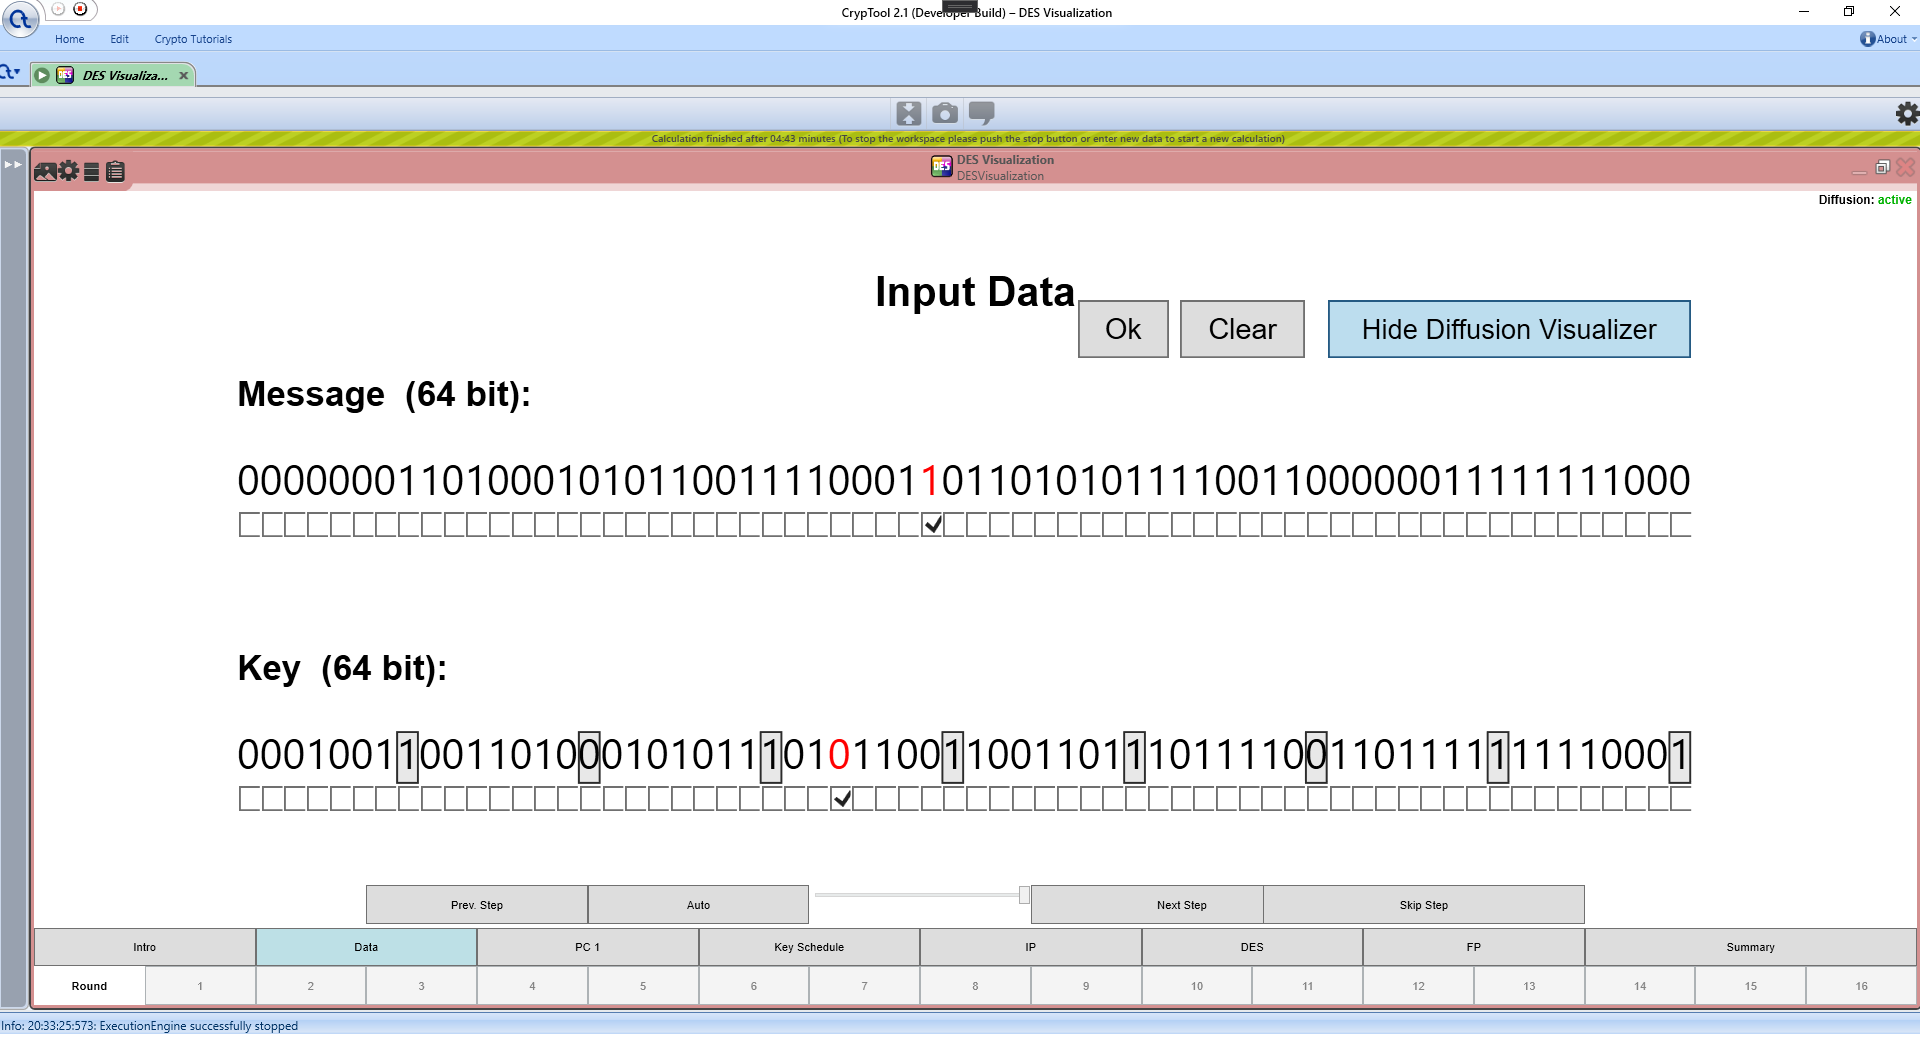
\includegraphics[width=\textwidth]{figures/ct2/des.png}
\caption{DES visualization plugin}
\end{figure}

The DES visualization was also created by a student, Lars Hoffman, for his bachelor thesis. His approach to visualizing the diffusion had the most influence on my diffusion visualization. In Figure \ref{fig:des}, you can see the page on which the user can flip bits to activate diffusion. The message and key with flipped bits will then be used to show the diffusion property of DES. 

Throughout the visualization, all values are shown in binary. This makes it possible to just mark flipped bits red since if a bit is marked red, we immediately know the value of the diffusion run (we just flip the red bit). 

I used the same coloring approach but noticed that since the ChaCha cipher was using longer keys and 512-bit blocks compared to the 64-bit blocks of DES, I needed to use hex strings for my values to save canvas space. This lead to a loss of information about the value of the diffusion run if only marking red the hexadecimal characters which are different. Therefore, I combined the usage of red color together with showing both values in two rows. In the row for the diffusion value, the difference is still marked red for easier visual recognition. This is shown in Figure \ref{fig:chachahash.mid.qr.with.diffusion}.

\subsection{Avalanche Visualization}
\label{sec:avalancheVisualization}



% !TeX spellcheck = en_GB

%%%%%%%%%%%%%%%%%%%%%%%%%%%%%%%%%%%%%%%%%%%%%%%%%%%%%%%%%%%%%%%%%%%%%%%%
\chapter{ChaCha Specification}
\label{chap:chacha}

To help with understanding the plug-in visualization and for the sake of completeness, I will summarize the specification of the ChaCha cipher in this chapter.

ChaCha is a 256-bit stream cipher based on Salsa20, both developed by Daniel J. Bernstein. It was designed to improve diffusion per round while maintaining or even increasing the performance compared to Salsa20. This makes it more secure than Salsa20 with the same amount of rounds. It was developed in the year 2008, 3 years after Salsa20 \cite{chachaspec}.

The specification can be broken apart into five main points: \\
The \textit{quarter-round} function, the \textit{little-endian} function, a hash function which utilizes the two other mentioned functions, the setup of the 512-bit state and finally, the encryption/decryption process, bringing all the individual pieces together.

I will start with the quarter round function.

\section{Quarter-round Function}
\label{sec:chacha.qr}

The ChaCha quarter-round function takes in four 32-bit unsigned integers which we will name $a$, $b$, $c$ and $d$. It also returns four 32-bit unsigned integers.\\
It modifies its input values as described in the following pseudo-code:

\begin{center}
\begin{minipage}{0.5\linewidth}
\texttt{quarterround(a,b,c,d):} \\
\hspace*{2em}\texttt{a += b; d  \^{}= a; d} \verb|<<<|\texttt{= 16} \\
\hspace*{2em}\texttt{c += d; b \^{}= c; b} \verb|<<<|\texttt{= 12} \\
\hspace*{2em}\texttt{a += b; d \^{}= a; d} \verb|<<<|\texttt{= 8} \\
\hspace*{2em}\texttt{c += d; b \^{}= c; b} \verb|<<<|\texttt{= 7} \\
\hspace*{2em}\texttt{return a, b, c, d}
\end{minipage}
\end{center}

I will call one row, consisting of one 32-bit addition, one XOR and one shift operation, a \textit{quarter-round step}. This naming convention will be reused in Section \ref{sec:userInterface}.

\section{Little-Endian Function}
\label{sec:chacha.littleendian}

The little-endian function takes in one 32-bit unsigned integer and reverses its byte order; also returning a 32-bit unsigned integer.  \\
It can be implemented as follows:

\begin{center}
\begin{minipage}{0.8\linewidth}
\texttt{littleendian(x):} \\
\hspace*{2em}\texttt{x0 = (x} \verb|>>|\texttt{ 24) \& 0xff} \\
\hspace*{2em}\texttt{x1 = (x} \verb|>>|\texttt{ 16) \& 0xff} \\
\hspace*{2em}\texttt{x2 = (x} \verb|>>|\texttt{ 8) \& 0xff} \\
\hspace*{2em}\texttt{x3 = x \& 0xff} \\
\hspace*{2em}\texttt{return (x3 } \verb|<<|\texttt{ 24) | (x2 }\verb|<<|\texttt{ 16) | (x1 }\verb|<<|\texttt{ 8) | x0}
\end{minipage}
\end{center}

\begin{remark}
Its naming has nothing to do with system endianness, but was just named like this by Bernstein for unknown reasons (most likely because reversing the byte order is what needs to be done when transmitting data between systems of different endianness).
\end{remark}

\section{ChaCha Hash Function}
\label{sec:chacha.hash}

The ChaCha hash function takes in 16 32-bit unsigned integers and returns 16 32-bit unsigned integers. The input vector $(y_0, y_1, y_2, \dots, y_{15})$ can be written as a 4$\times$4 matrix:

\begin{equation*}
\begin{pmatrix}
y_0 & y_1 & y_2 & y_3 \\
y_4 & y_5 & y_6 & y_7 \\
y_8 & y_9 & y_{10} & y_{11} \\
y_{12} & y_{13} & y_{14} & y_{15}\\
\end{pmatrix}
\end{equation*}

Using this matrix representation helps with understanding why Bernstein calls some rounds \textit{column rounds} and others \textit{diagonal rounds} in his paper (one round consists of four quarter-rounds): \\
The ChaCha hash function first iterates through all columns and then through all diagonals of the matrix; applying the quarter-round function to the four entries of each column/diagonal. After the first four quarter-rounds it therefore has changed all columns of the matrix. This is what Bernstein calls a column round in his paper. After the next four quarter-rounds, it changed all diagonals of the matrix which Bernstein analogously calls a diagonal round.

To summarize, the following quarter-rounds make up one column round:
\begin{center}
\begin{minipage}{0.5\linewidth}
\texttt{quarterround($y_0$, $y_4$, $y_8$, $y_{12}$)} \\
\texttt{quarterround($y_1$, $y_5$, $y_9$, $y_{13}$)} \\
\texttt{quarterround($y_2$, $y_6$, $y_{10}$, $y_{14}$)} \\
\texttt{quarterround($y_3$, $y_7$, $y_{11}$, $y_{15}$)} \\
\end{minipage}
\end{center}
\noindent whereas the following quarterrounds make up one diagonal round:
\begin{center}
\begin{minipage}{0.5\linewidth}
\texttt{quarterround($y_0$, $y_5$, $y_{10}$, $y_{15}$)} \\
\texttt{quarterround($y_1$, $y_6$, $y_{11}$, $y_{12}$)} \\
\texttt{quarterround($y_2$, $y_7$, $y_8$, $y_{13}$)} \\
\texttt{quarterround($y_3$, $y_4$, $y_9$, $y_{14}$)} \\
\end{minipage}
\end{center}

After a set amount of rounds (8, 12, or 20), the input vector is added to the vector on which the rounds were run. Then the byte order of each matrix entry is reversed using the little-endian function.

Having explained the basic structure of the ChaCha hash function, the following pseudo-code should complete the readers comprehension of it:

\begin{center}
\begin{minipage}{\linewidth}
\texttt{chachahash(y):} \\
\hspace*{2em}\texttt{z = copy(y)}\\
\hspace*{2em}\texttt{for(i = 0; i < ROUNDS; i += 2) \{}\\
\hspace*{4em}\texttt{// column round}\\
\hspace*{4em}\texttt{y[0], y[4], y[8], y[12] = quarterround(y[0], y[4], y[8], y[12])}\\
\hspace*{4em}\texttt{y[1], y[5], y[9], y[13] = quarterround(y[1], y[5], y[9], y[13])}\\
\hspace*{4em}\texttt{y[2], y[6], y[10], y[14] = quarterround(y[2], y[6], y[10], y[14])}\\
\hspace*{4em}\texttt{y[3], y[7], y[11], y[15] = quarterround(y[3], y[7], y[11], y[15])}\\
\hspace*{4em}\texttt{// diagonal round}\\
\hspace*{4em}\texttt{y[0], y[5], y[10], y[15] = quarterround(y[0], y[5], y[10], y[15])}\\
\hspace*{4em}\texttt{y[1], y[6], y[11], y[12] = quarterround(y[0], y[5], y[10], y[15])}\\
\hspace*{4em}\texttt{y[2], y[7], y[8], y[13] = quarterround(y[0], y[5], y[10], y[15])}\\
\hspace*{4em}\texttt{y[3], y[4], y[9], y[14] = quarterround(y[0], y[5], y[10], y[15])}\\
\hspace*{2em}\texttt{\}}\\
\hspace*{2em}\texttt{for(i = 0; i < 16; i += 1) \{}\\
\hspace*{4em}\texttt{y[i] += z[i]}\\
\hspace*{4em}\texttt{y[i] = littleendian(y[i])}\\
\hspace*{2em}\texttt{\}}\\
\hspace*{2em}\texttt{return y}
\end{minipage}
\end{center}

\section{ChaCha State Matrix}
\label{sec:chacha.matrix}

ChaCha internally uses a 512-bit state for keystream generation. The ChaCha hash function modifies this state to generate a keystream block. \\
In this section, I will explain how the state is setup which is then passed in 32-bit blocks to the ChaCha hash function.

The state is made up of a 128-bit constant, a 256-bit key section and a 128-bit nonce section. To demonstrate that the author had no hidden intent with picking his constants (nothing-up-my-sleeve number), he defined the constants to be ``expand 16-byte k'' for 128-bit keys and ``expand 32-byte k'' for 256-bit keys in ASCII.

In the 128-bit key variant, the key is concatenated with itself to create a 256-bit key. This concatenated key is then used for the state setup. If the key is already 256-bit, we do nothing and just use it as it is for the state setup.

The nonce section, which consists of a block counter and the initialization vector, is where the original version and the IETF version differ. In the original version, a 64-bit counter and a 64-bit initialization vector is used whereas the IETF version is using a 32-bit counter and a 96-bit initialization vector. \\
This means that the IETF version only partitions the nonce differently. Their reasoning to have a longer initialization vector was that with a 32-bit counter, one can encrypt messages up to 256GiB which should be enough and therefore one could make use of a bigger initialization vector. Since we need to make sure that a initialization vector is never reused with the same key, we can use a bigger initialization vector to make it more secure in cases where the same key is used by multiple senders. This is done by partitioning the 96-bit word into one 32-bit and one 64-bit section. The 32-bit section could be a unique value per sender and the last 64 bits could be a counter which is incremented for every message \cite{rfc8439}.

All state parameters are encoded by first splitting them into 32-bit chunks whose byte order is reversed except for the counter, whose byte order is first completely reversed and afterwards split into 32-bit chunks. Their 32-bit blocks are then ordered as follows to form the 512-bit state matrix:

\begin{equation*}
\begin{pmatrix}
\texttt{CONSTANT}& \texttt{CONSTANT} & \texttt{CONSTANT} & \texttt{CONSTANT} \\
\texttt{KEY} & \texttt{KEY} & \texttt{KEY} & \texttt{KEY} \\
\texttt{KEY} & \texttt{KEY} & \texttt{KEY} & \texttt{KEY} \\
\texttt{COUNTER} & \texttt{COUNTER/IV} & \texttt{IV} & \texttt{IV} \\
\end{pmatrix}
\end{equation*}

Example (all numbers are in hexadecimal with \texttt{:} as separation between bytes and already split into 32-bit chunks):\\

\begin{tabular}{ l l }
 \texttt{key (256-bit)} & \texttt{01:02:03:04 05:06:07:08 09:0a:0b:0c 0d:0e:0f:10} \\ 
 & \texttt{11:12:13:14 15:16:17:18 19:1a:1b:1c 1d:1e:1f:20}\\
 \texttt{IV} & \texttt{00:11:22:33 44:55:66:77} \\  
\texttt{Counter} & \texttt{00:00:00:00 00:00:00:01} \\
\end{tabular}
\\

\noindent Since we used a 256-bit key, we will use the ASCII constants ``expand 32-byte k''. Their byte representation is:\\

\begin{tabular}{ l l }
\texttt{Constants\phantom{MMMM}} & \texttt{65:78:70:61 6e:64:20:33 32:2d:62:79 74:65:20:6b} \\
\end{tabular}
\\

\noindent The resulting state matrix:

\begin{equation*}
\begin{pmatrix}
\texttt{61:70:78:65}& \texttt{33:20:64:6e} & \texttt{79:62:2d:32} & \texttt{6b:20:65:74} \\
\texttt{04:03:02:01} & \texttt{08:07:06:05} & \texttt{0c:0b:0a:09} & \texttt{10:0f:0e:0d} \\
\texttt{14:13:12:11} & \texttt{18:17:16:15} & \texttt{1c:1b:1a:19} & \texttt{20:1f:1e:1d} \\
\texttt{00:00:00:01} & \texttt{00:00:00:00} & \texttt{33:22:11:00} & \texttt{77:66:55:44} \\
\end{pmatrix}
\end{equation*}

\section{Encryption/Decryption}
\label{sec:chacha.encryption}

To encrypt or decrypt a input text, it is XOR'ed with the keystream. \\
To generate the keystream, the ChaCha hash function is continuously used to create 512-bit keystream blocks until we have enough to XOR every byte of the input text. The input to the ChaCha hash function is the 512-bit initial state as explained in the previous section. After each keystream block, the counter is incremented to have a different initial state as the input each time.

Since we are operating on streams, if the input message is not a multiple of 512-bit, the bits of the last block of the input message are left-aligned and the remaining bits of the keystream are dropped. This means that the output will always be the exact same length as the input.

There is no difference between encryption or decryption because XOR is the inverse to itself.

% !TeX spellcheck = en_GB

%%%%%%%%%%%%%%%%%%%%%%%%%%%%%%%%%%%%%%%%%%%%%%%%%%%%%%%%%%%%%%%%%%%%%%%%
\chapter{Plug-in}
\label{chap:Plugin}

This chapter describes the goals of the plug-in and how the implementation accommodates these goals. It also includes the thought process behind some architectural decisions that were made.\\ At the end, alternative solutions that I have taken into consideration but which were eventually abandoned are described. They complement the reasoning about the final architecture.

%%%%%%%%%%%%%%%%%%%%%%%%%%%%%%%%%%%%%%%%%%%%%%%%%%%%%%%%%%%%%%%%%%%%%%%%
\section{Goals}
\label{sec:goals}

The main goal of this plug-in was to teach students how messages are encrypted with the ChaCha cipher family. It should focus on creating an easy to understand visualization of its internals without oversimplification.\\
It should further visualize the diffusion property of the cipher on demand by making it possible for the user to alter the key, initialization vector and initial counter.\\
The plug-in should also support all variants of the cipher. This means that the user should be able to choose the key size (128-bit or 256-bit) and how often the hash function will be executed per keystream block (8, 12 or 20 rounds).\\
Since the Internet Engineering Task Force (IETF) introduced a slightly modified version of ChaCha which uses a 32-bit counter and 96-bit initialization vector, the user can also decide if he wants to use the original version by Bernstein with a 64-bit counter and 64-bit initialization vector or the one described by the IETF.

%%%%%%%%%%%%%%%%%%%%%%%%%%%%%%%%%%%%%%%%%%%%%%%%%%%%%%%%%%%%%%%%%%%%%%%%
\section{Implementation Details}
\label{sec:implementationDetails}

This section details how the goals described in the previous section were achieved. \\
In the first subsection, the key features of the plug-in are described to give a rough overview what a user can expect from the actual plug-in implementation. \\
The second subsection will then explain the user interface which is used to navigate through the plug-in and communicate to the user what is currently happening inside the cipher. \\
The last subsection then goes into technical details to explain how the plug-in internally was designed to make the user interface behave as it does.

%%%%%%%%%%%%%%%%%%%%%%%%%%%%%%%%%%%%%%%%%%%%%%%%%%%%%%%%%%%%%%%%%%%%%%%%

\subsection{Key Features}
\label{sec:keyFeatures}

\begin{figure}
\centering
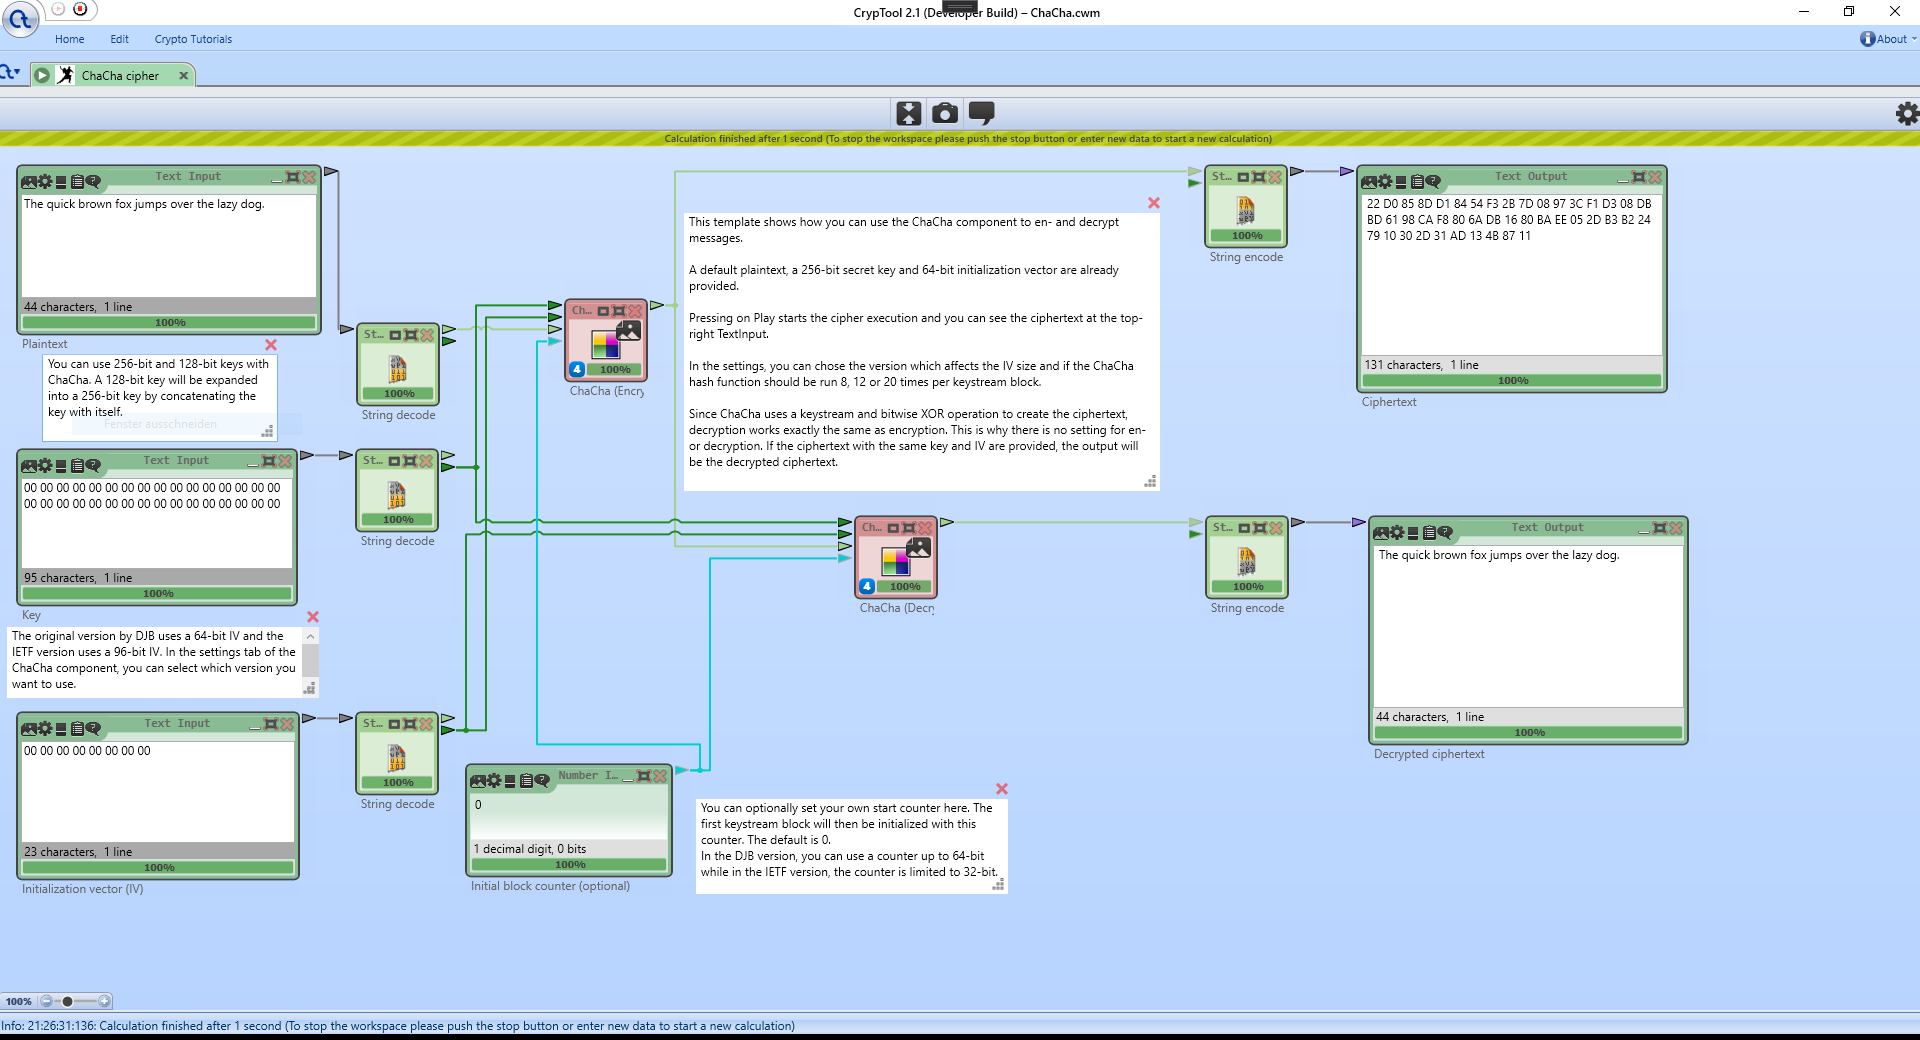
\includegraphics[width=\textwidth]{figures/ct2/plugin-template.png}
\caption[ChaCha CT2 template]{CT2 template for the ChaCha plug-in}
\label{fig:plugin.template}
\end{figure}

The plug-in offers the user the ability to input his own plaintext, key, initialization vector and initial counter using the concept of visual programming (around which CT2 is built) as one can see in Figure \ref{fig:plugin.template}. The counter is optional and defaults to zero. These values are then used to visualize the cipher execution comprehensively. Descriptions complement the visualization by providing information about what is happening. \\
As mentioned in Section \ref{sec:goals}, if the user wants to see the diffusion property of the cipher, he can alter the key, initialization vector and counter on a dedicated page inside the plug-in. \\
The version (original DJB version or IETF version) and how often the ChaCha hash function should be run per keystream block can be chosen in the plug-in settings.

\subsection{User Interface}
\label{sec:userInterface}

This subsection will describe the layout and functionality of the user interface and the reasoning behind it. First, the parts of the user interface which all pages have in common will be explained. Afterwards, we will expand upon the interface differences between the individual pages.

\subsubsection{General interface structure}

All pages have a common interface layout which consists of three sections. Each section is inside an own dedicated row.

The first section implements the navigation to move between pages. It also shows the title of the current page.

The second section shows the content of the current page. The content is not always static since it can change by using the action navigation bar in the bottom section. It includes buttons to go to the previous or next action, a slider for quicker action navigation, a text input to go to a given action and a indicator on which action the user currently is and how many actions there are in total on the current page.

I have chosen a slider over alternative solutions like individual buttons because I wanted to enable the user to quickly navigate through a page. The slider came in handy especially for the page about the ChaCha hash function where there are more than 3000 actions per keystream block. Fitting more than 3000 buttons on a single page was not feasible but would need pagination features such as showing the next set amount of buttons which would make quick navigation impossible. \\
The user can also enter a  number into the text input to the right of the slider to go to an action. But this text input is only more helpful than the slider if the user already knows the number of the action he wants to go to. If he does not, the slider creates a much better user experience. \\
If a page does not have actions, the action navigation is hidden but the space is still reserved for it to have a consistent canvas size for all pages.

I will now go into greater detail about the pages which do not have fully static content. These pages are the Diffusion page, the State Matrix Initialization page and the ChaCha Hash Function page.

\begin{figure}
\centering
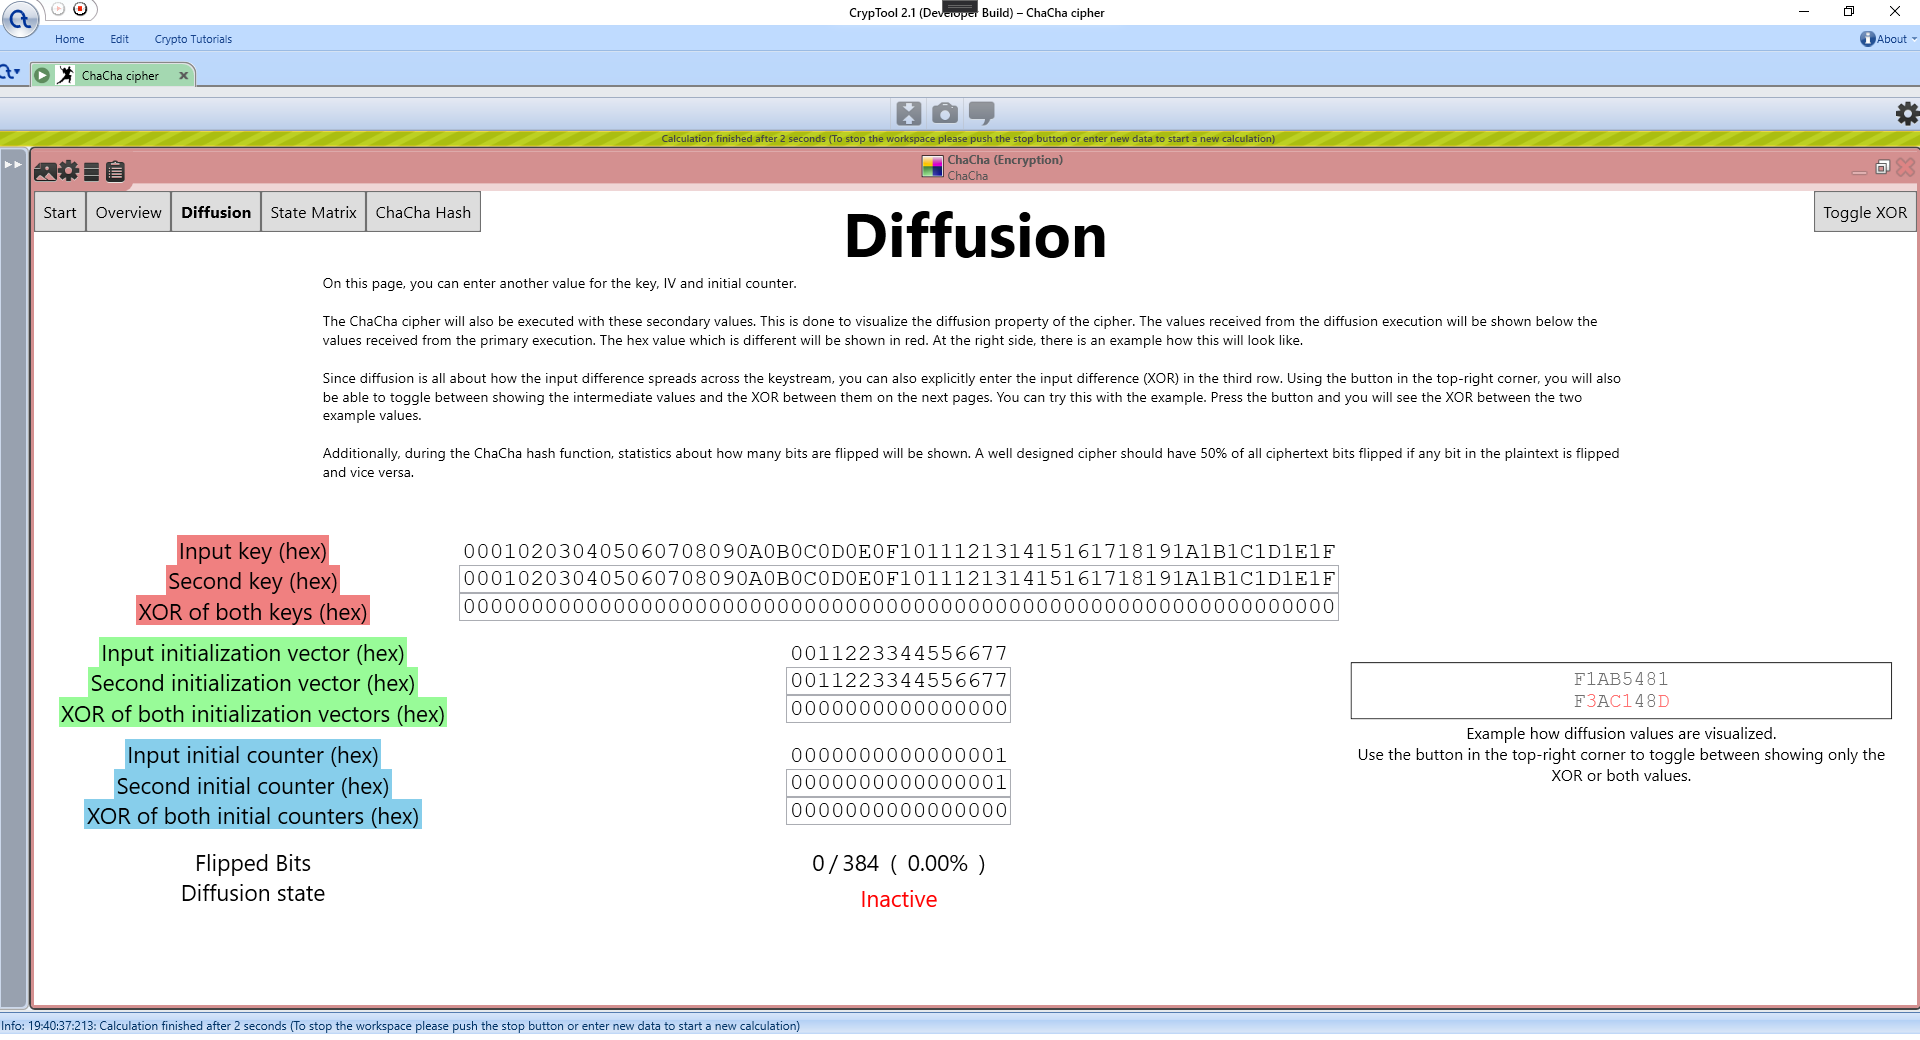
\includegraphics[width=\textwidth]{figures/ct2/all-pages/3-diffusion.png}
\caption{Diffusion page in its initial state}
\label{fig:diffusionpage}
\end{figure}

\subsubsection{Diffusion page}

As already mentioned in Section \ref{sec:keyFeatures}, on the Diffusion page (Figure \ref{fig:diffusionpage}), the user can alter the key, IV and initial counter in hexadecimal. They will be used to visualize the diffusion property. This means that during cipher execution, hexadecimal letters which are different are marked red. An example of this is shown on the Diffusion page at the right side.

I have used hexadecimal text inputs because the alternative, individual buttons for each bit, would have resulted in a lot of buttons because the key can be 256-bit. Together with the 128-bit from the counter and IV, this would have resulted in 384 individual buttons. Furthermore, clicking on individual buttons instead of entering text was more cumbersome.

Since when studying the diffusion property of a cipher, one is more interested in the difference of values (XOR) during two cipher runs instead of their actual values, the user can also explicitly input the XOR between the input value and the altered value. Additionally, if diffusion is active, the user can toggle between showing the XOR or the actual values by using the button in the top-right corner of each page.

To help with the input, the input fields show an error message if the user entered invalid characters or a too large string since the hex strings for each value must be of equal size as the input value. If the hex string is too short, it gets left-padded with zeroes to align it with the primary value.

Last but not least, the amount of flipped bits is shown in the second to last row together with a state indication in the last row if the diffusion is active or not. The diffusion is active if at least one bit was flipped. This is shown in Figure \ref{fig:diffusion.active}.

\begin{figure}
\centering
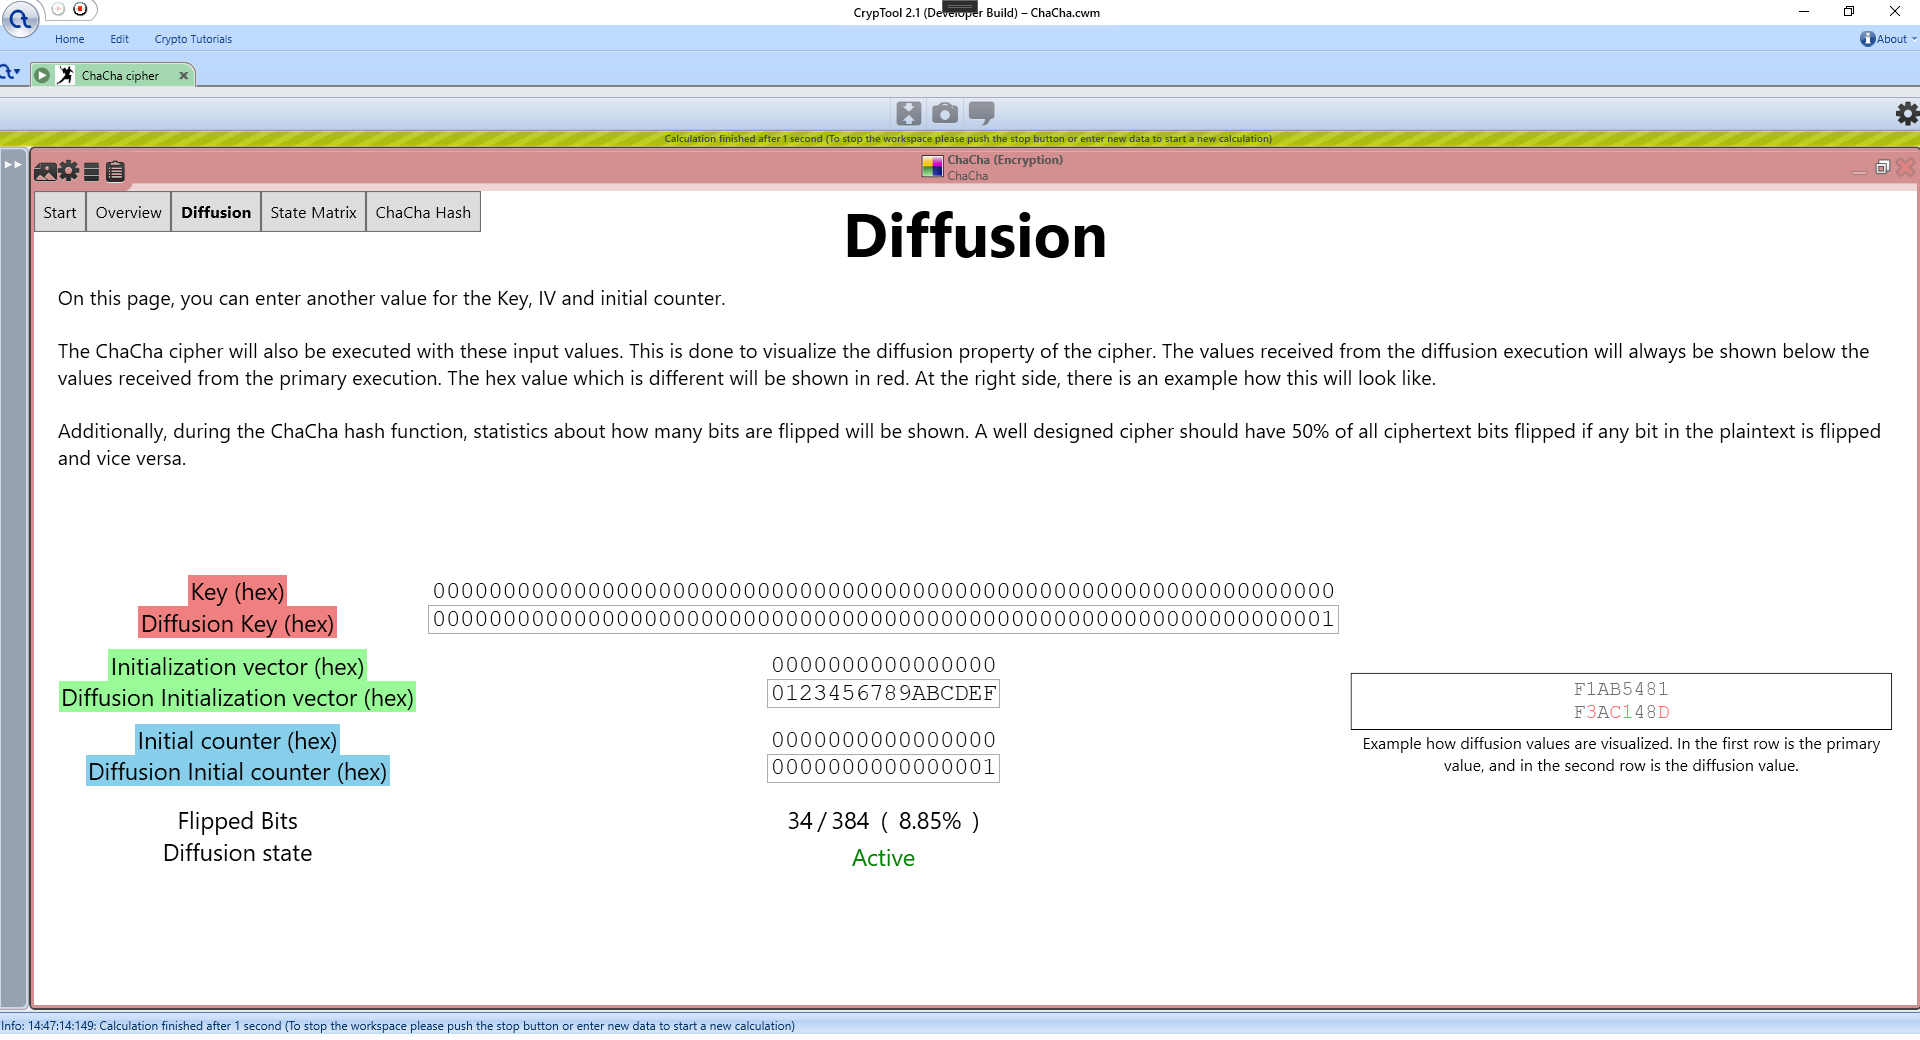
\includegraphics[width=\textwidth]{figures/ct2/diffusion/diffusion-active.png}
\caption{Diffusion page in its active state}
\label{fig:diffusion.active}
\end{figure}

\subsubsection{State Matrix Initialization page}

On the State Matrix Initialization page (Figure \ref{fig:statematrixpage}), it is shown how the initial 512-bit state for the first keystream block is build up. The generation of the next keystream blocks start with the same state but just with a different counter (as was described in Chapter \ref{chap:chacha}).

\begin{figure}
\centering
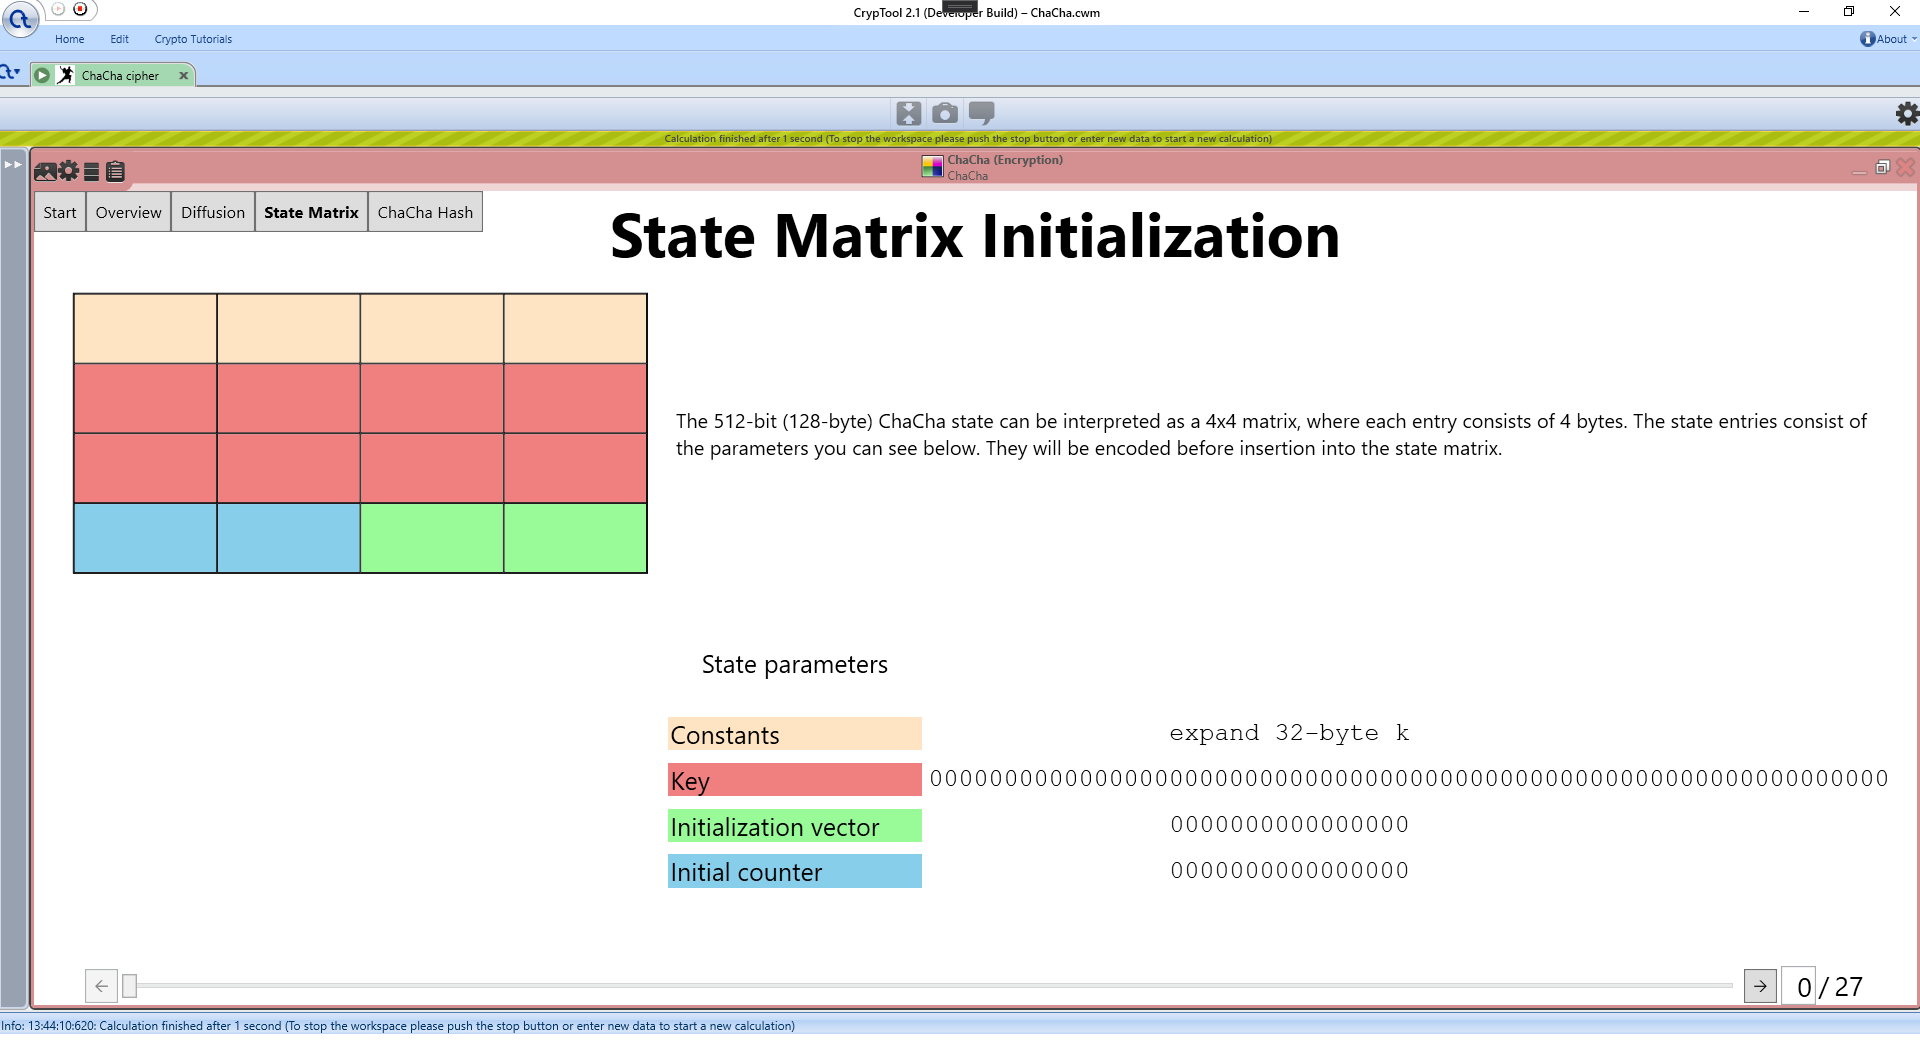
\includegraphics[width=\textwidth]{figures/ct2/all-pages/4-statematrix.png}
\caption{State Matrix Initialization page in its initial state}
\label{fig:statematrixpage}
\end{figure}

This means that only the construction of the state for the very first keystream block is shown in this page. This was done this way because I wanted to focus on one thing inside a page. I did not want to disrupt the flow of the ChaCha Hash Function page by jumping back to the visualization of the state matrix initialization just to encode a different counter. The information which is provided to the user in the first and only state matrix initialization should be enough for him to construct all following initial states without further guidance. Therefore, I focused on a comprehensive visualization of the encoding for each state parameter (constants, key, IV, counter). 

In Figure \ref{fig:statematrix.encoding}, you can see the page state during the end of each state parameter encoding. In the top-left inside each picture, you see the state. On the top-right, you see descriptions which inform the user about what the next steps are. At the bottom-left, the encoding is visualized. At the bottom-right, the state parameters with their original values before encoding are shown.

For each encoding step which corresponds to a row in the encoding section, a page action has been implemented. This means that the user can follow along each encoding step-by-step in his own speed and is not overwhelmed by a lot of information.\\
First, the constants are encoded. Since they are shown in ASCII format in the state parameters section, they are first decoded to show the actual byte values. Then the bytes are split into 4 byte chunks whose order is then reversed in the last step. \\
Afterwards, the key is encoded. It is just split into 4 byte chunks whose order is then reversed. \\
When encoding the counter, the complete byte order is first reversed, and then it is split into 4 byte chunks whose byte order is then again reversed. \\
The last parameter is the IV. It is encoded exactly the same as the key. \\

\begin{figure}
\begin{subfigure}{\textwidth}
  \centering
  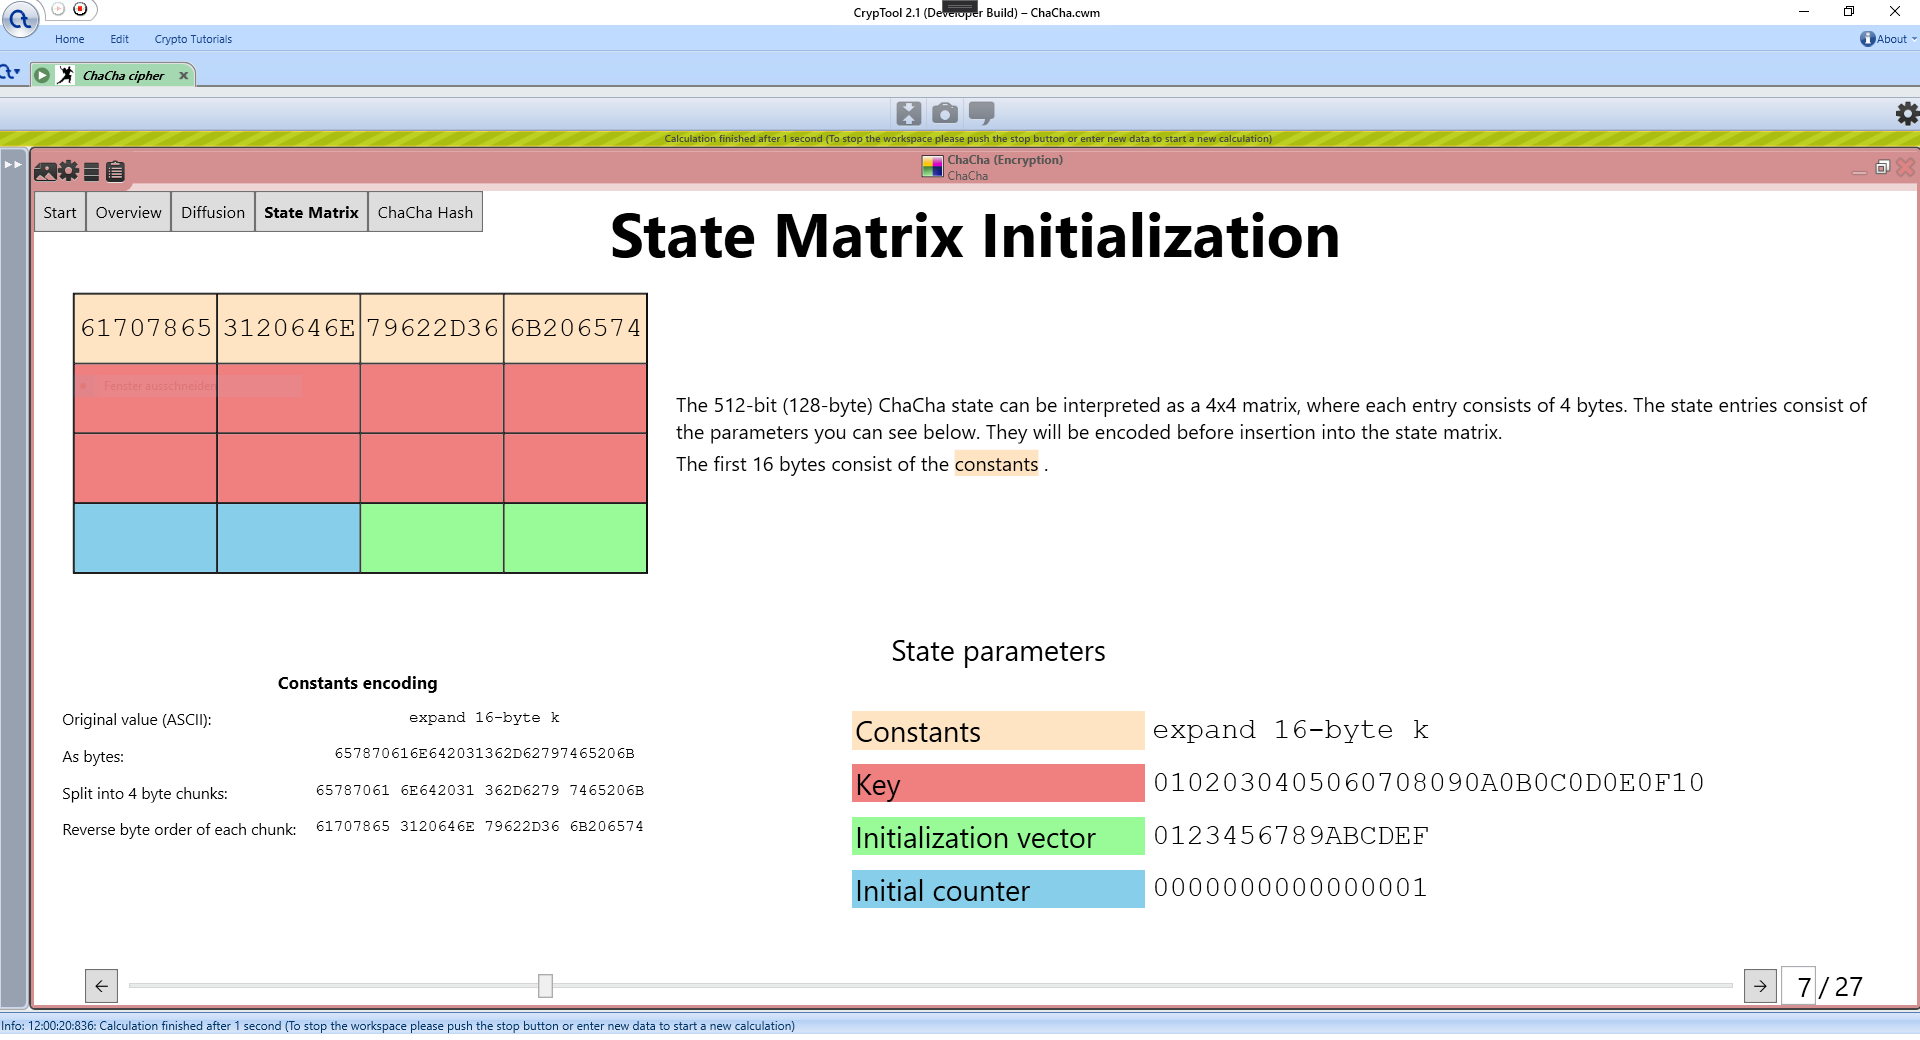
\includegraphics[width=\textwidth]{figures/ct2/state-matrix/1-state-matrix-constants.png}
  \caption{Constants encoding}
  \label{fig:statematrix.encoding.constants}
\end{subfigure}
\begin{subfigure}{\textwidth}
  \centering
  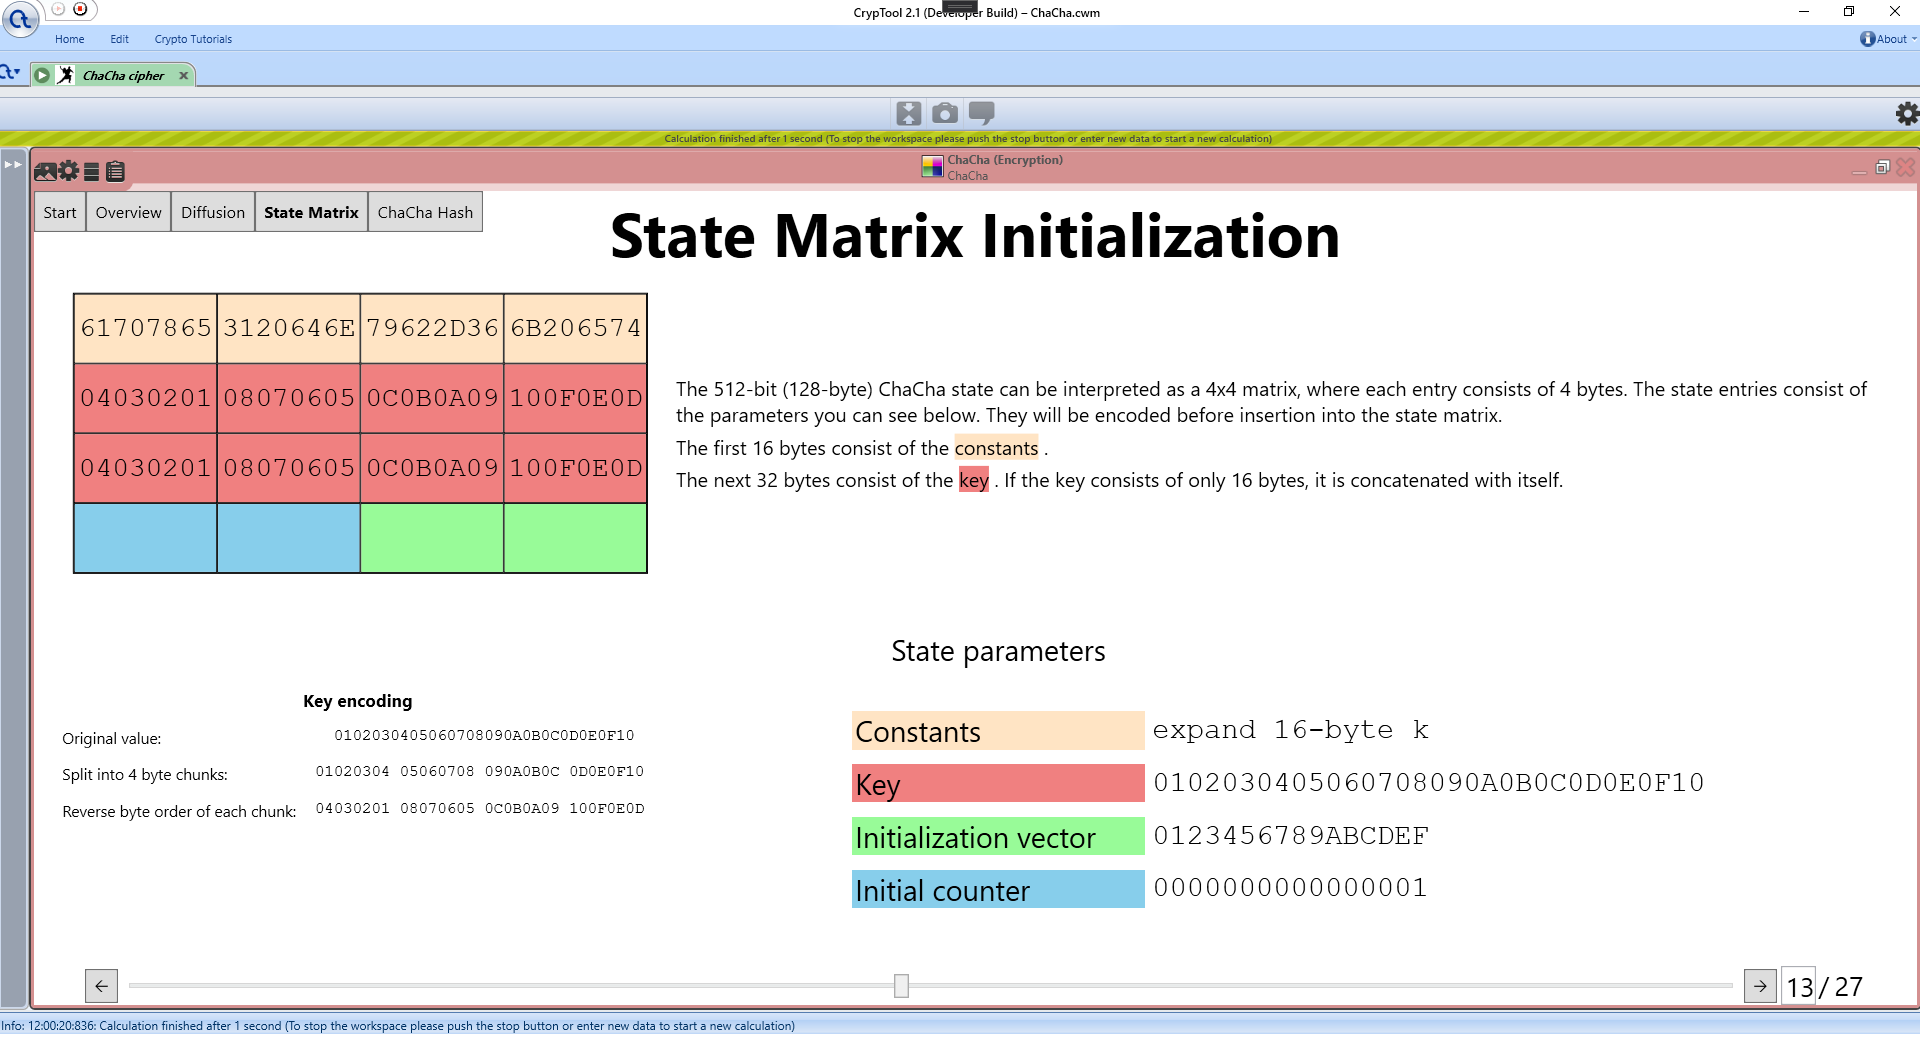
\includegraphics[width=\textwidth]{figures/ct2/state-matrix/2-state-matrix-key.png}
  \caption{Key encoding}
  \label{fig:statematrix.encoding.key}
\end{subfigure}
\end{figure}
\begin{figure}
\ContinuedFloat
\begin{subfigure}{\textwidth}
  \centering
  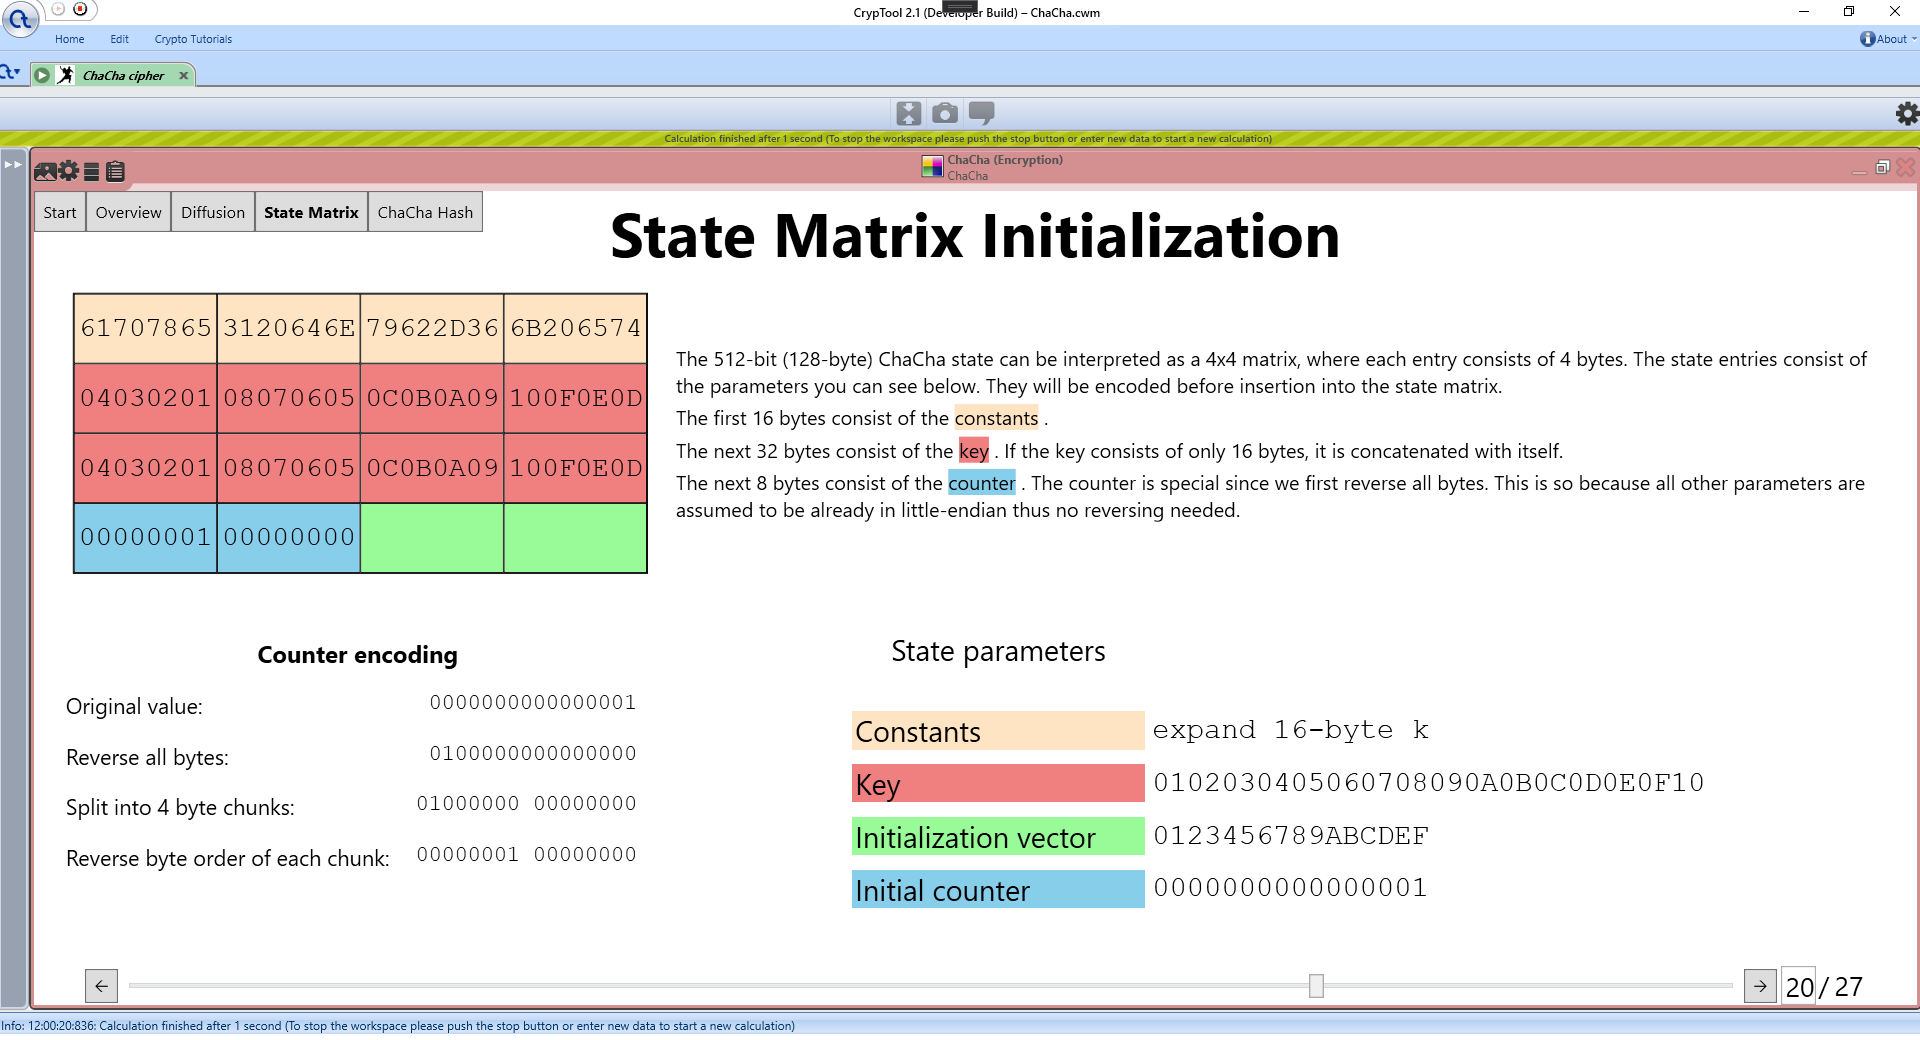
\includegraphics[width=\textwidth]{figures/ct2/state-matrix/3-state-matrix-counter.png}
  \caption{Counter encoding}
  \label{fig:statematrix.encoding.counter}
\end{subfigure}
\begin{subfigure}{\textwidth}
  \centering
  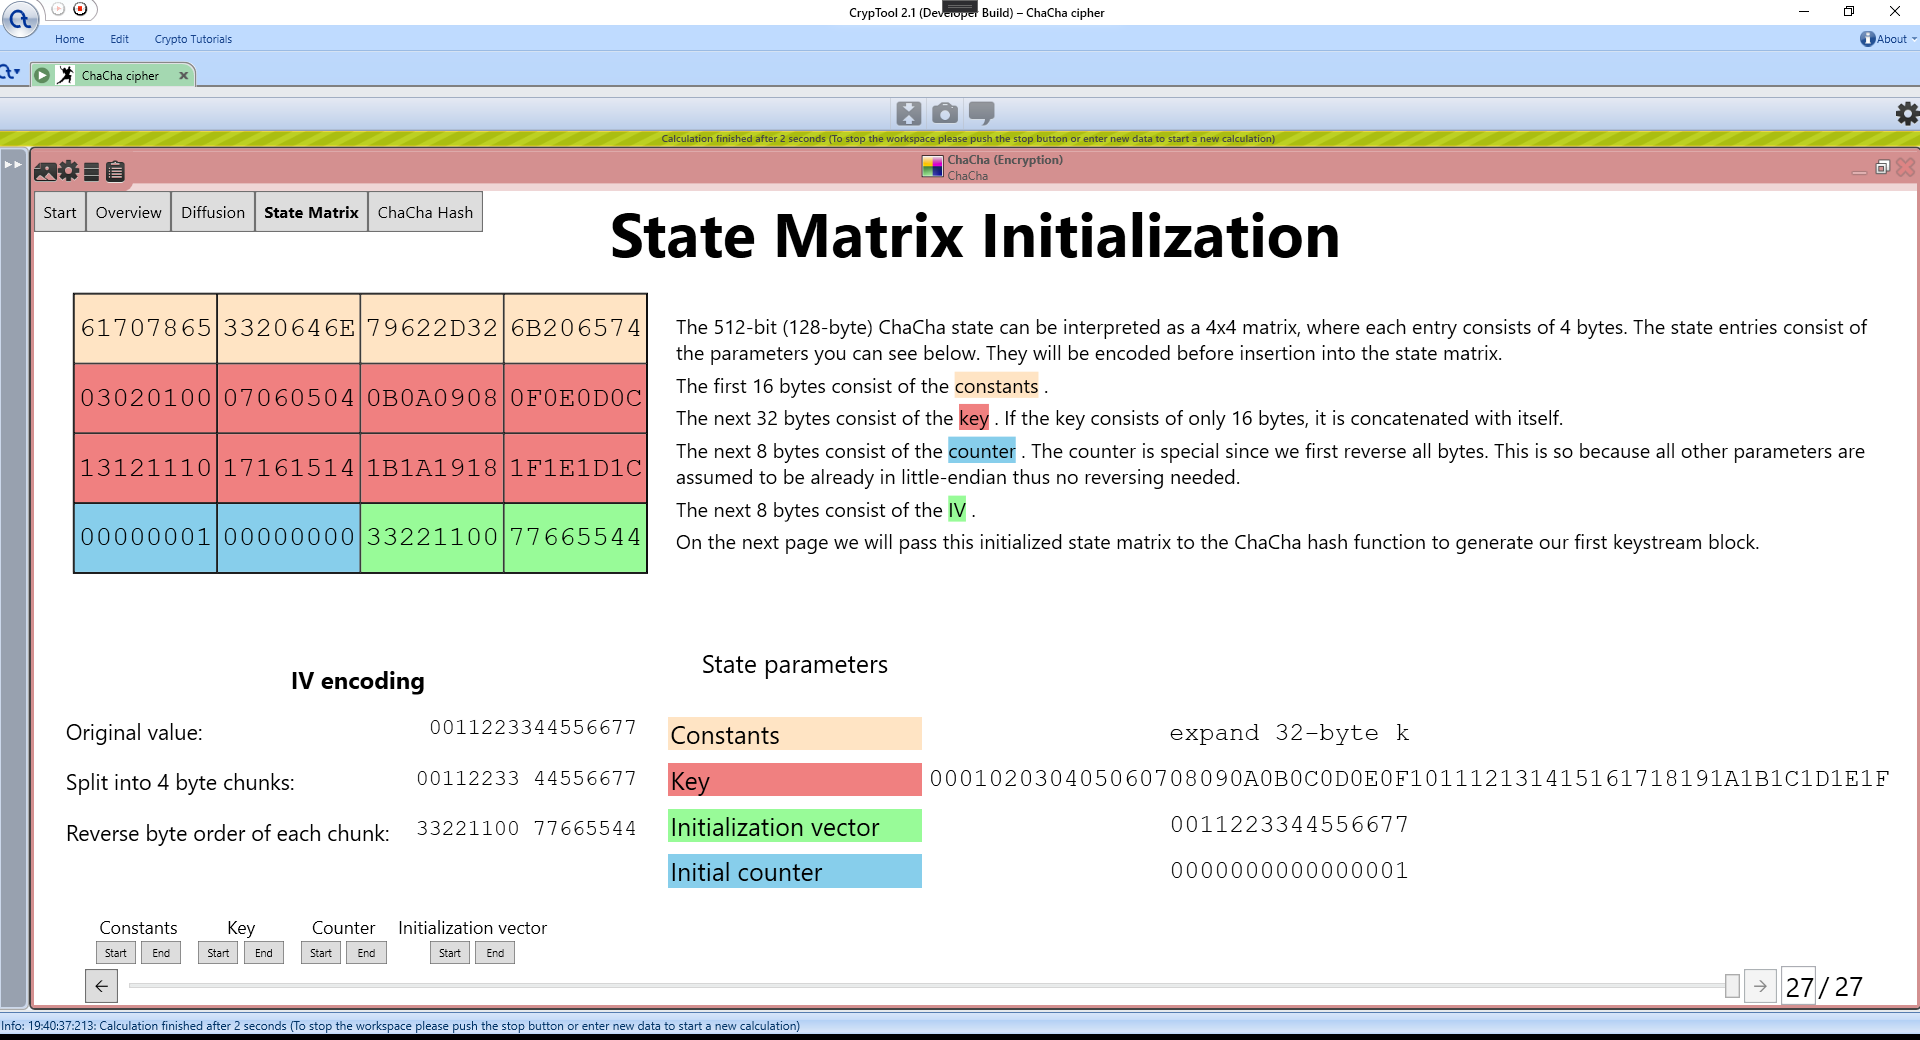
\includegraphics[width=\textwidth]{figures/ct2/state-matrix/4-state-matrix-iv.png}
  \caption{IV encoding}
  \label{fig:statematrix.encoding.iv}
\end{subfigure}
\caption[State Matrix Initialization page]{Encoding of the state parameters on the State Matrix Initialization page}
\label{fig:statematrix.encoding}
\end{figure}

\FloatBarrier

\begin{figure}[h]
\centering
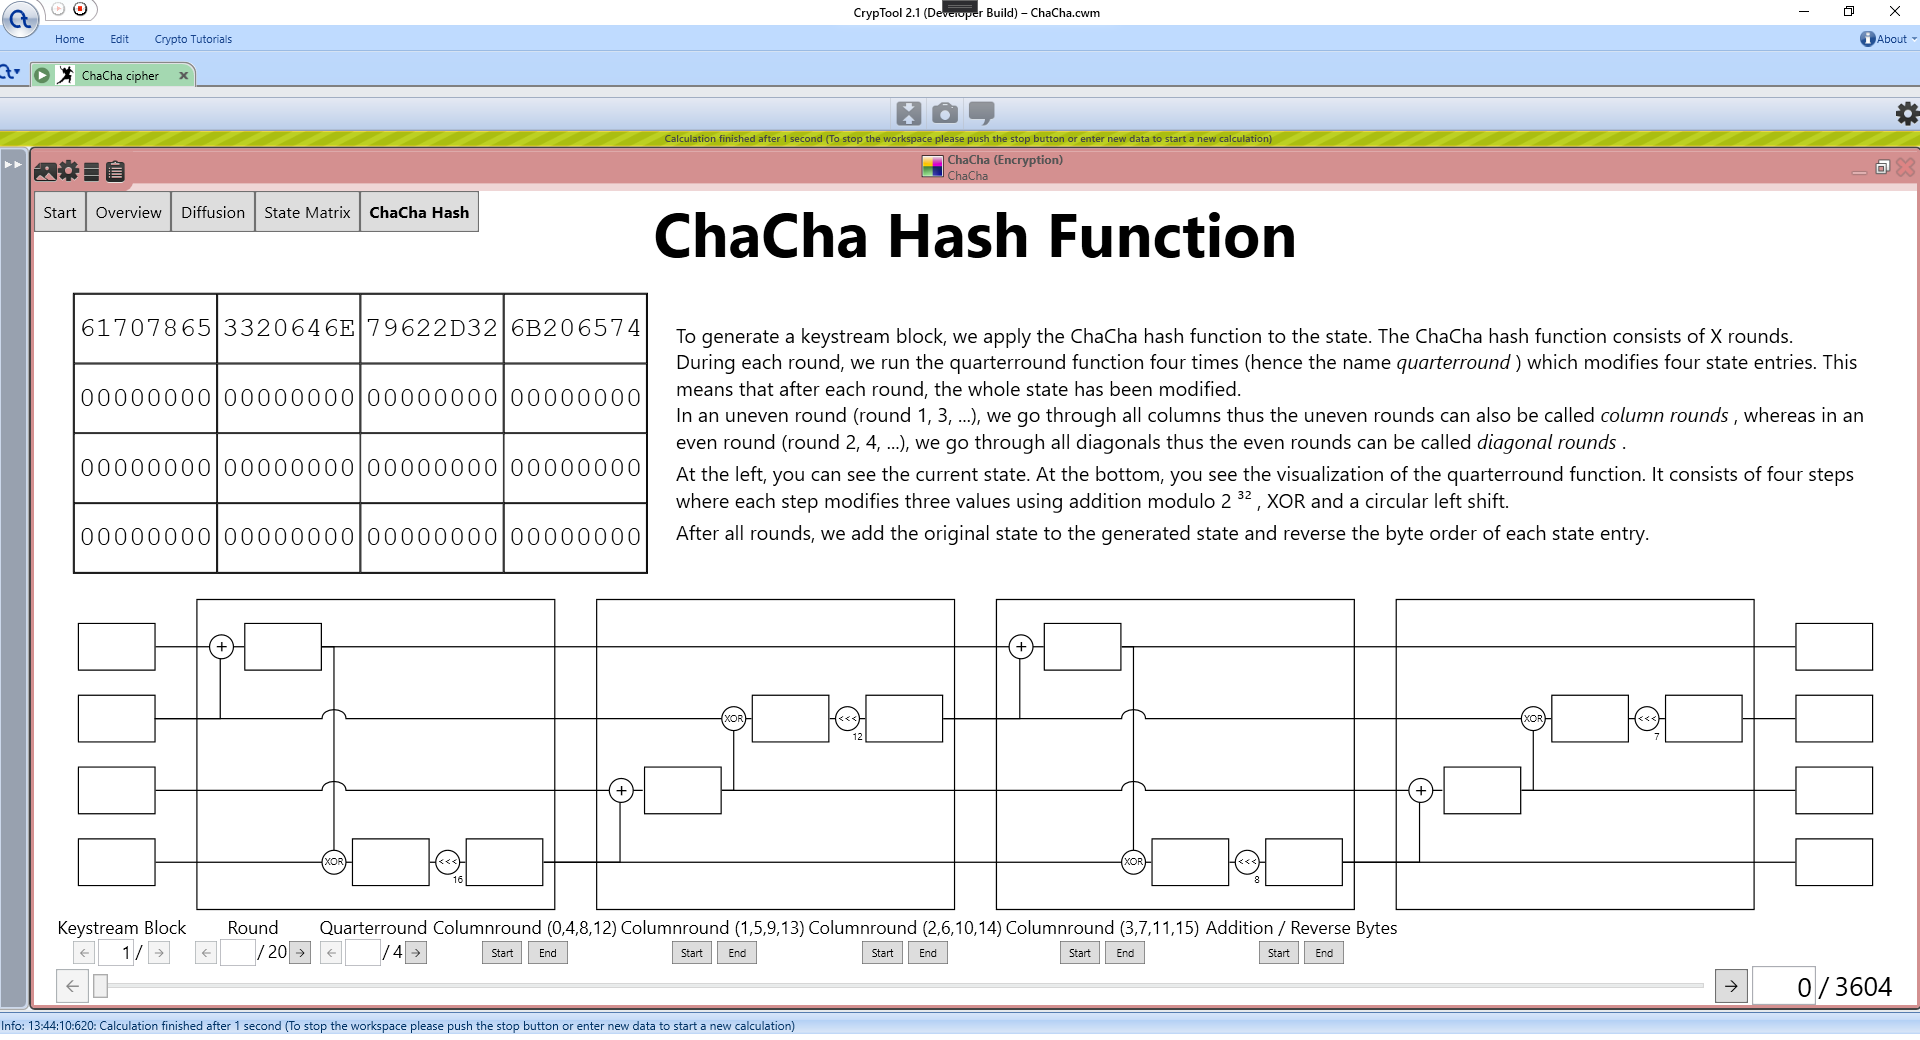
\includegraphics[width=\textwidth]{figures/ct2/all-pages/5-chachahash.png}
\caption{ChaCha Hash Function page in its initial state}
\label{fig:chachahashpage}
\end{figure}

\subsubsection{ChaCha Hash Function page}

The ChaCha Hash Function page (Figure \ref{fig:chachahashpage}) visualizes the generation of a keystream block by using two kind of visualizations: The quarter-round visualization and the addition / reverse bytes step at the end of the hash function.

\begin{figure}
  \centering
  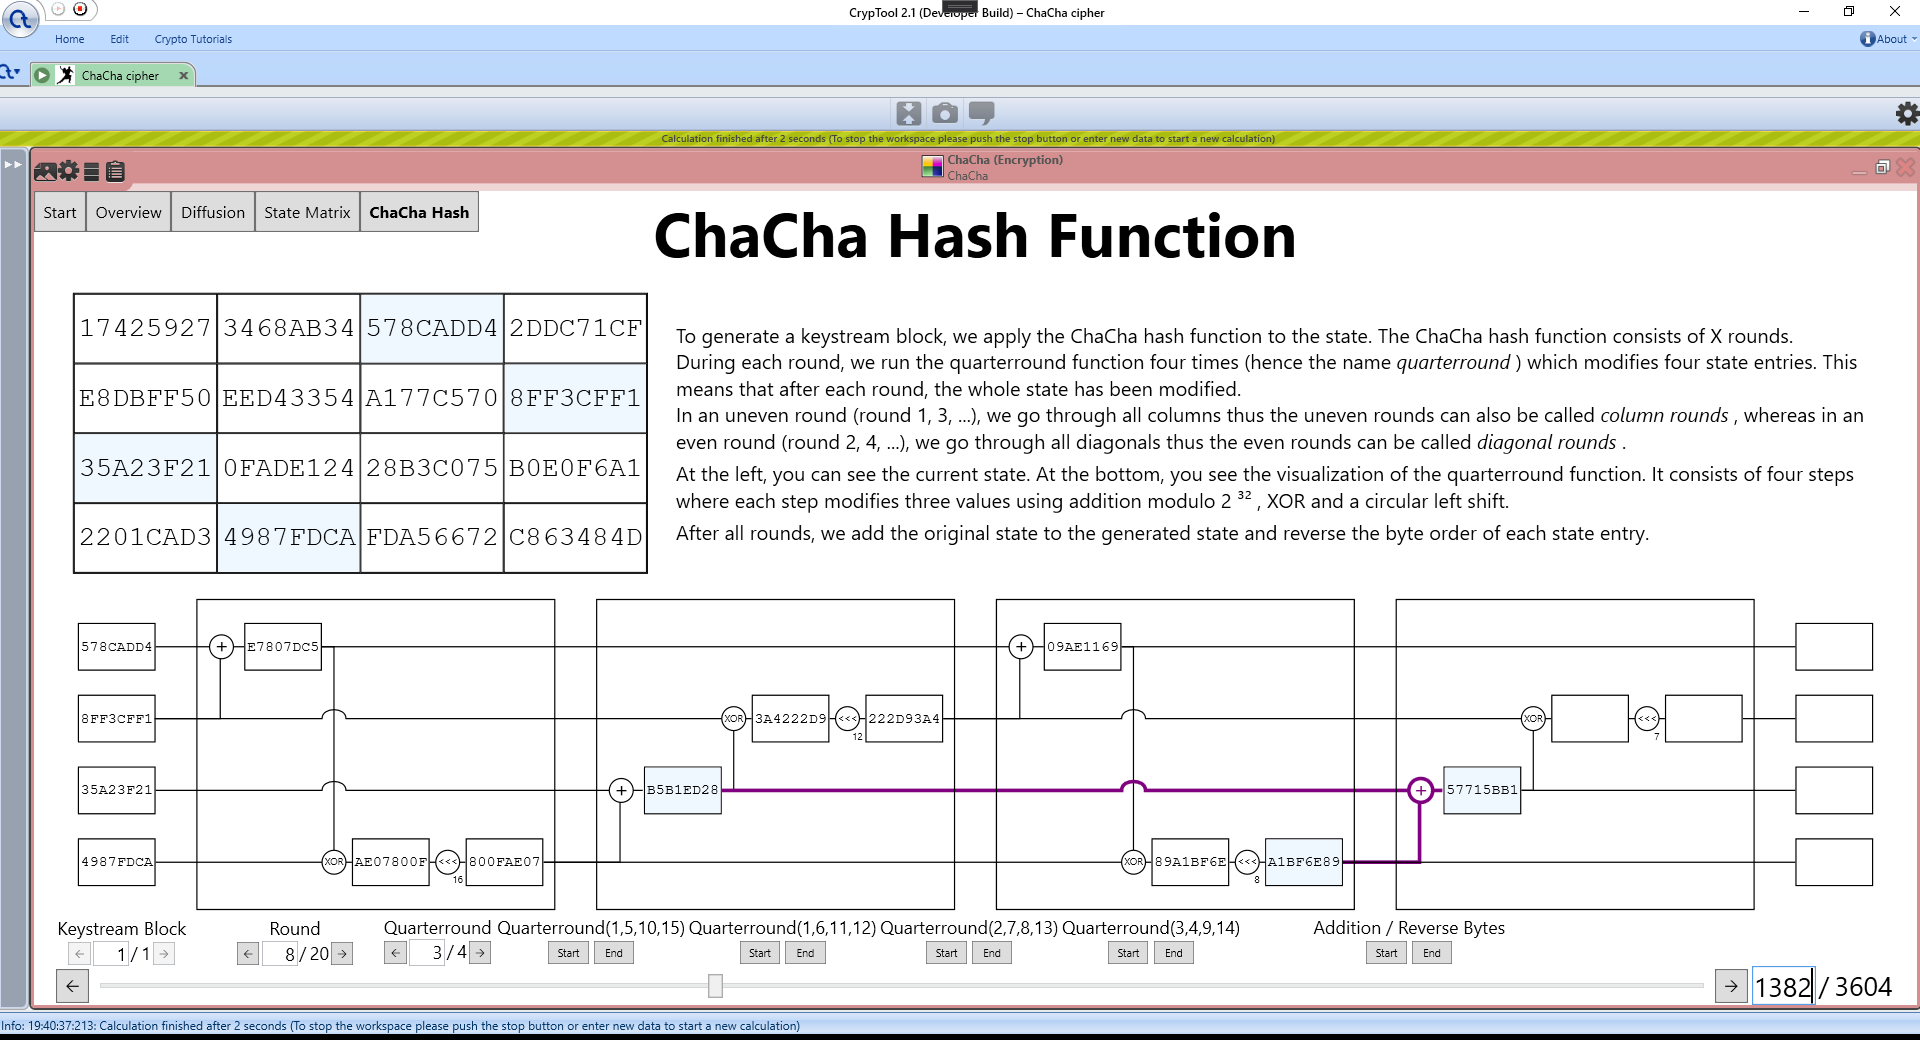
\includegraphics[width=\textwidth]{figures/ct2/chachahash/chachahash-mid-qr.png}
  \caption{Quarter-round visualization}
  \label{fig:chachahash.mid.qr}
\end{figure}

At the top of the page, you can see the current state together with a description about the ChaCha hash function.\\
At the bottom, if we are still in the ChaCha hash function loop, you can see the visualization of the quarter-rounds (Figure \ref{fig:chachahash.mid.qr}). The quarter-round visualization is split into four cells on either side and four boxes in the middle . The boxes on the two ends contain the four input and output values of the quarter-round. The boxes in the middle visualize one quarter-round step as was described in Section \ref{sec:chacha.qr}.

I have used a circuit diagram to visualize the quarter-round similar to the one found in the ChaCha section on the Wikipedia page about Salsa20 (see Figure \ref{fig:wiki.qr.circuit}). This way, I could easily show the intermediate values by putting them on the circuit lines. Furthermore, following along the visualization was very clear because all next steps are already shown just with empty values yet.

If we are finished with the loop, you can see the original state at the left, the result of adding the original state with the state after all rounds in the middle, and at the right the result of reversing the byte order of each state entry of the state in the middle (Figure \ref{fig:chachahash.end}). This is the final state and thus one 512-bit block inside the keystream with which the input message is later XOR'ed .

\begin{figure}
\centering
\begin{subfigure}[t]{0.5\textwidth}
  \centering
  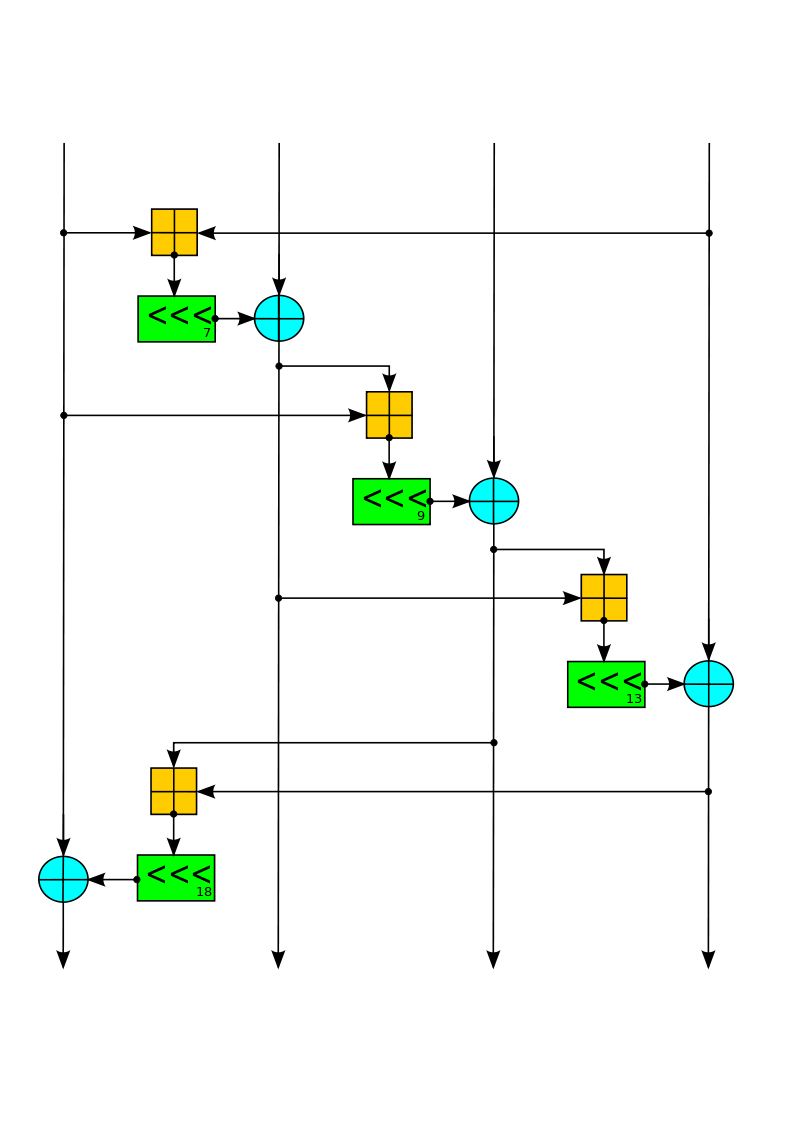
\includegraphics[width=0.99\textwidth]{figures/wiki-qr-circuit/salsa-wiki-qr-circuit.png}
  \caption{Salsa quarter-round circuit diagram}
  \label{fig:wiki.qr.circuit.salsa}
\end{subfigure}%
\begin{subfigure}[t]{0.5\textwidth}
  \centering
  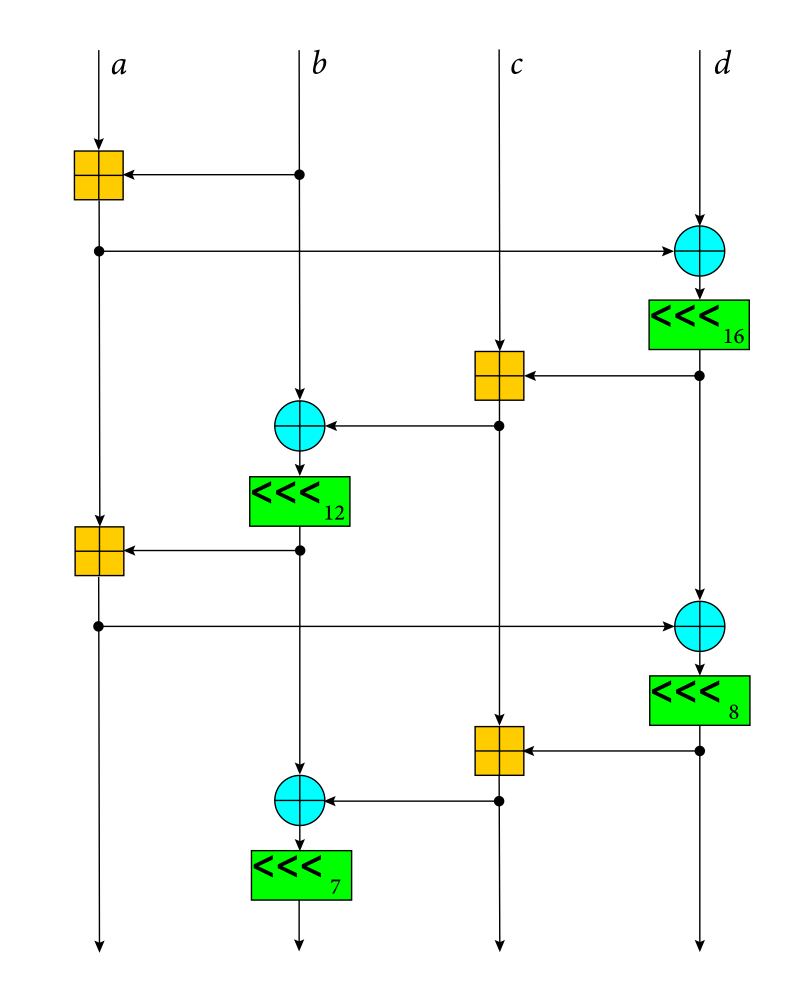
\includegraphics[width=0.99\textwidth]{figures/wiki-qr-circuit/chacha-wiki-qr-circuit.png}
  \caption{ChaCha quarter-round circuit diagram}
  \label{fig:wiki.qr.circuit.chacha}
\end{subfigure}
\caption{Quarter-round circuit diagram}
\label{fig:wiki.qr.circuit}
\centering
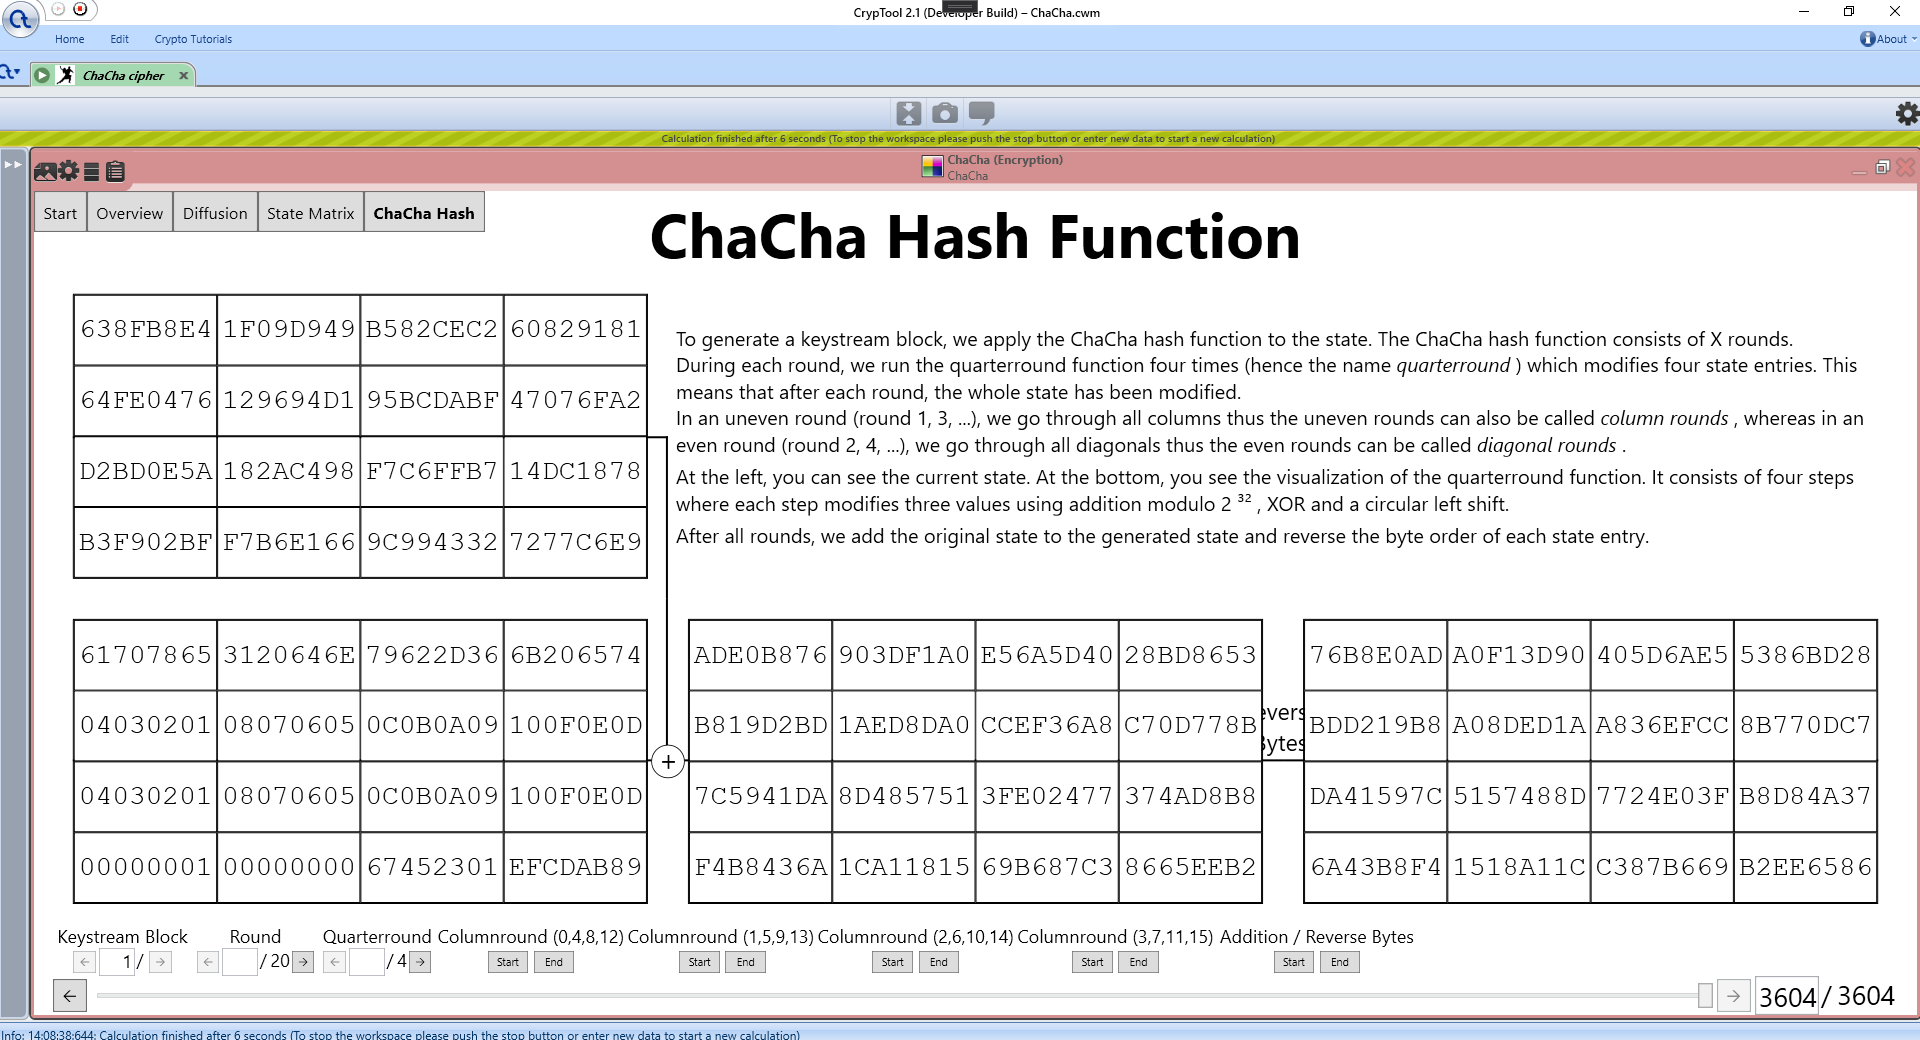
\includegraphics[width=\textwidth]{figures/ct2/chachahash/chachahash-end.png}
\caption{Addition and little-endian step visualization}
\label{fig:chachahash.end}
\end{figure}

Below the visualization and just above the slider for the page actions is another navigation bar. This helps the user to quickly navigate through the ChaCha hash function. He can use the arrow buttons to traverse through the keystream blocks, rounds or quarter-rounds or enter a number to directly go to a specific step. \\
For example, if he wants to go to the second quarter-round of the fourth round, he can enter "4" into the text input which is labelled with "Round" and press Enter or use the arrow buttons to go to the fourth round. This will take him to the start of the fourth round. He can then proceed to enter "2" into the "Quarter-round" text input. Since this will also take him to the start of the quarter-round, he can use the buttons to the right of the quarter-round input to jump to the end of specific quarter-rounds of the current round. For example, if he now wants to go to the end of the second quarter-round, he can click on "End" of the second button of the buttons which are labelled with "Quarter-round". \\
They also show the state indices in parentheses that will get updated during their quarter-round. Since column and diagonal rounds take turns, these state indices will get updated according to the current round.

Figure \ref{fig:chachahash.dr} shows exemplary how the page looks like at the end of each quarter-round of a diagonal round. As you can see, the corresponding state entry is highlighted with a light blue background. This light blue background is also used throughout the visualization to catch the user's attention about which UI elements will be updated in the next step.

Figure \ref{fig:chachahash.mid.qr.diffusion} shows the quarter-round visualization as an example how diffusion is visualized throughout the plug-in. Figure \ref{fig:chachahash.mid.qr.diffusion.both} shows the visualization with the XOR button in the top-right corner not toggled; thus showing the values from both cipher runs whereas Figure \ref{fig:chachahash.mid.qr.diffusion.xor} shows the visualization with the XOR button toggled.

\begin{figure}
\centering
\begin{subfigure}{0.5\textwidth}
  \centering
  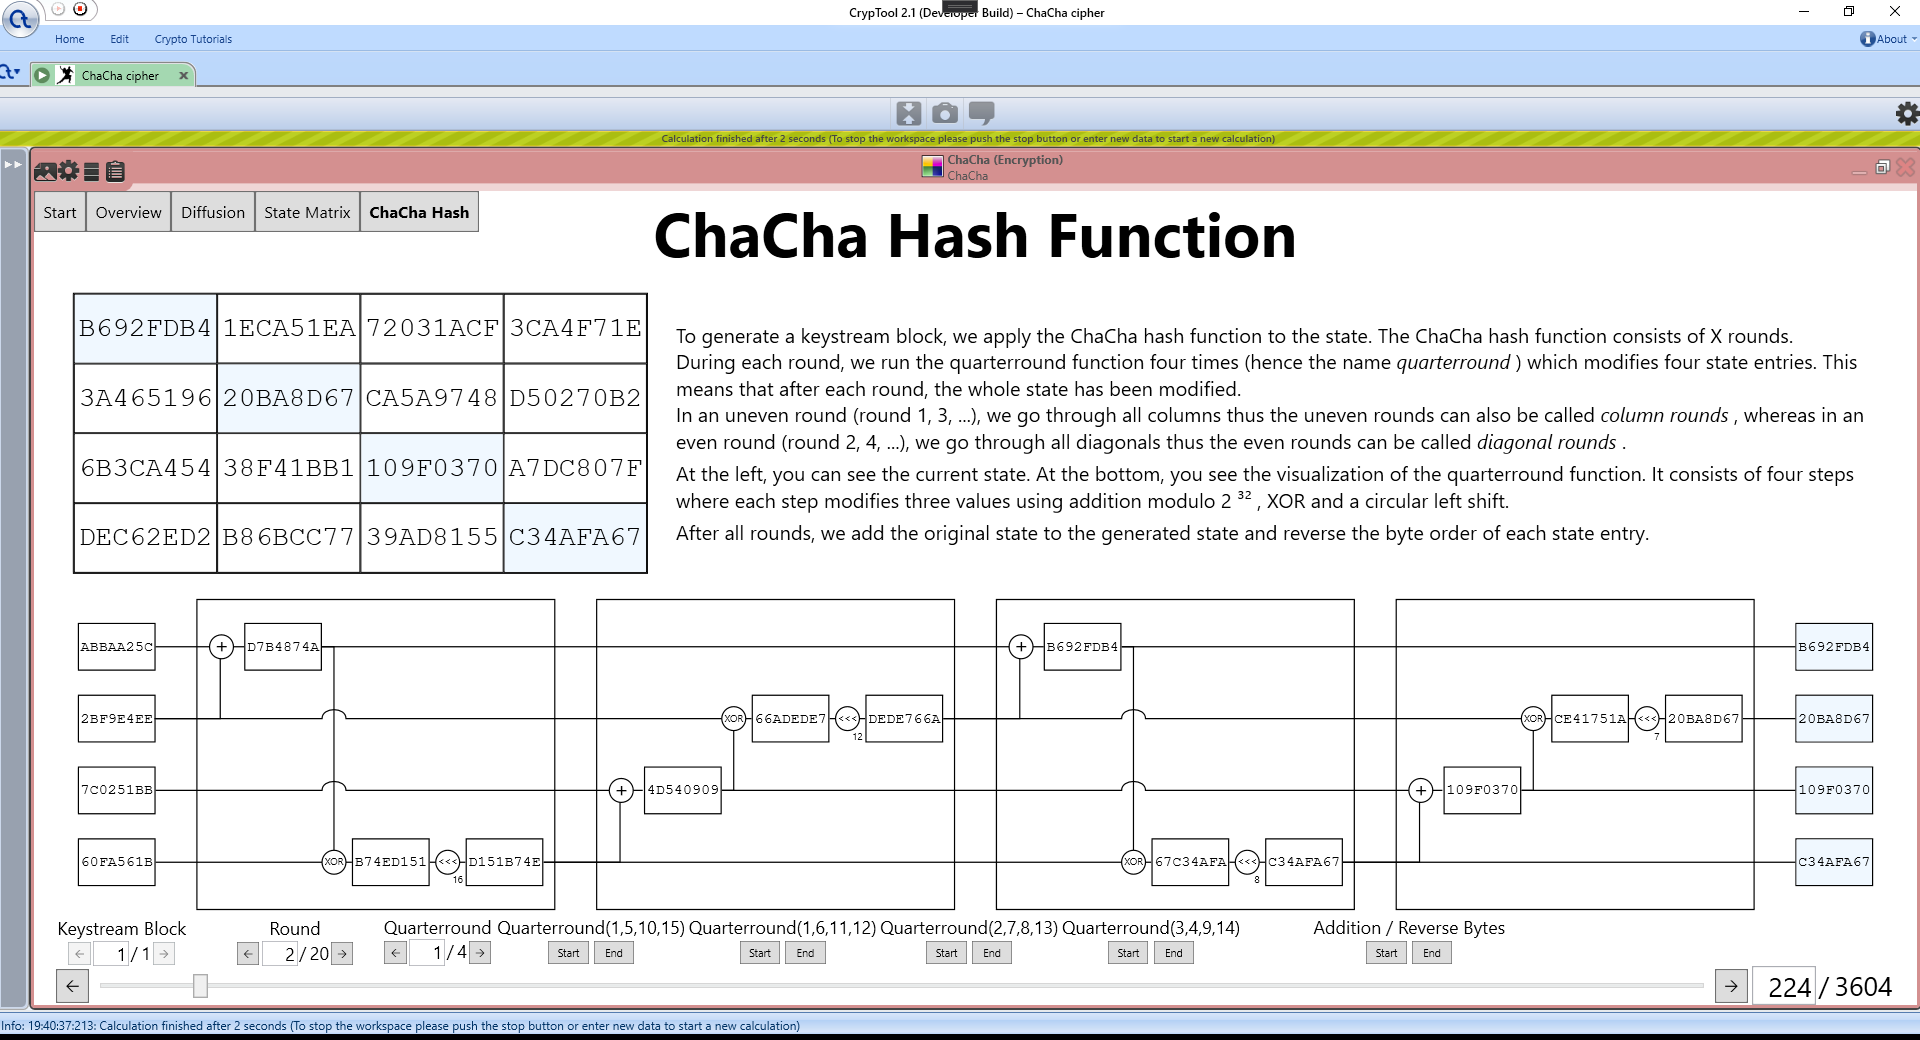
\includegraphics[width=0.99\textwidth]{figures/ct2/chachahash/chachahash-dr1-end.png}
  \caption{End of first quarter-round (diagonal round)}
  \label{fig:chachahash.dr.1}
\end{subfigure}%
\begin{subfigure}{0.5\textwidth}
  \centering
  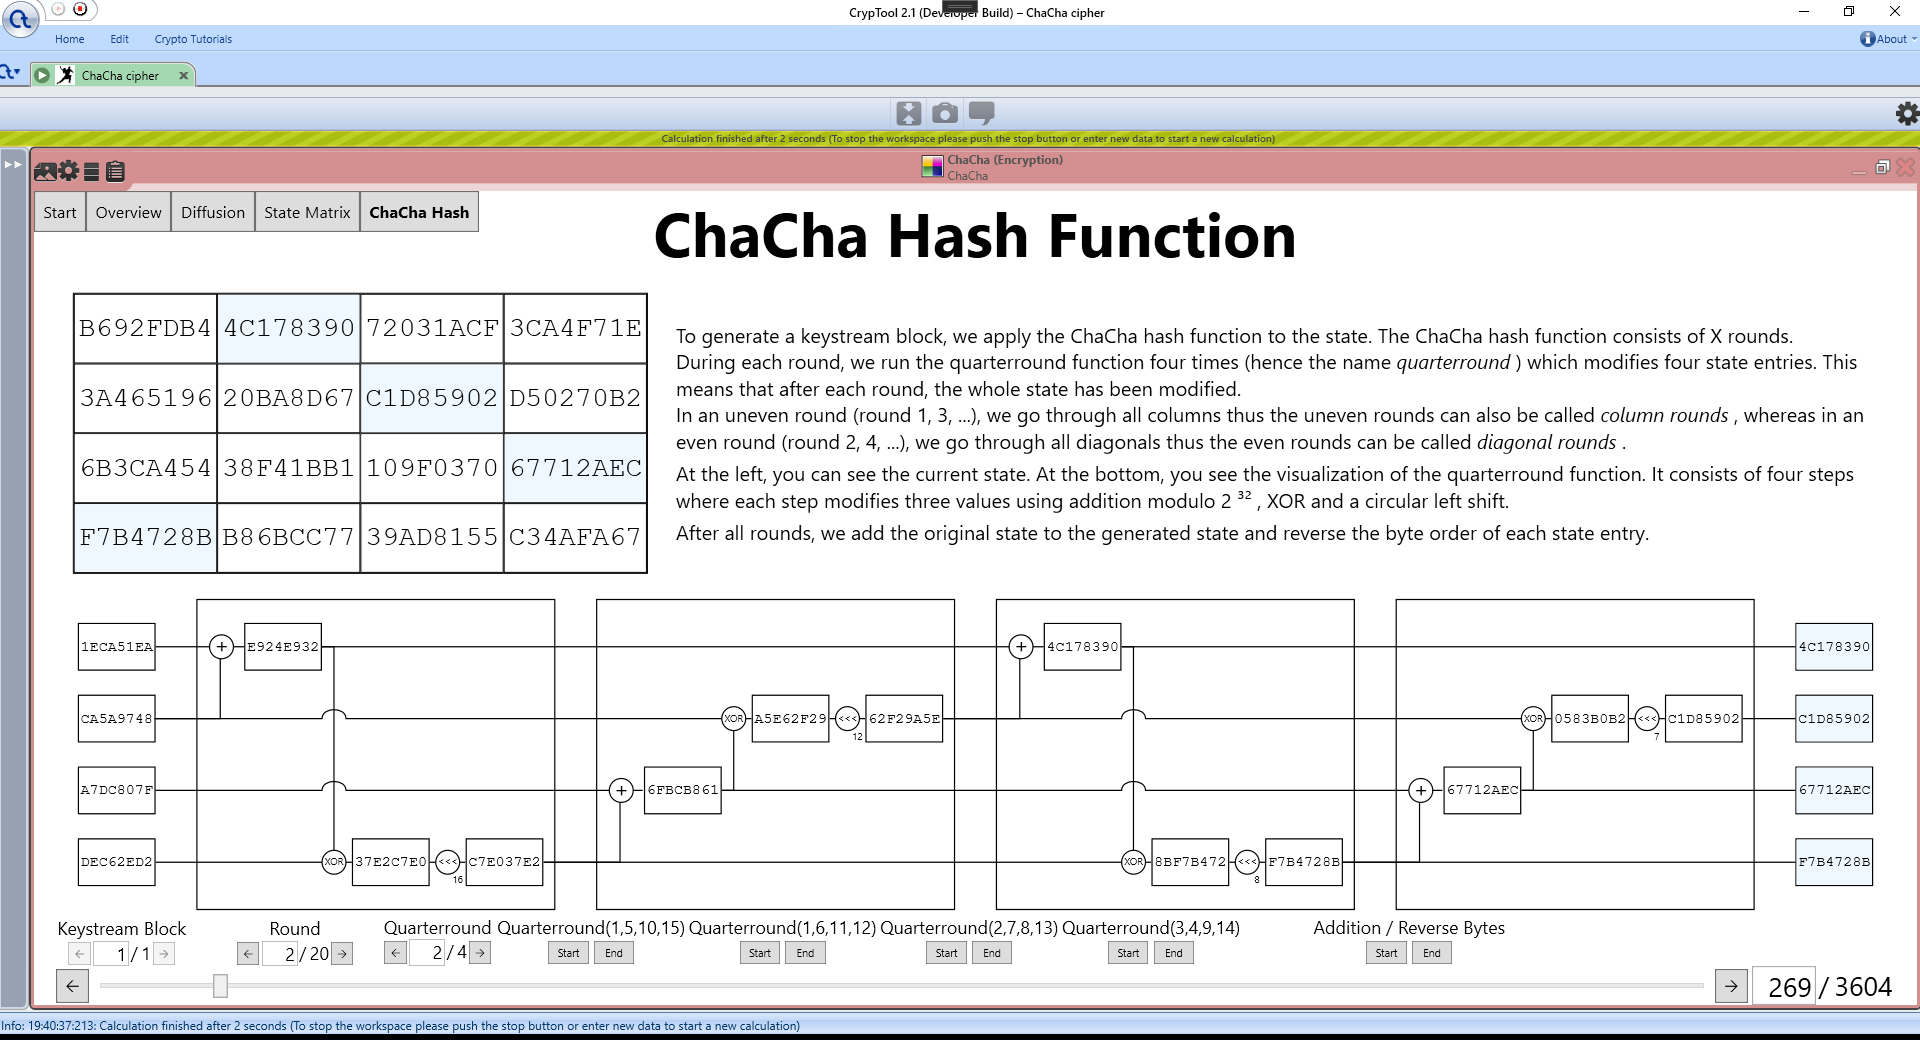
\includegraphics[width=0.99\textwidth]{figures/ct2/chachahash/chachahash-dr2-end.png}
  \caption{End of second quarter-round (diagonal round)}
  \label{fig:chachahash.dr.2}
\end{subfigure}
\begin{subfigure}{0.5\textwidth}
  \centering
  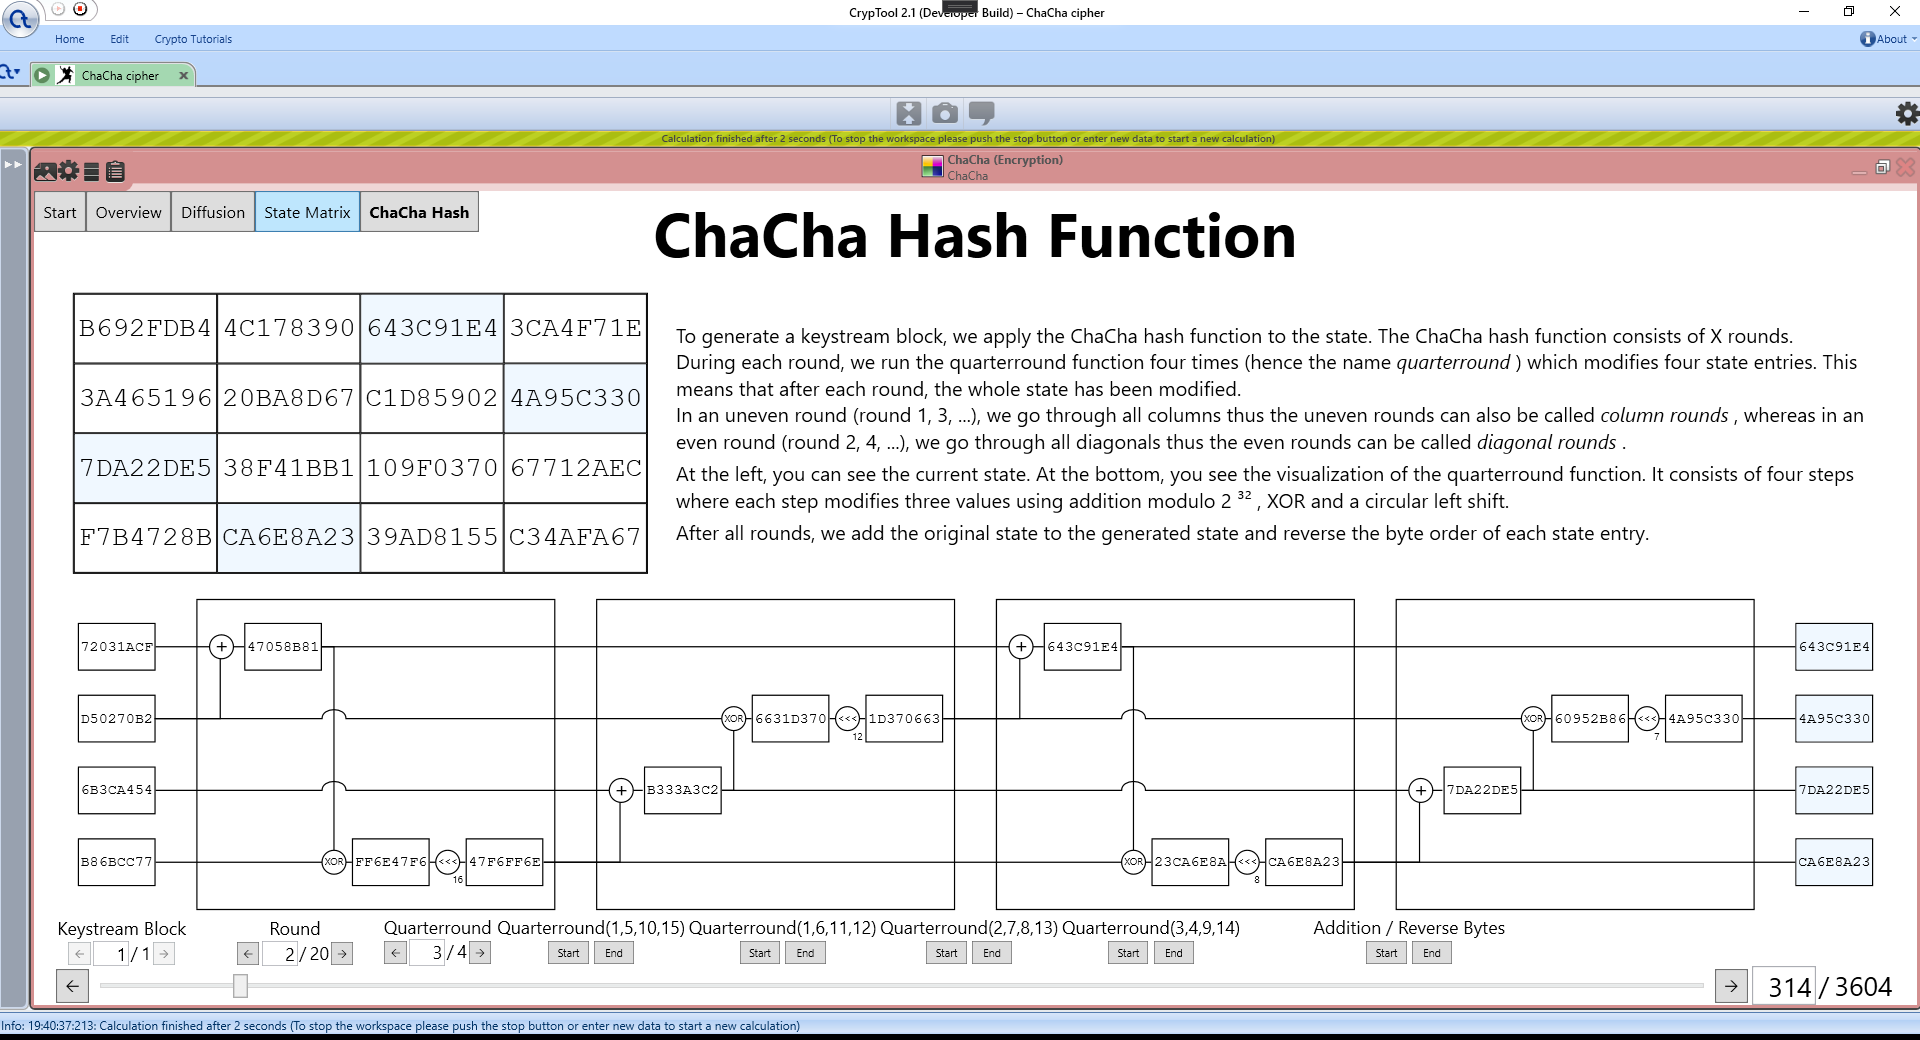
\includegraphics[width=0.99\textwidth]{figures/ct2/chachahash/chachahash-dr3-end.png}
  \caption{End of third quarter-round (diagonal round)}
  \label{fig:chachahash.dr.3}
\end{subfigure}%
\begin{subfigure}{0.5\textwidth}
  \centering
  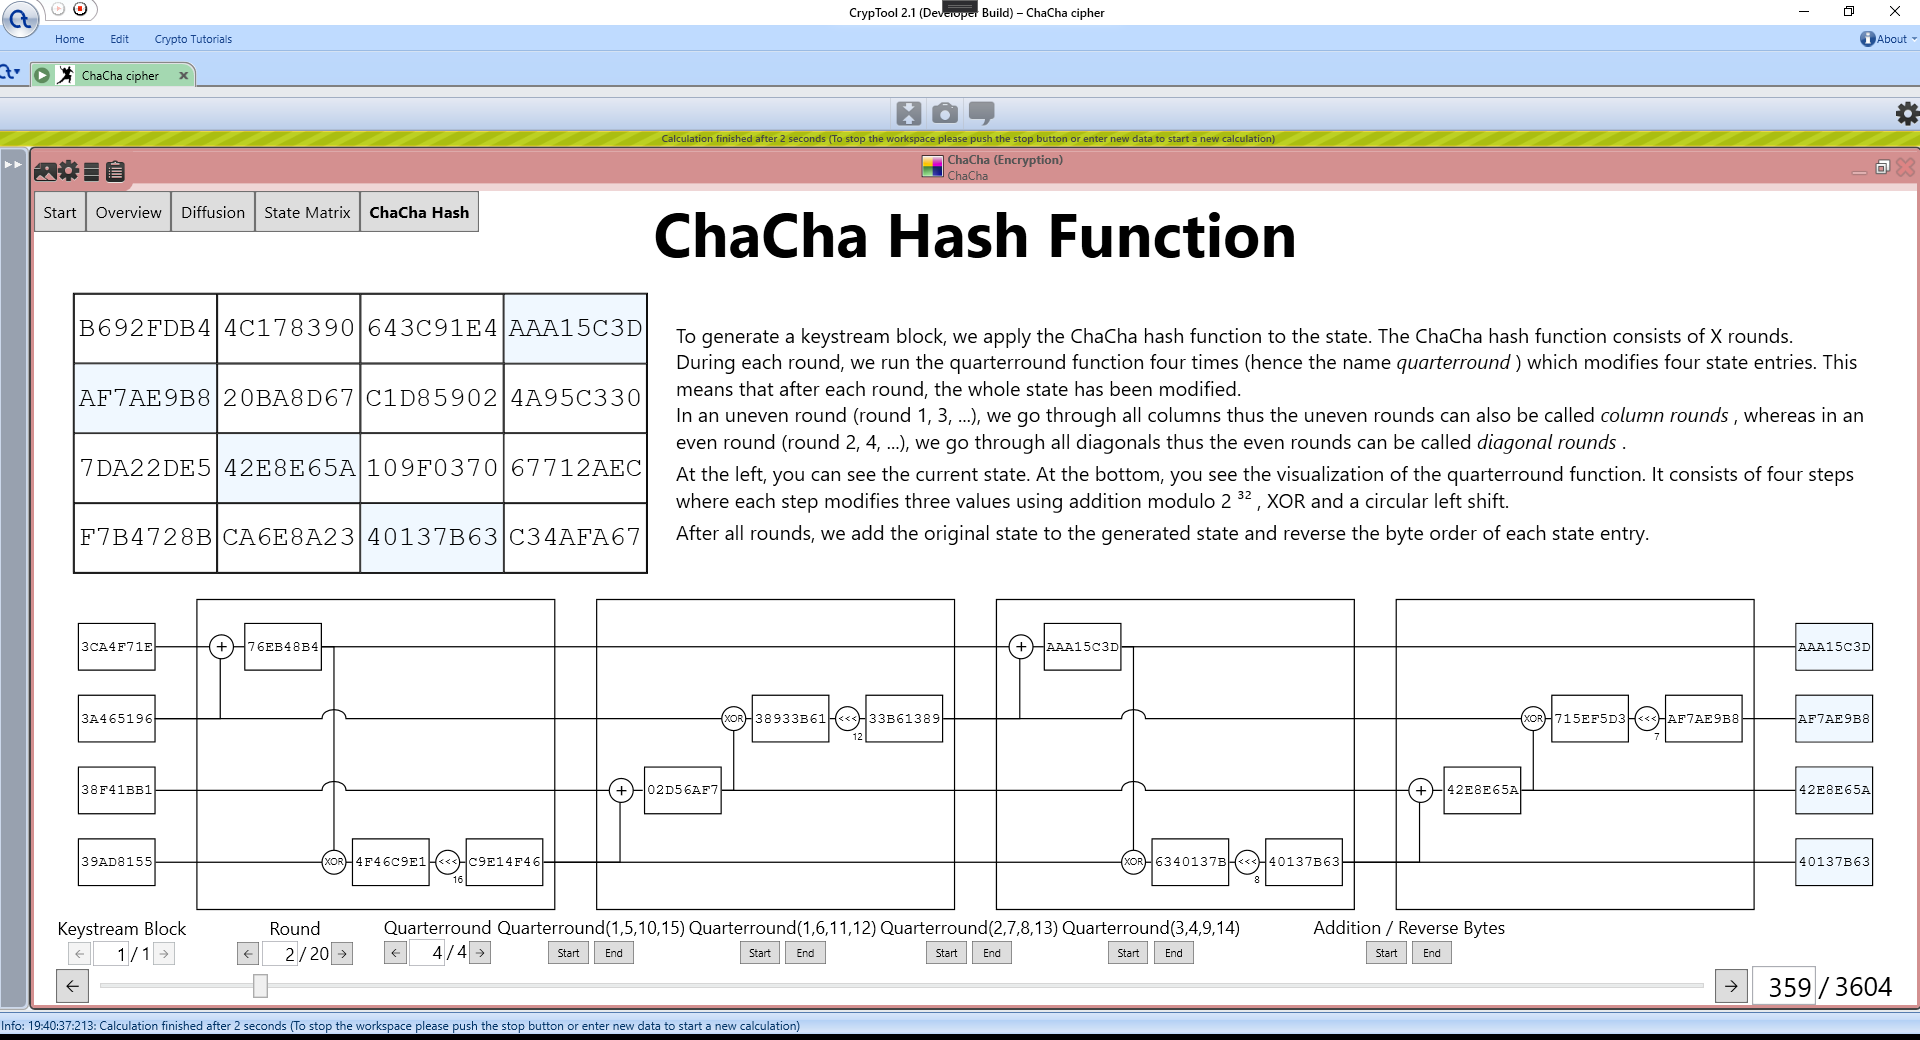
\includegraphics[width=0.99\textwidth]{figures/ct2/chachahash/chachahash-dr4-end.png}
  \caption{End of fourth quarter-round (diagonal round)}
  \label{fig:chachahash.dr.4}
\end{subfigure}
\caption[End of diagonal rounds]{End of each quarterround execution of a diagonal round}
\label{fig:chachahash.dr}
\end{figure}

\begin{figure}
\begin{subfigure}[t]{\textwidth}
  \centering
  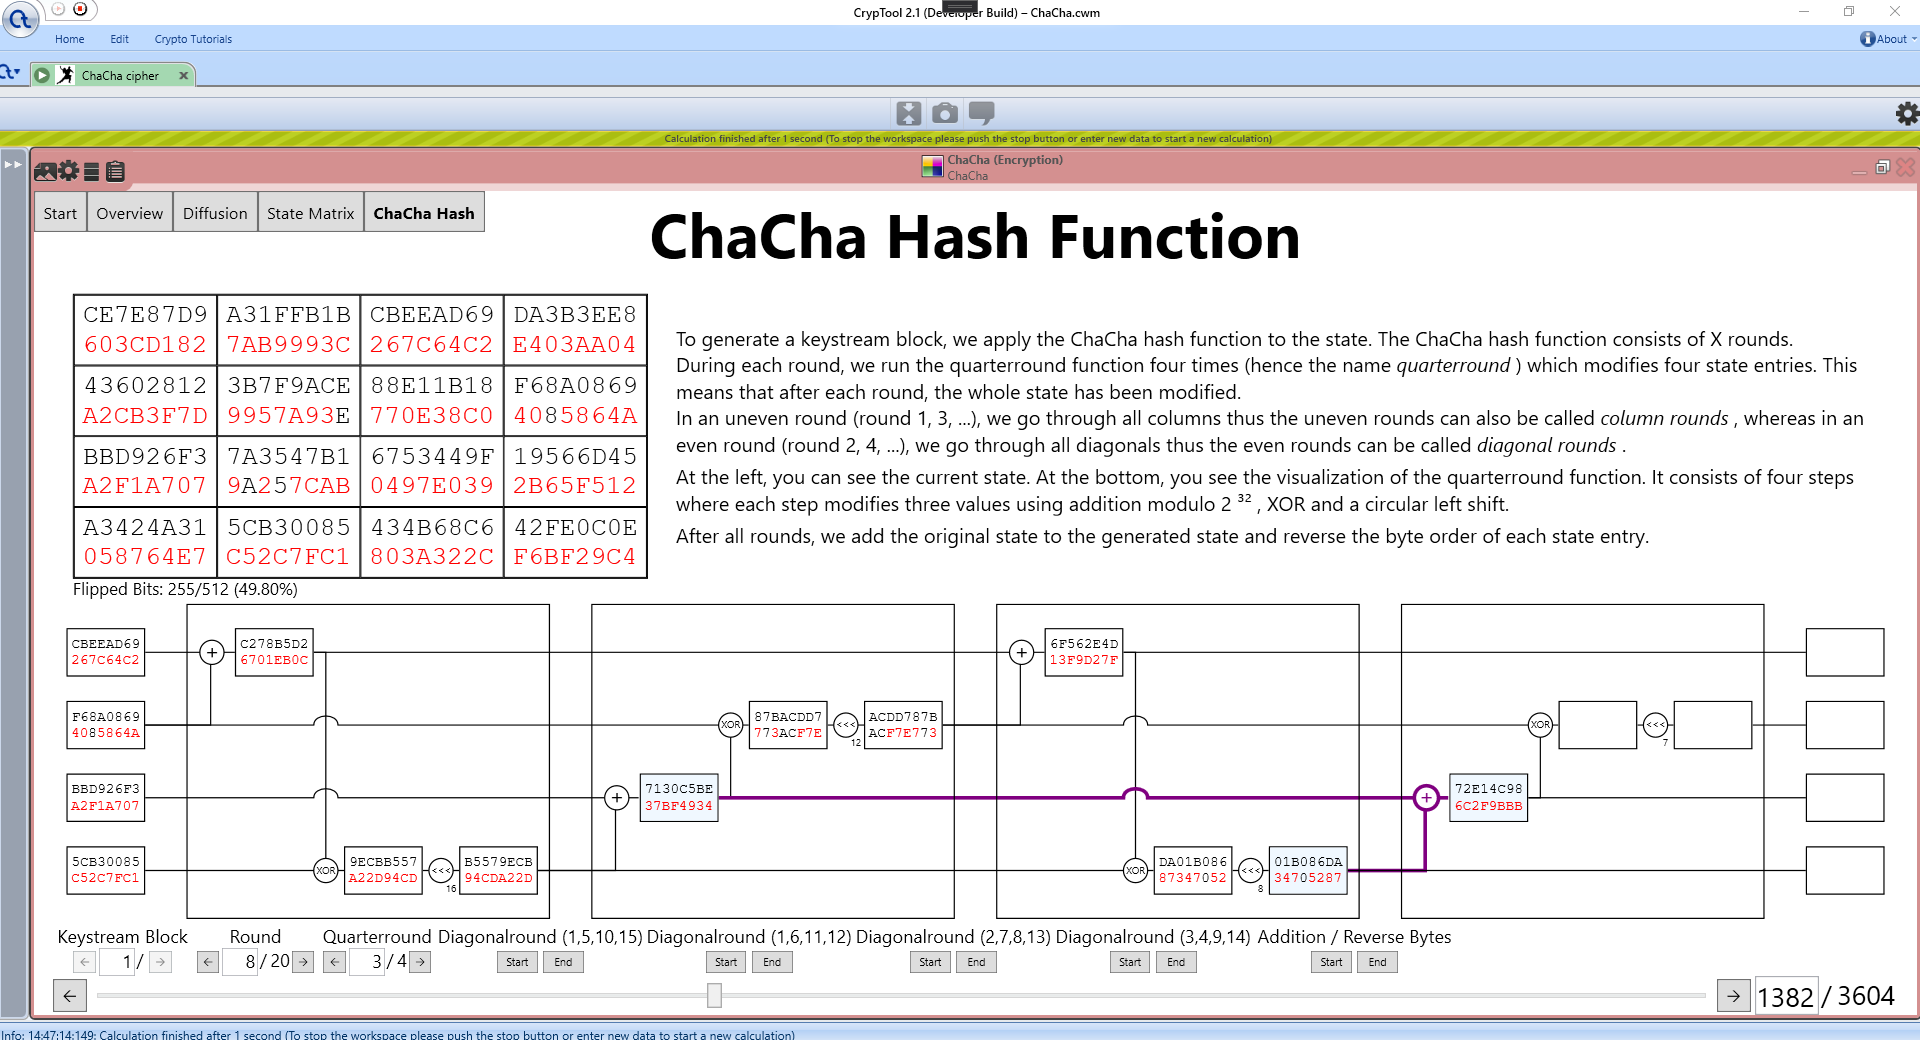
\includegraphics[width=\textwidth]{figures/ct2/chachahash/chachahash-mid-qr-diffusion.png}
  \caption{Quarter-round visualization with diffusion (showing both values)}
  \label{fig:chachahash.mid.qr.diffusion.both}
\end{subfigure}
\begin{subfigure}[t]{\textwidth}
  \centering
  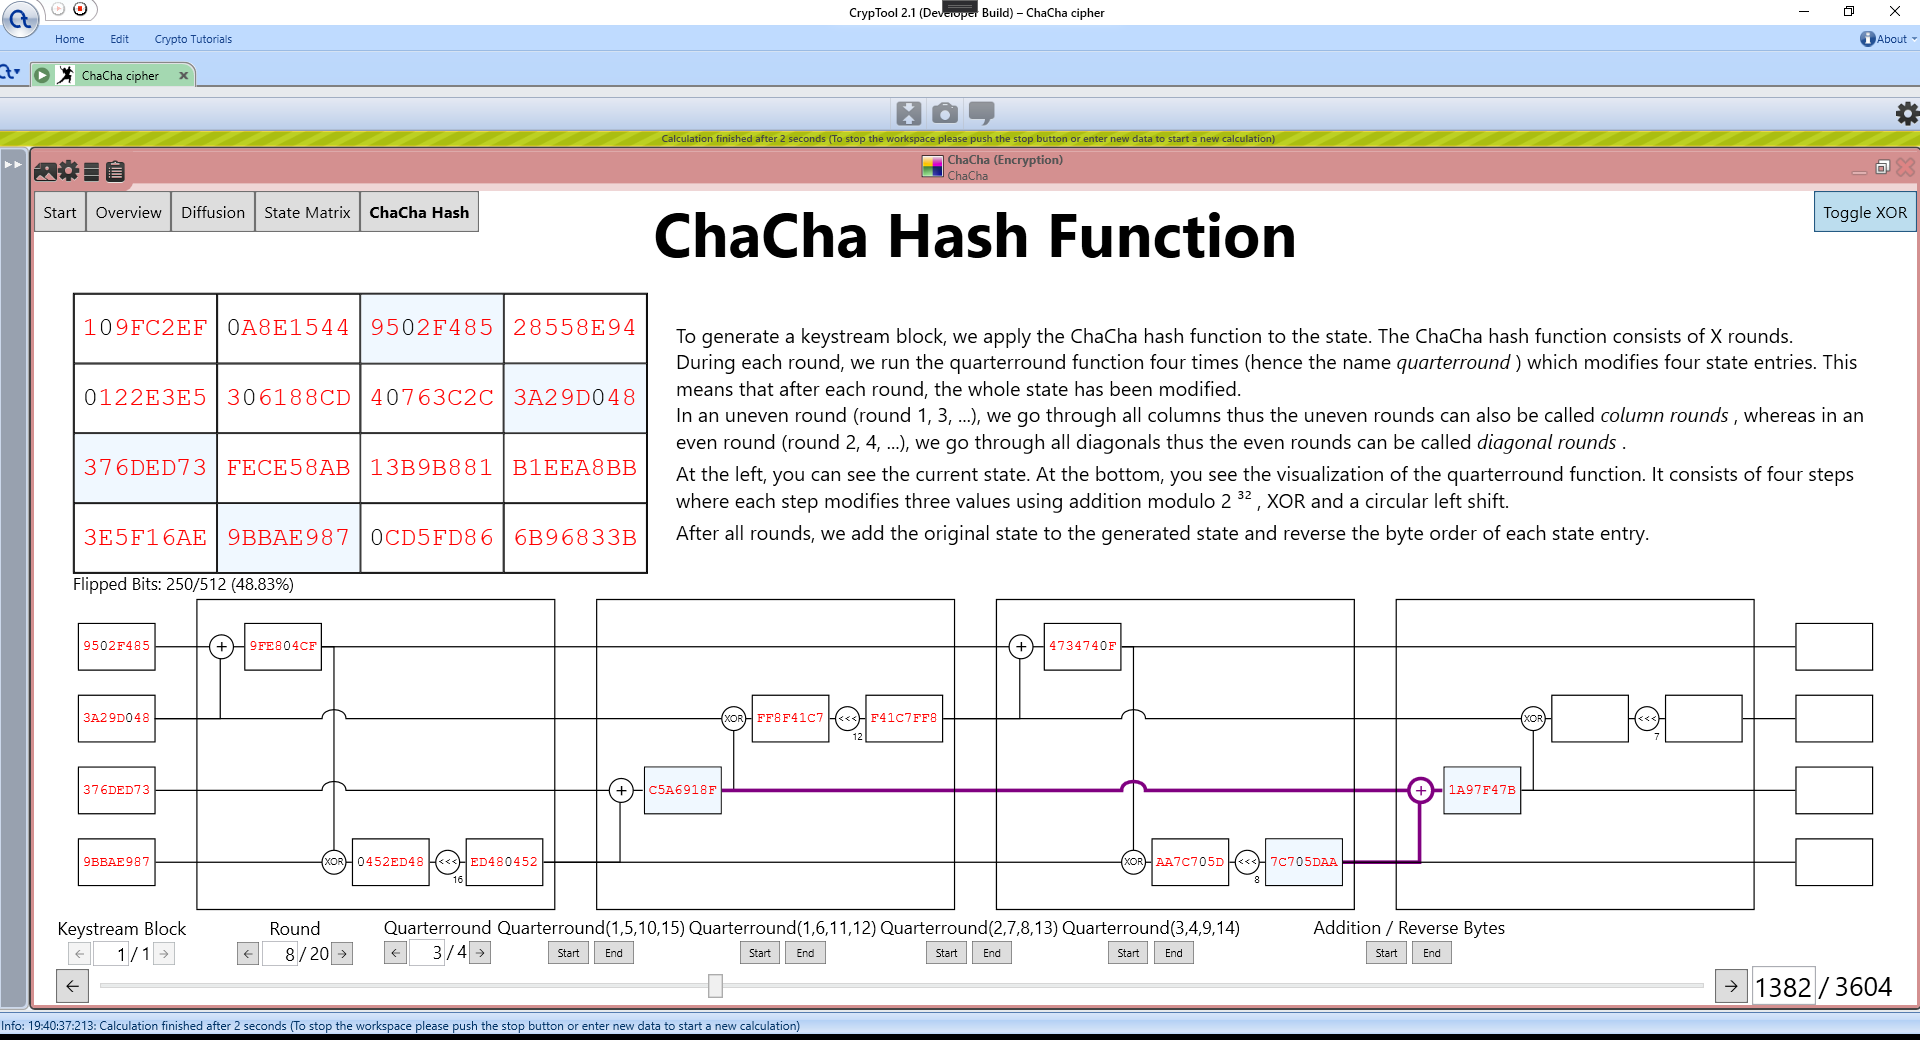
\includegraphics[width=\textwidth]{figures/ct2/chachahash/chachahash-mid-qr-diffusion-xor.png}
  \caption{Quarter-round visualization with diffusion (XOR)}
  \label{fig:chachahash.mid.qr.diffusion.xor}
\end{subfigure}
\caption{Quarter-round visualization with diffusion}
\label{fig:chachahash.mid.qr.diffusion}
\end{figure}


%%%%%%%%%%%%%%%%%%%%%%%%%%%%%%%%%%%%%%%%%%%%%%%%%%%%%%%%%%%%%%%%%%%%%%%%

\FloatBarrier
\subsection{Architecture}
\label{sec:Architecture}

In this section I will go more into detail how the software was layed out.

The software architecture, which was written using WPF (Windows Presentation Foundation), XAML and C\#7.0, can be split into two parts.

The first part is about the MVVM (Model-View-ViewModel) architecture to create the user interface which was explained in the previous section, using WPF built-in tools such as data binding, templates, converters and validation rules.

The second part is about the action navigation system which plays a huge role regarding performance. It powers the slider and buttons in the bottom row of each page. The page navigation is handled by the first part because it is very simple and uses MVVM design patterns.

\subsubsection{MVVM architecture}

I have used a MVVM architecture because in previous attempts, I have discovered that the code becomes quite complicated over time if one is not following a design pattern with its standards and rules. This makes it harder to fix bugs or implement new features. \\
Even though I tried to follow some self-chosen guidelines like naming conventions and which code should go where, most of the time I went the path of least effort to have results as fast as possible which I could showcase to my supervisors and ask for feedback. The internal code structure was of no importance as long as the feature worked. Only when I realized that it got too cumbersome to maintain this workflow, I read about using design patterns in WPF applications and found out that MVVM is the most popular design pattern to use in conjunction with WPF \cite{mvvm-wpf}.

As the name suggest, MVVM is all about separating the code into three parts: Models, Views and View Models.

Models hold the raw application data. In our case, this would be the classes which hold the values generated by the ChaCha cipher. It should be completely unaware of any view or view Model.

Views define how the data should be presented. They consist mainly of XAML code with as little code-behind as possible. They do not maintain their own state but rather use data binding to synchronize themselves with the data inside view models. Therefore, views are aware of view models and in fact depend on them to show any relevant data.

View models connect the model data with the views. However, they do not directly manipulate the views but just define properties and methods which implement the logic for user interactions. The views then use data binding to be notified about any property changes or call methods if a button is clicked etc. This means that view models should not rely on any code inside a view. This essentially decouples the backend from the frontend.

\begin{figure}
\centering
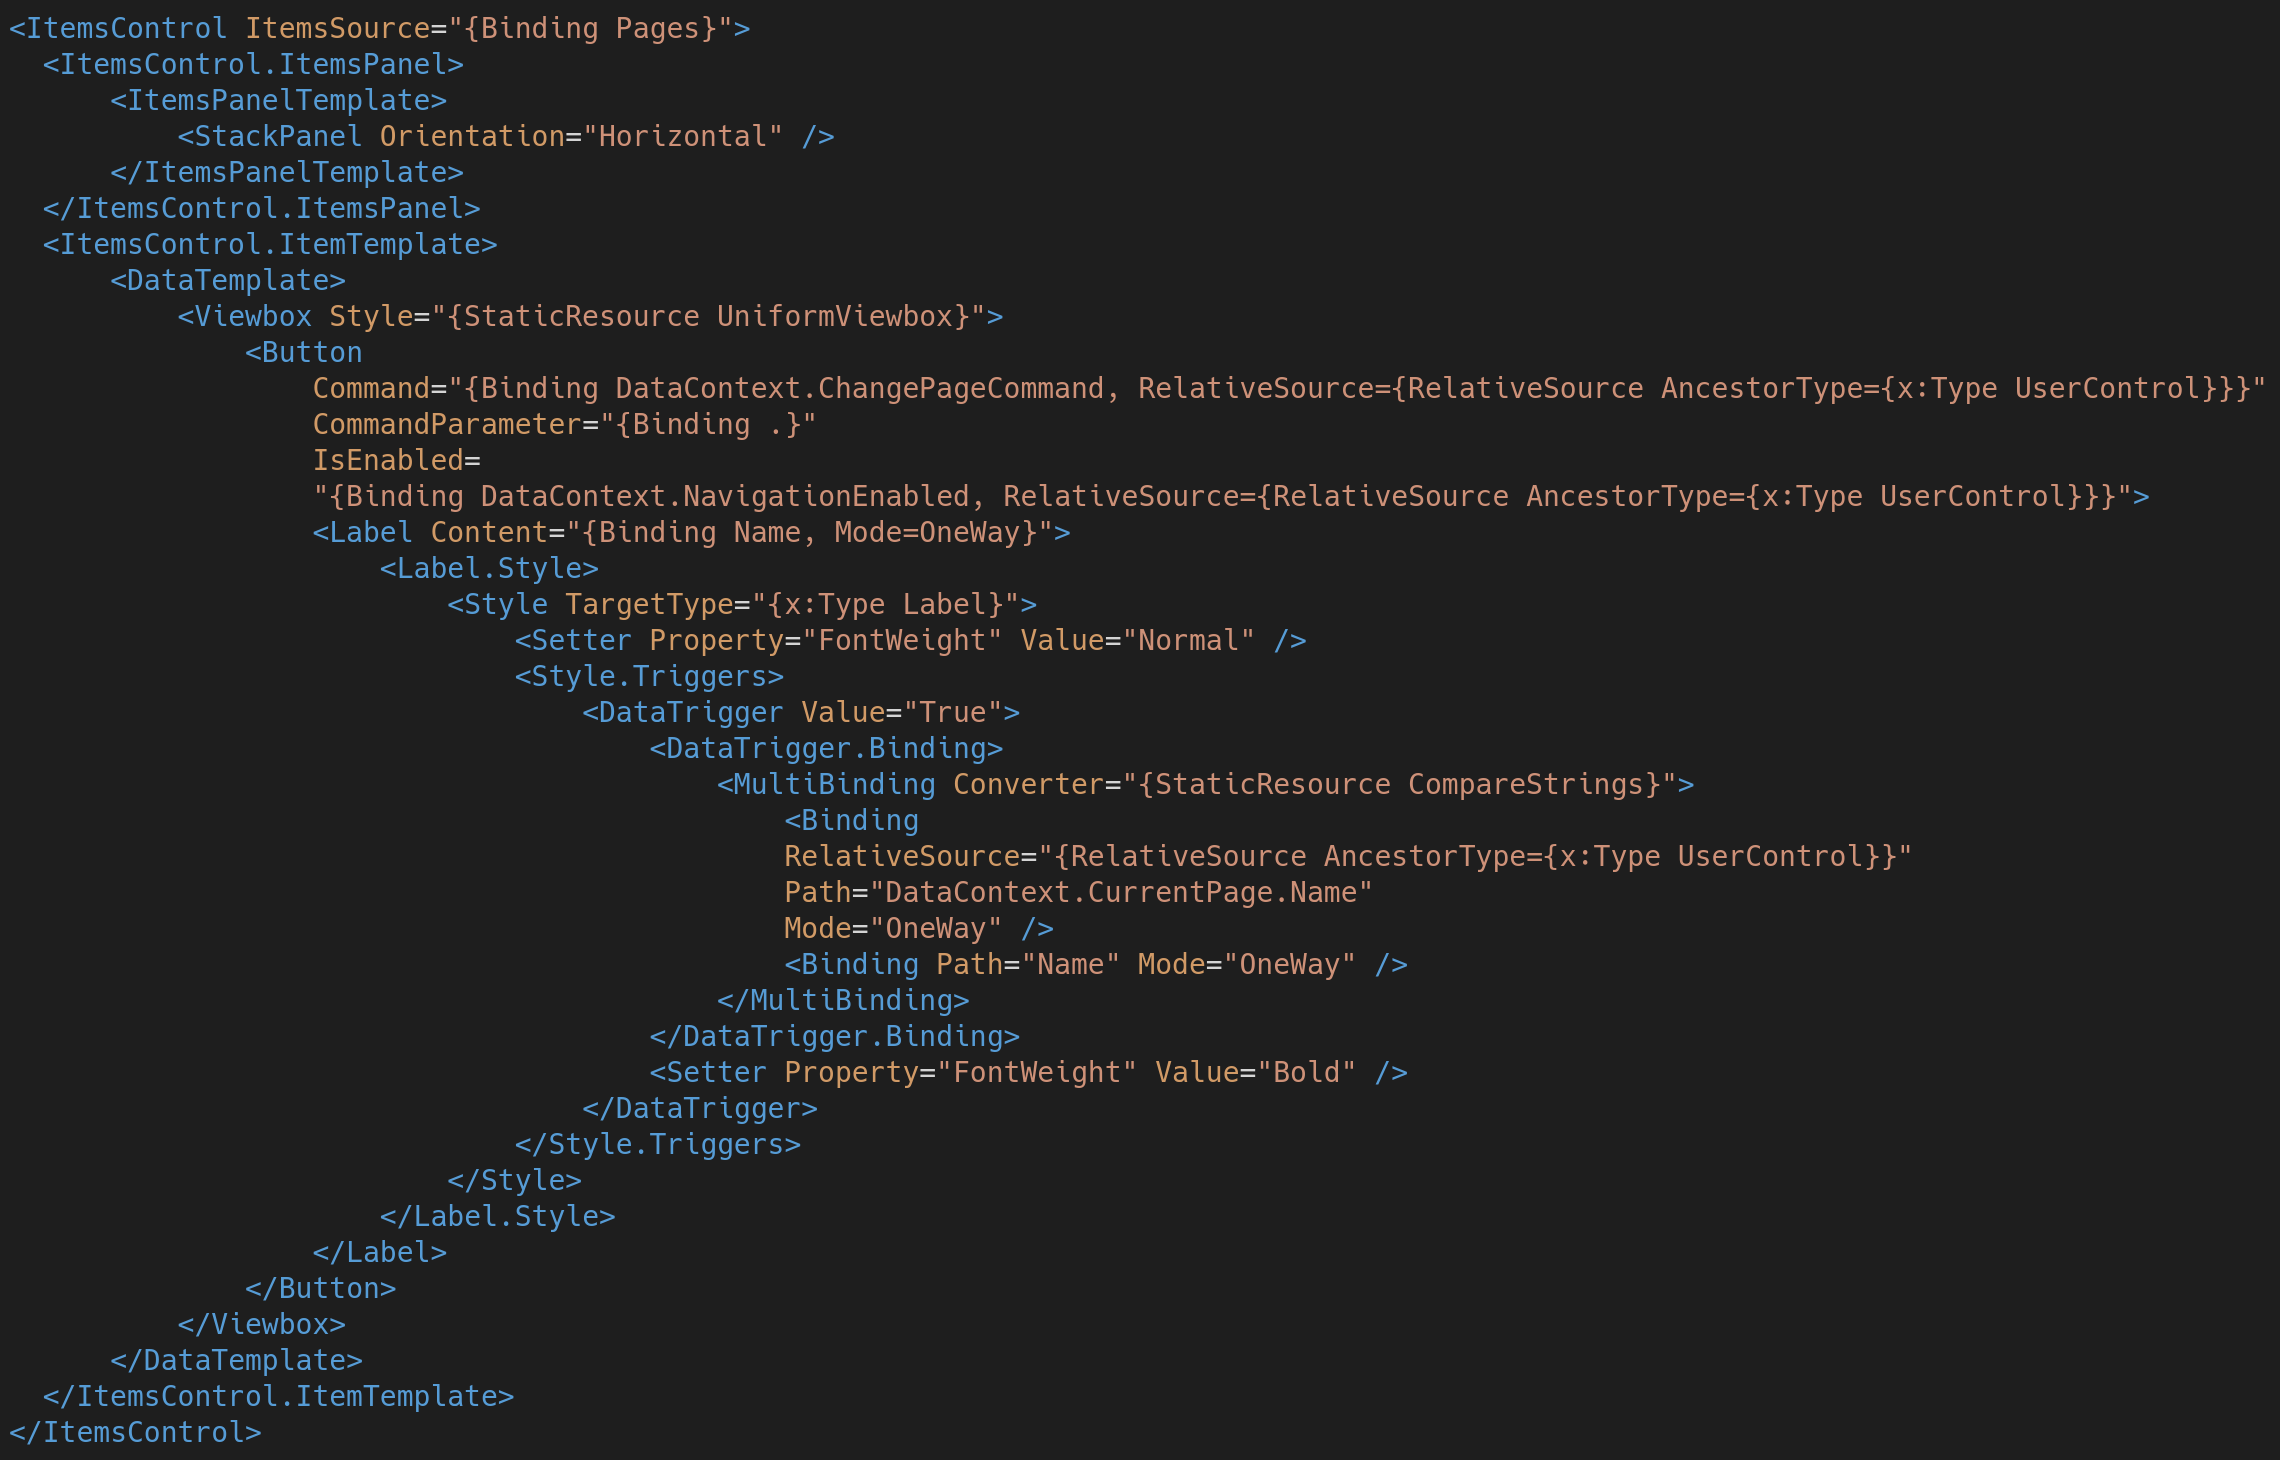
\includegraphics[width=\textwidth]{figures/code/mvvm-arch/page-navigation-template.png}
\caption[Page navigation]{Implementation of page navigation using data binding}
\label{fig:mvvm.pagenavigation}
\end{figure}

In Figure \ref{fig:mvvm.pagenavigation}, I have provided an example for how this data binding looks in code. What you see is the view code for the page navigation.

\begin{figure}
\centering
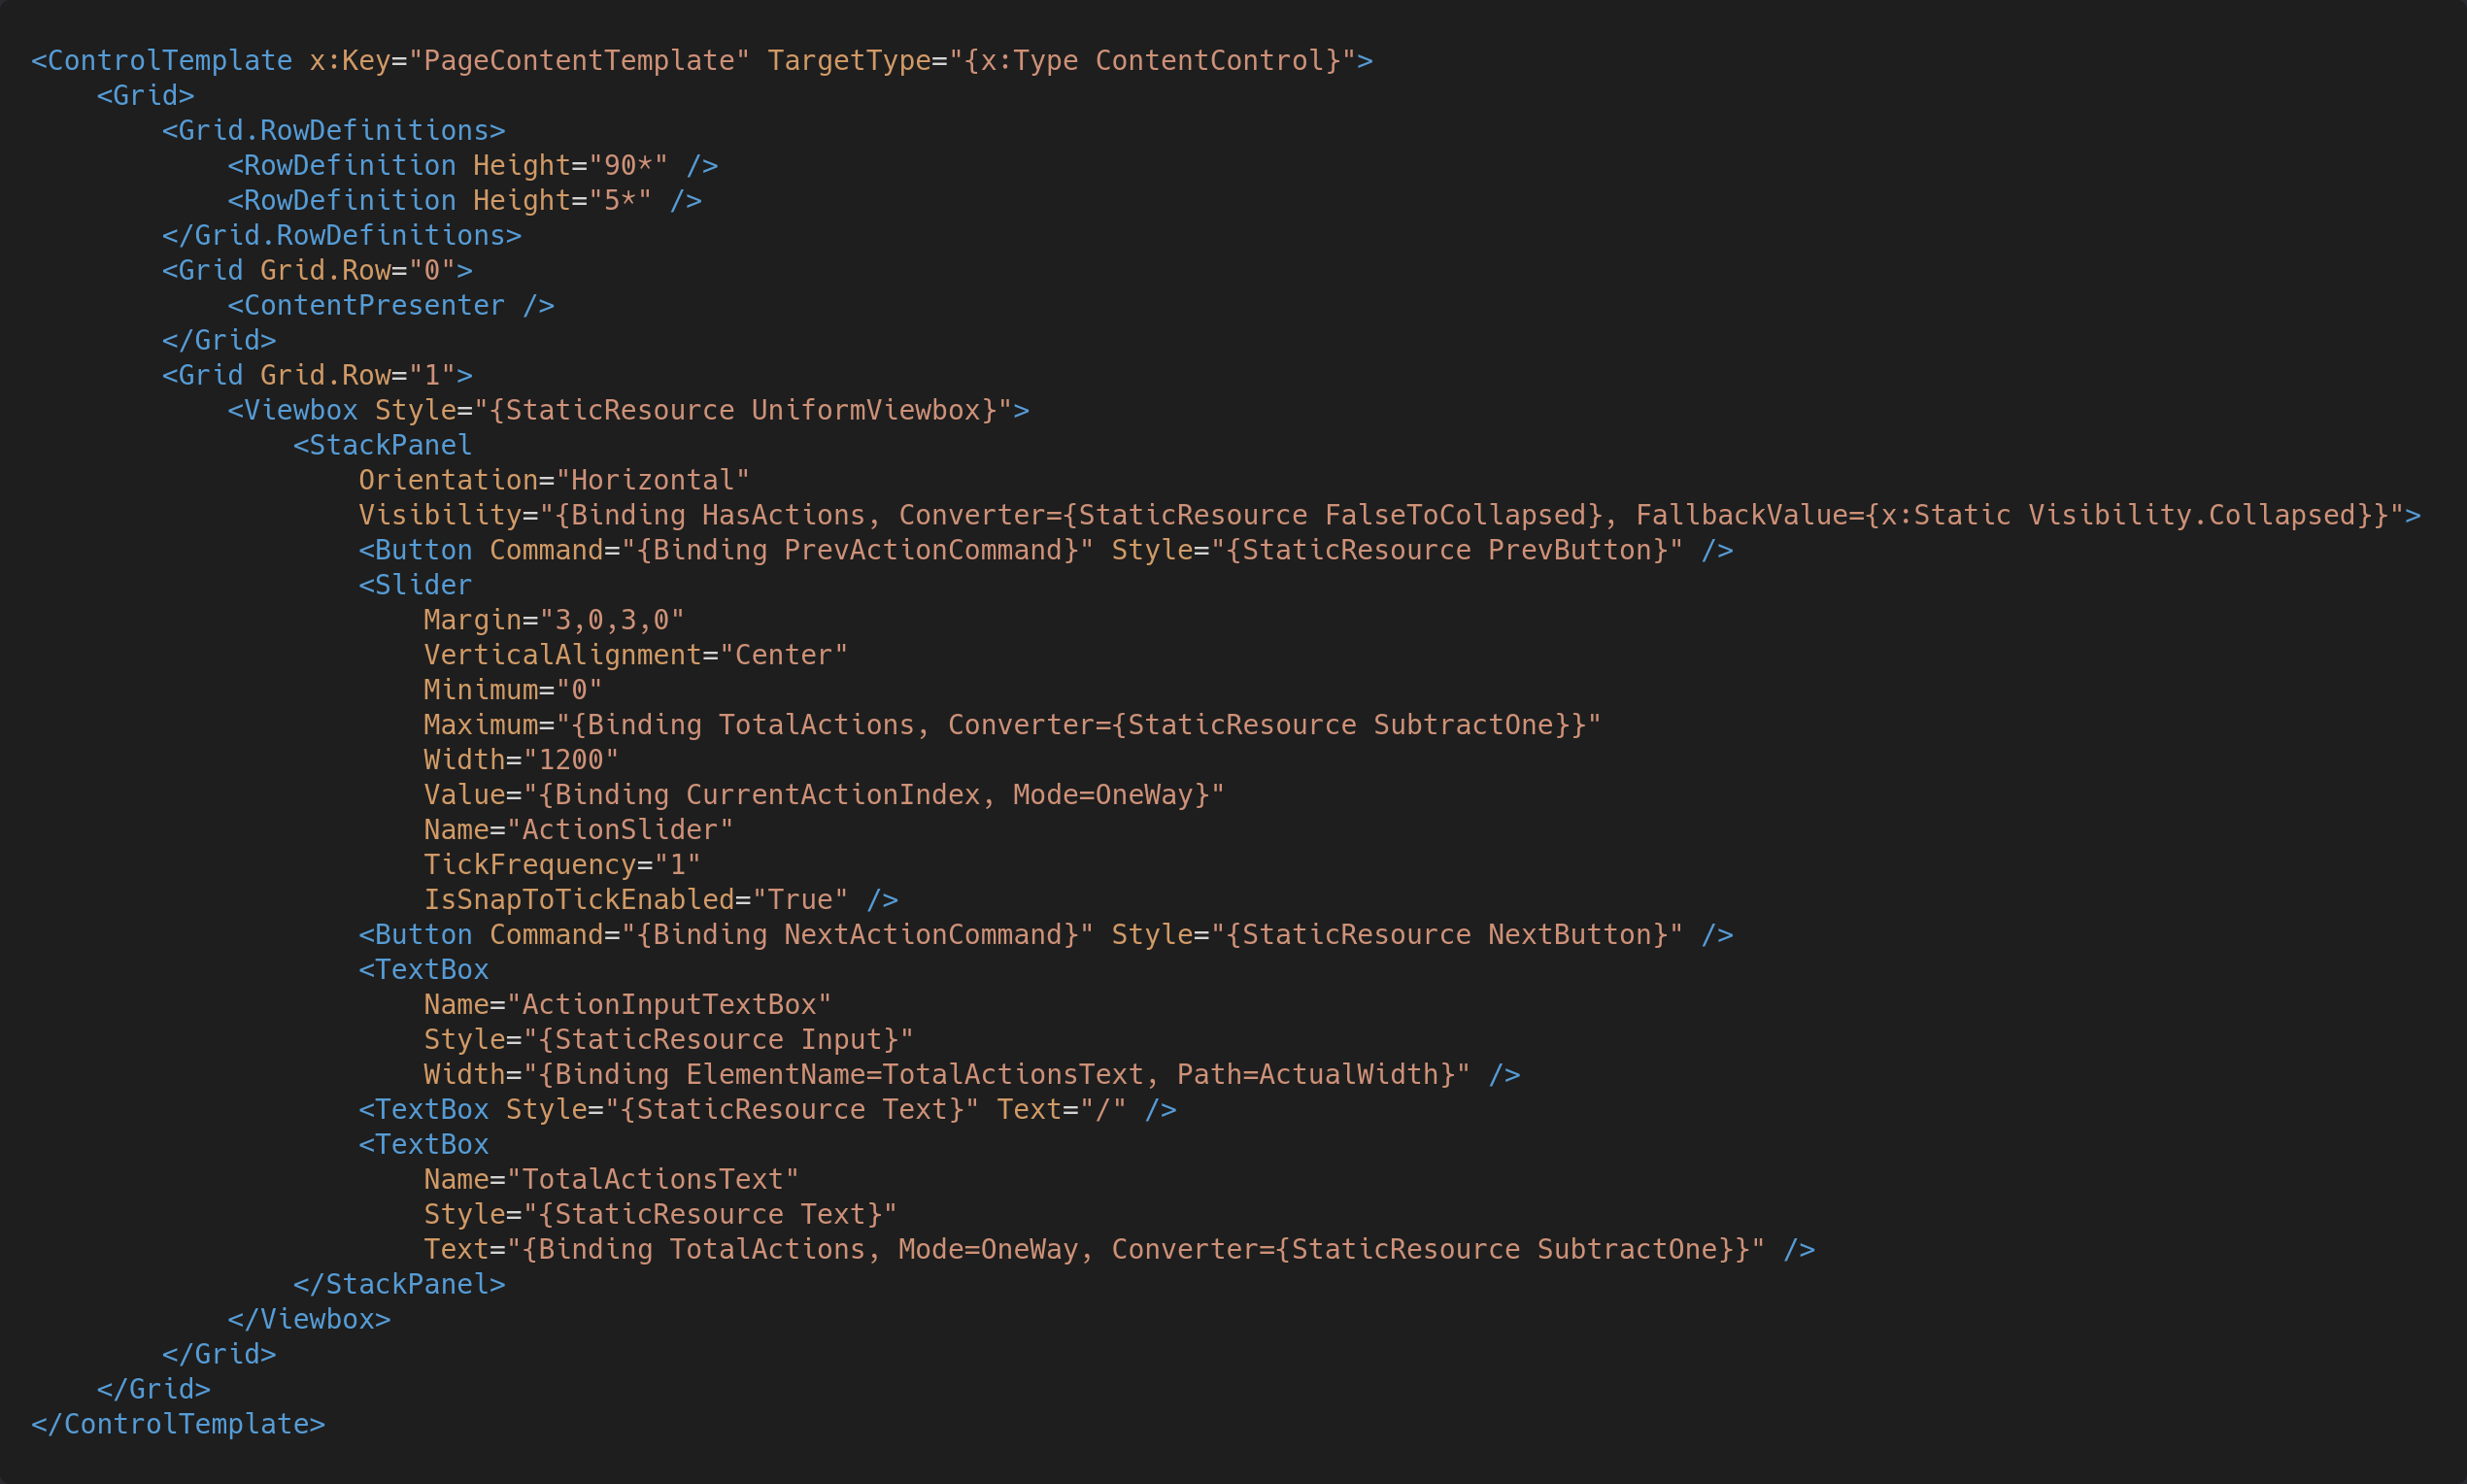
\includegraphics[width=\textwidth]{figures/code/mvvm-arch/action-navigation-template.png}
\caption[Action navigation]{Implementation of action navigation inside a control template}
\label{fig:mvvm.actionnavigation}
\end{figure}

Another technique (that you can also see in the mentioned Figure) is the use of templates. I have used data templates to attach views to view models and control templates to implement the general UI structure with the three sections I mentioned in Section \ref{sec:userInterface}. This enabled me to define the UI layout for all pages in one place and also reuse a single implementation of the page and action navigation across all pages. This way, view modifications down the road which applied to all pages were easy and fast. In Figure \ref{fig:mvvm.actionnavigation}, you can see the view implementation of the action navigation bar which is only visible on pages which do have actions.

Since the most interesting part about the MVVM architecture is probably how the diffusion visualization works, I will explain this feature in more detail.

\subsubsection{Diffusion implementation using MVVM}

If the user enters something into the input fields of the Diffusion page, validation of the input occurs. It checks if the input contains only valid hexadecimal characters and if the size is not too large. This is done by using two-way bindings and extending the \texttt{ValidationRule} class which is a built-in module of WPF. Only if the input is valid, the value is saved into a property of the underlying view model. This way, we can be sure that we always have sane data with which we later can execute the cipher with.

Furthermore, I am using converters which are also built into WPF to convert data into user-friendly formats. Converters are always attached to bindings, so inside the two-way bindings, I am converting the byte arrays into hex strings and vice versa.

Since data binding works by notifying the view if a variable has changed, WPF provides an interface named \texttt{INotifyPropertyChanged} which helps with implementing these data binding notifications. It provides a method named \texttt{OnPropertyChanged} and  an event named \texttt{PropertyChangedEventHandler} which must be called with the name of the variable to raise such an notification. The data binding system then updates the variables in the view.

\begin{figure}[!hbt]
\centering
\begin{subfigure}[t]{0.6\textwidth}
\centering
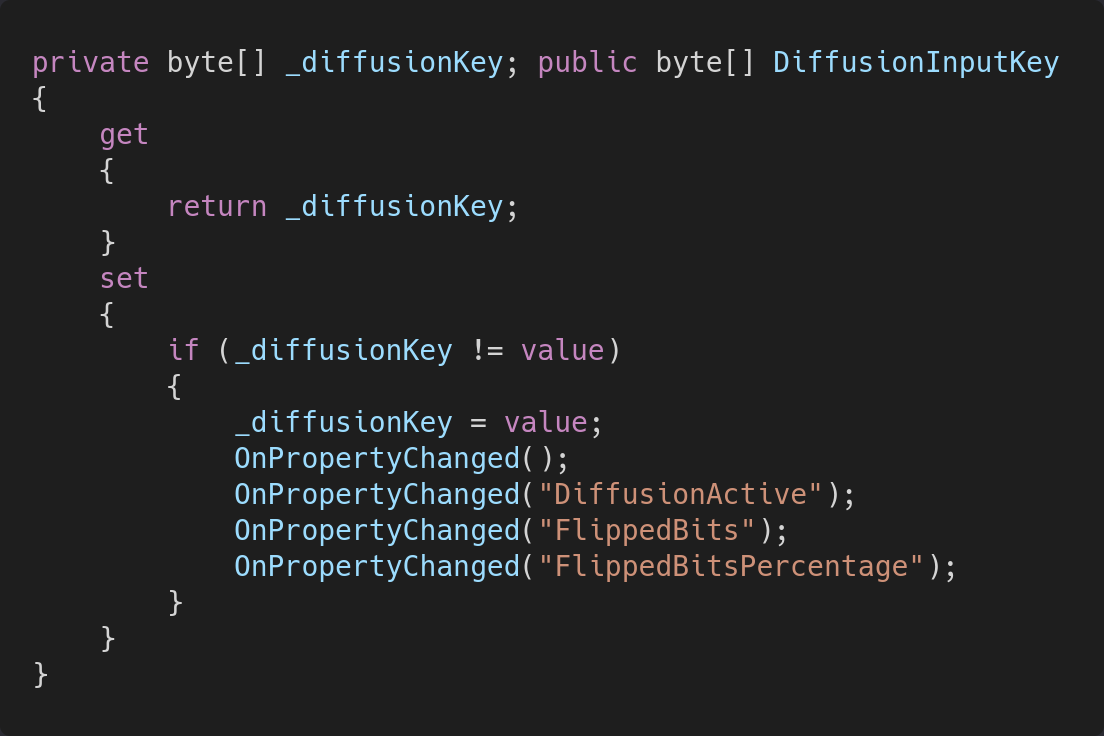
\includegraphics[width=\textwidth]{figures/code/mvvm-arch/onpropertychanged.png}
\caption{Data binding notification in setter of \texttt{DiffusionInputKey}}
\label{fig:mvvm.onpropertychanged}
\end{subfigure}
\begin{subfigure}[t]{\textwidth}
\centering
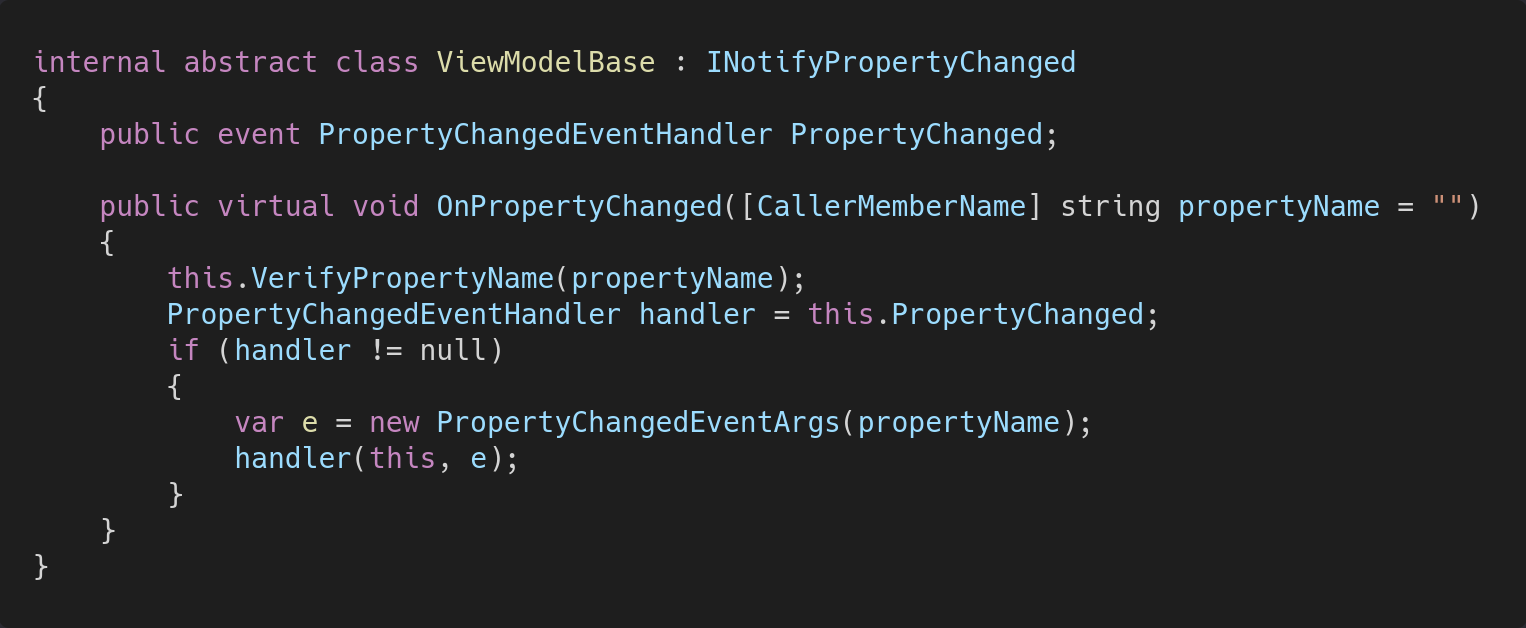
\includegraphics[width=\textwidth]{figures/code/mvvm-arch/viewmodelbase.png}
\caption{\texttt{ViewModelBase} implementation with \texttt{INotifyPropertyChanged} interface}
\label{fig:mvvm.viewmodelbase}
\end{subfigure}
\caption{Data binding notification implementation}
\label{fig:mvvm.databindingnotification}
\end{figure}

The notification raising and the implementation of the \texttt{INotifyPropertyChanged} interface can be seen in Figure \ref{fig:mvvm.databindingnotification}. The setter of \texttt{DiffusionInputKey} raises multiple notifications because other variables which depend on \texttt{DiffusionInputKey} also need updating. (The first call of \texttt{OnPropertyChanged}  in the setter has no argument because the attribute \texttt{CallerMemberName} in the function signature automatically enters the name of the caller if no argument is provided.)

On page exit, \texttt{ChaChaPresentationViewModel}, which is the view model which implements navigation between the different pages (which have their own view models), calls \texttt{Teardown} on the page we are leaving. This triggers the ChaCha execution with the given altered values.

Before execution, a flag was set which instructs the list getters into which the ChaCha component would save its intermediate values to return a different list. This means that the ChaCha component is agnostic of where it ultimately saves its intermediate values. During the execution, the intermediate values for the diffusion run are therefore saved in parallel lists. This is shown exemplary for the quarter-round input values in Figure \ref{fig:mvvm.chacha}. The other pages then simply bind to these lists to display the intermediate values of the diffusion run. Converting the 32-bit unsigned integers into hex strings and marking their characters which are different red is then done in the view models.

\begin{figure}
\centering
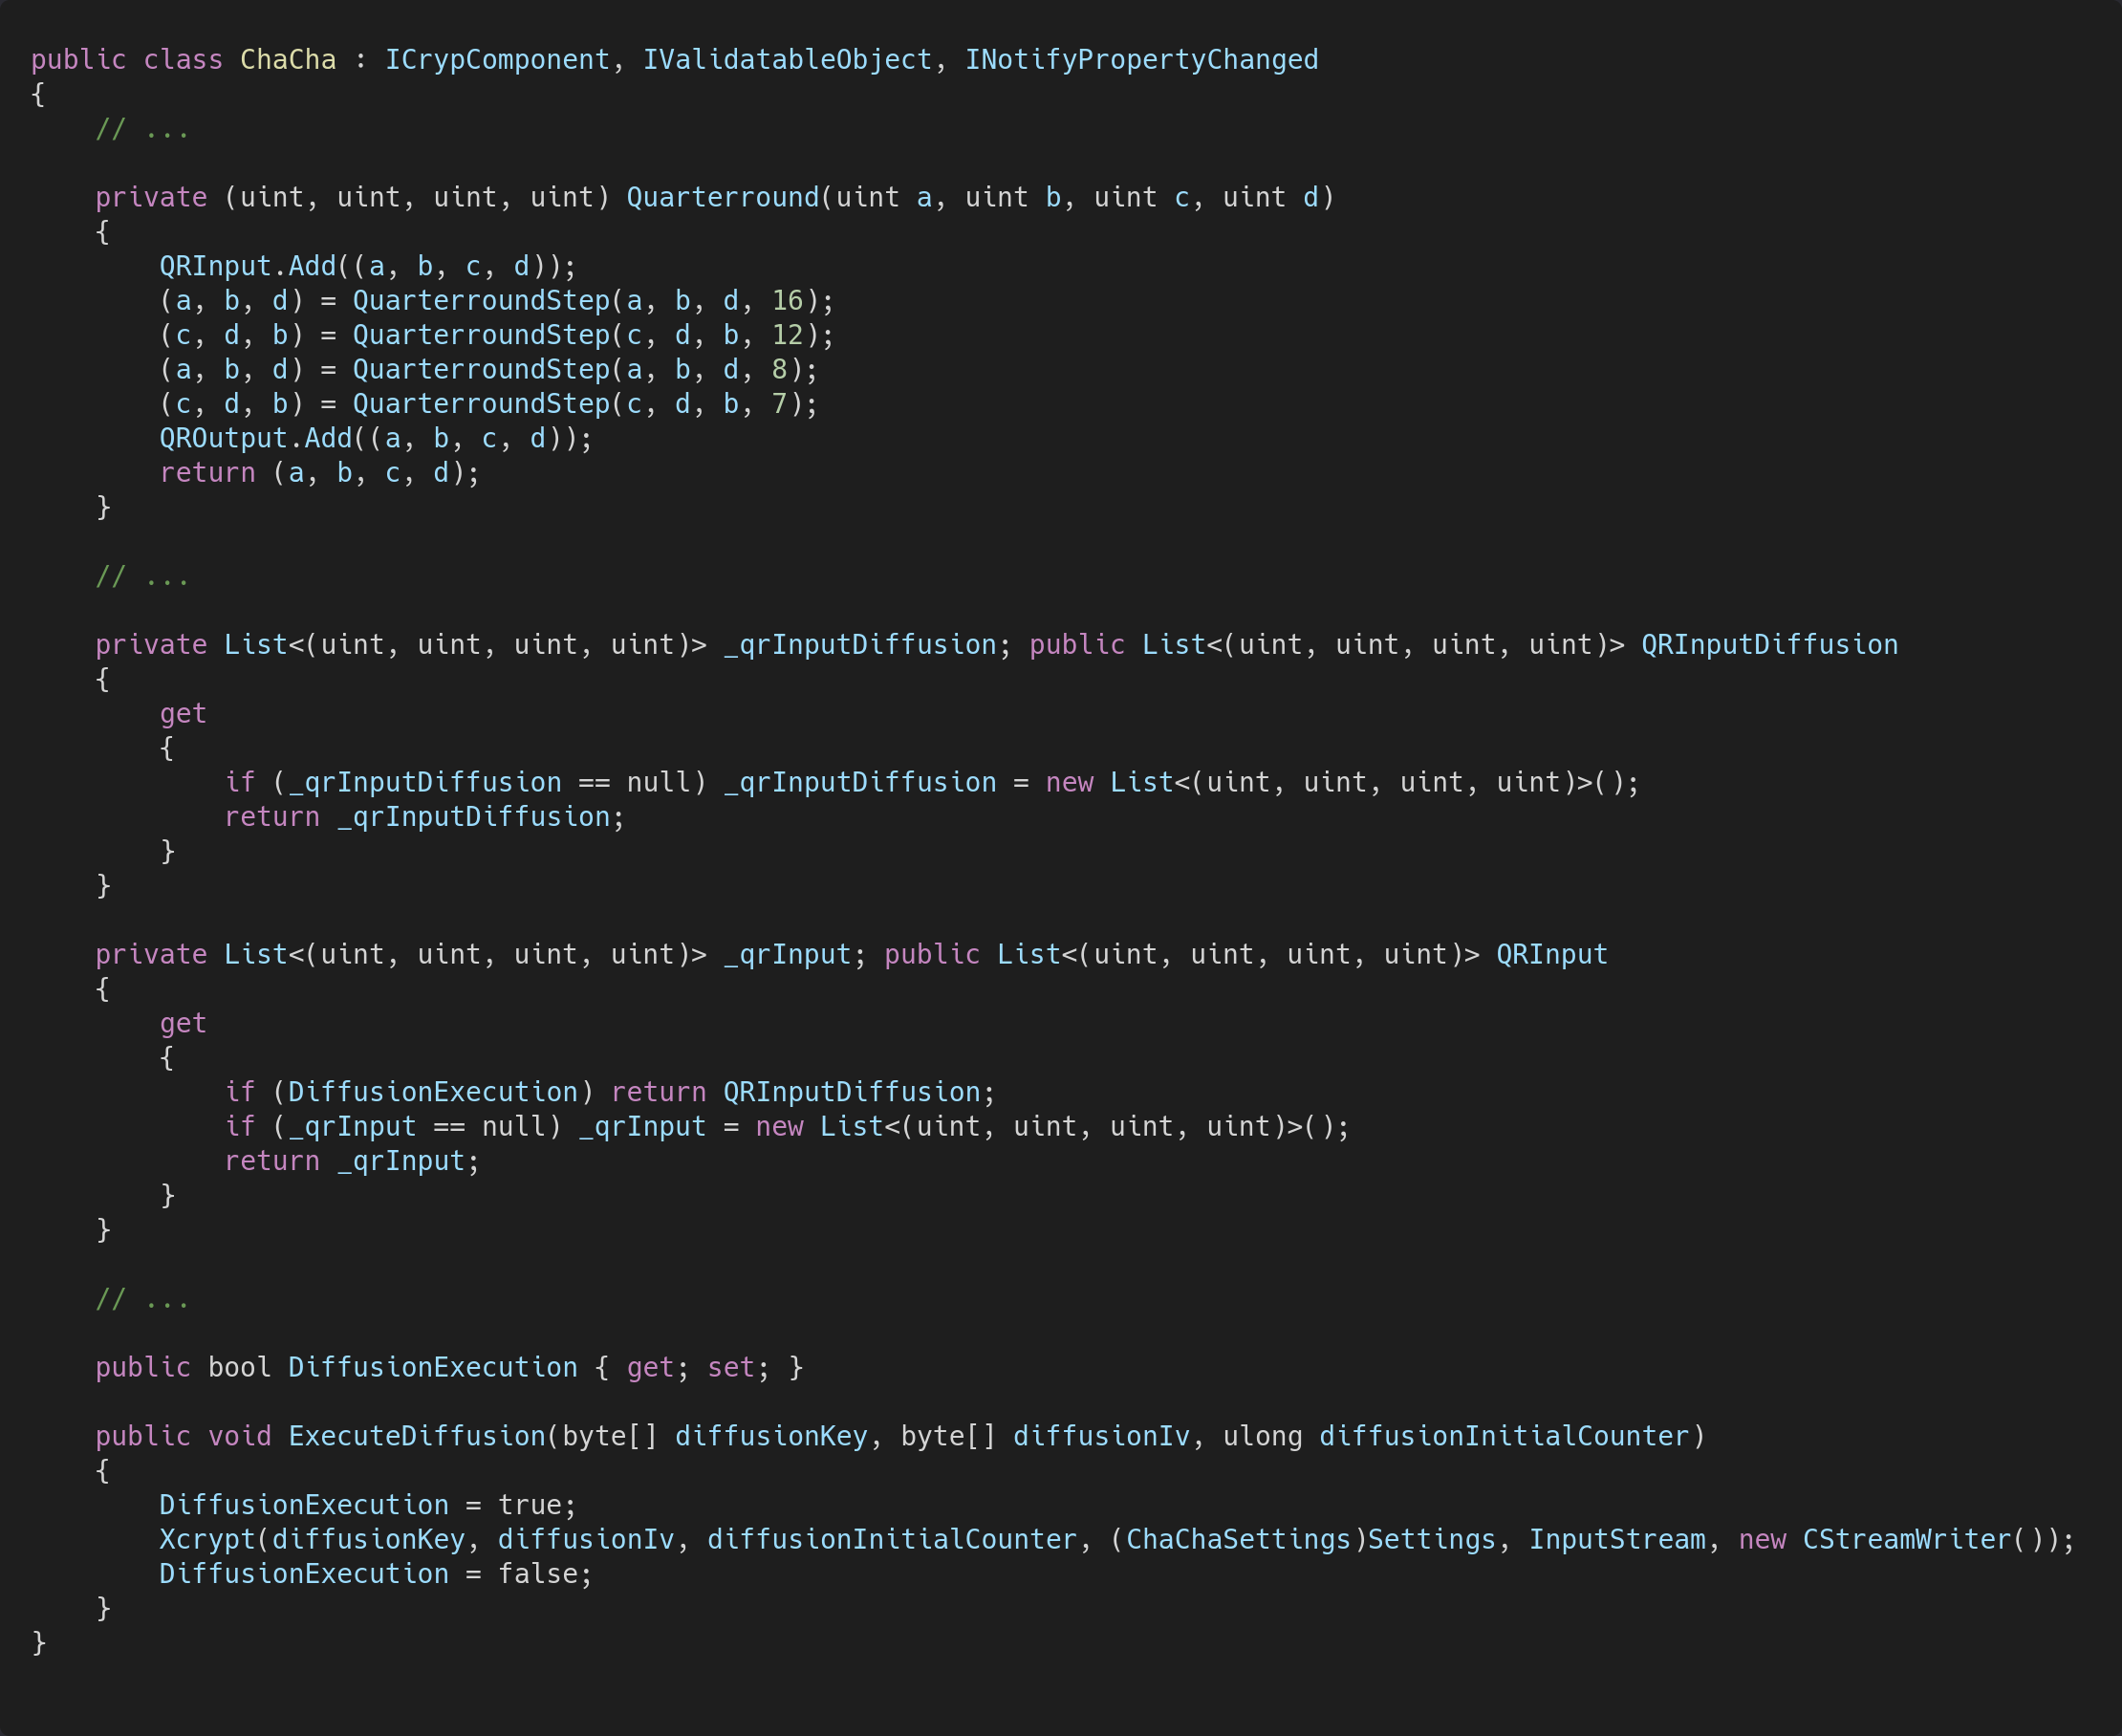
\includegraphics[width=\textwidth]{figures/code/mvvm-arch/chacha.png}
\caption[Intermediate values saving]{Saving of intermediate values during ChaCha execution in lists}
\label{fig:mvvm.chacha}
\end{figure}

\vfill

\FloatBarrier

\subsubsection{Centralized navigation system}

\begin{figure}
\centering
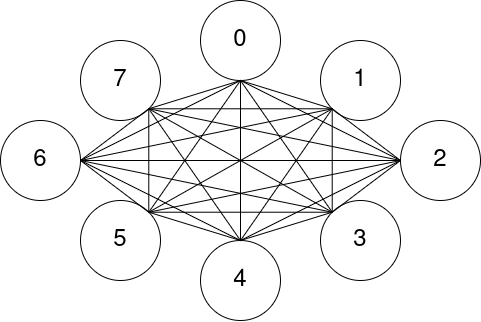
\includegraphics[width=0.5\textwidth]{figures/navigationsystem-diagram/navigationsystem-all-overview.png}
\caption[Navigation paths (no reset state)]{Navigation paths between actions if no reset state was used.}
\label{fig:navsystem.all.overview}
\end{figure}

The final design of the navigation system was characterized by reflecting on the problems previous iterations had. In this subsection, I will only describe the current, final implementation of the navigation system. The previous implementations with their problems are described in Section \ref{sec:encounteredProblems}.

The core idea of the navigation system was to decrease hops between actions without having too many possible transitions since for every transition from action $A$ to another action $B$ and vice versa, code needs to be written to perform the transition. Figure \ref{fig:navsystem.all.overview} shows how a navigation system would look like where the maximum amount of hops is minimized to one. Total transitions are $2n(n-1)$ and for every new action, transitions increase by $2(n-1)$ ($n$ is the total number of actions). The factor 2 comes from the fact that for every transition from action $A$ to $B$, we also need a transition back from $B$ to $A$. We can conclude that such an architecture does not scale very well from the perspective of a developer who needs to write all of that transitional code. \\
On the other hand, decreasing the amount of possible transitions by introducing more hops would degrade performance due to computational overhead, so a system with a very high average amount of hops would not scale very well regarding performance.

\begin{figure}
\centering
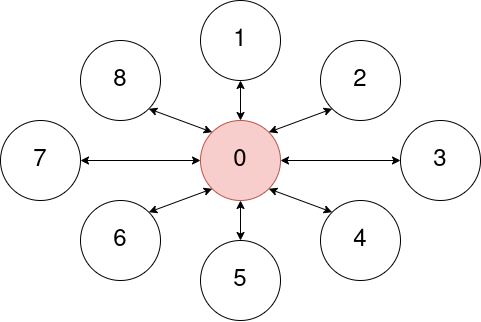
\includegraphics[width=0.5\textwidth]{figures/navigationsystem-diagram/navigationsystem-central-overview.png}
\caption[Navigation paths in centralized navigation system]{Navigation paths between actions in the centralized navigation system. \\The colourized state is the reset state which corresponds to the initial state.}
\label{fig:navsystem.central.overview}
\end{figure}

I came to the conclusion that the best trade-off would be to have a navigation system where every action has a transition to a centralized state and this central state then has a transition to all other actions. This would result in a maximum of two hops between any two actions. Further, adding a new action would only add two new transitions to the system. This system design is shown in Figure \ref{fig:navsystem.central.overview}.

During implementation, I realized I could bring the amount of new transitions for each action down to one. Defining the initial state as the central state meant that transitioning from any action to it could be done by just resetting the whole page to the first action. Due to this, I started calling the central state the reset or initial state since they were the same.

Unfortunately, I saw the issue of code duplication quickly arising with this design. Since most of the time, the next page state is only a slight modification of the previous page state, the code for following actions was almost the same. To mitigate this issue, I started to think about my actions as sequences. A sequence of actions would mean that every action inside a sequence is an extension of all previous actions of the same sequence. Extension in this context means that if action $A$ extends action $B$, action $A$ contains at least all the code of action $B$. To use terminology of set theory, one could also say that $A$ is a superset of $B$; viewing individual code statements as objects.

\begin{figure}
\centering
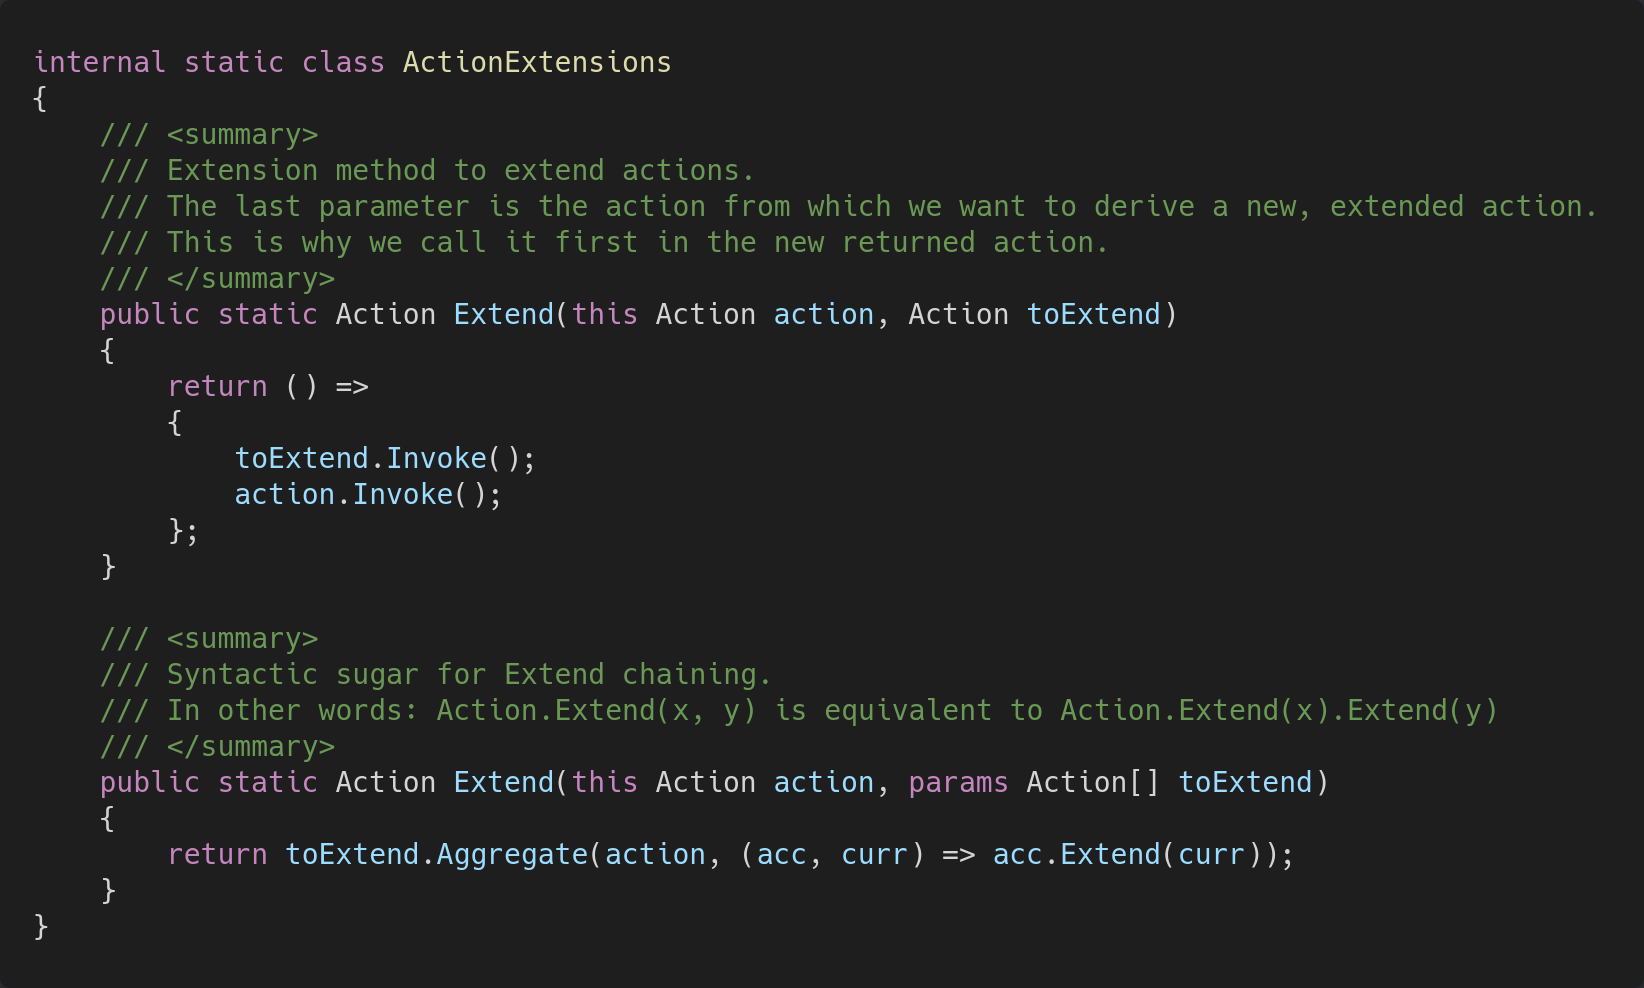
\includegraphics[width=\textwidth]{figures/code/nav-arch/action-extensions.png}
\caption[Extending \texttt{Action} type]{Extension method for the \texttt{Action} type to extend actions}
\label{fig:navsystem.sequences.extension}
\end{figure}

To implement this concept, I created an extension method for the \texttt{Action} type in C\# together with an interface to create action sequences. Figure \ref{fig:navsystem.sequences.extension} shows the method which extends the built-in \texttt{Action} type.

I also wanted nested sequences. This means that a sequence could be started inside another sequence. A nested or child sequence would extend all the actions from its parent sequence. From the perspective of the nested sequence, it is no different than if all the actions from the parent sequence were created inside it. When ending a nested sequence, from the perspective of the parent sequence, the nested sequence never existed. Figure \ref{fig:navsystem.test} shows a test which asserts that this nesting does indeed work as expected.
\begin{figure}
\centering
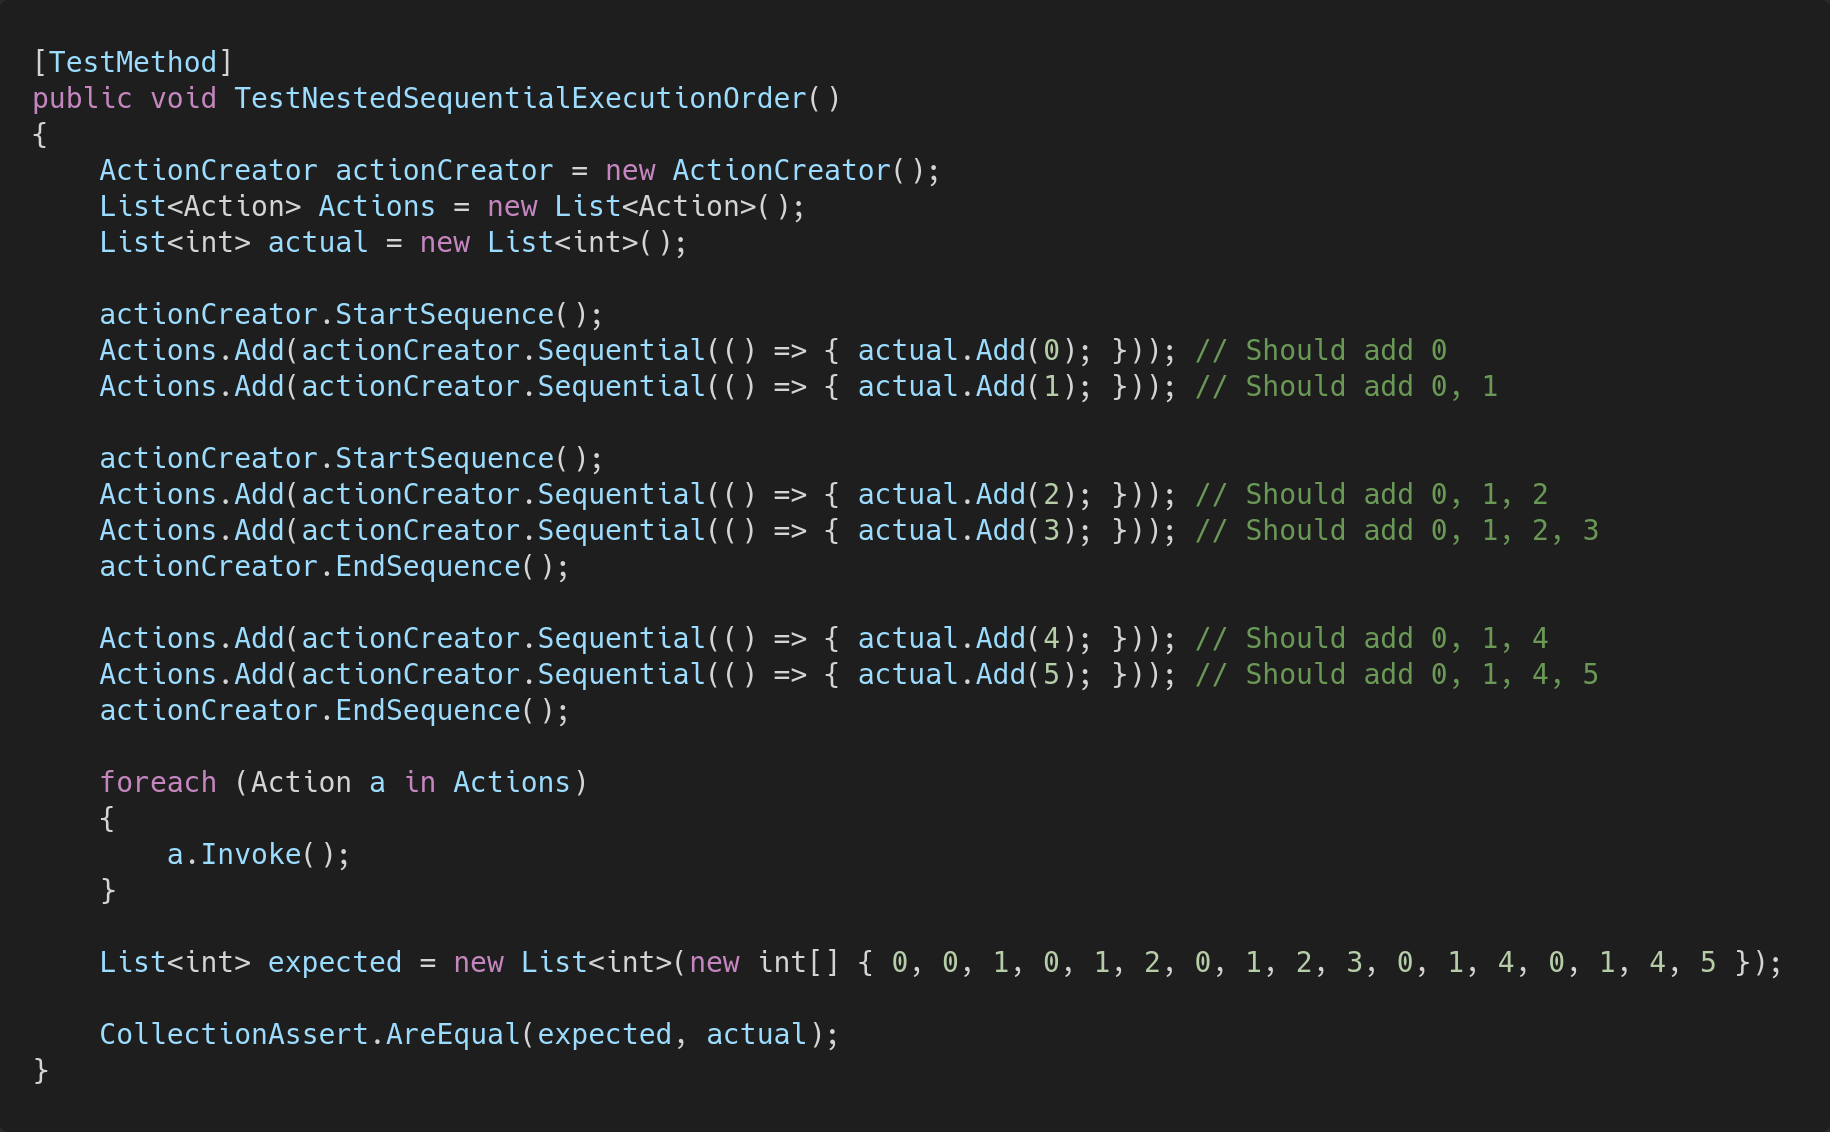
\includegraphics[width=\textwidth]{figures/code/nav-arch/TestNestedSequentialExecutionOrder.png}
\caption{Test method for nested sequences}
\label{fig:navsystem.test}
\end{figure}

This was very helpful for implementing the actions for the ChaCha Hash Function page. Since each keystream block started with a cleared quarter-round visualization and the initial state visible in the state matrix, it made sense to declare a sequence for each keystream block. The same was true for each round and quarter-round. This meant that I would not introduce too much computational overhead inside the transitional code (even though only one transition was executed by design) since I could just reset the sequence if it made no longer sense to include the code of previous actions.

Essentially, this prevented the system degrading back to a linear navigation system as will be described in Section \ref{sec:encounteredProblems}. The system would have less transitions but would still execute the same code as a linear navigation system would when moving from action 0 to any other action; undoing any positive effect this approach of minimizing transitions could have had.

The weakness of this design was that there was still some overhead when navigating through the page in a linear manner since the system is basically designed to always go back to the first action first and from there to the desired action. This leads to a lot of unnecessary resetting because as mentioned, most of the times the next page state is only a slight modification of the previous one. But this is the trade-off I had to make for a good overall performance. To summarize, this design had a higher overhead for small steps but did scale much better for bigger steps which were necessary for the keystream, round and quarter-round navigation.

%%%%%%%%%%%%%%%%%%%%%%%%%%%%%%%%%%%%%%%%%%%%%%%%%%%%%%%%%%%%%%%%%%%%%%%%

\section{Encountered Problems}
\label{sec:encounteredProblems}

In this section, I will discuss the main problems I encountered during implementation. To briefly summarize, they mainly consisted of how the system behind the interface should be designed to have the best or at least a reasonable performance.

The author of the AES visualization has mentioned in his thesis that to create a fluent user experience where he can navigate back and forth between all steps, the intermediate values need to be calculated beforehand and saved since we don't want to stop at each step to calculate the next value or recalculate everything from the start if the user wants to go backwards. I came to the same conclusion. But as I will describe on the next pages, this was not all that was needed to ensure such an experience.

I hope that the description of these problems and the solutions I have found may help future students in writing their own plug-ins.

\subsubsection{Linear navigation system}

\begin{figure}
\centering
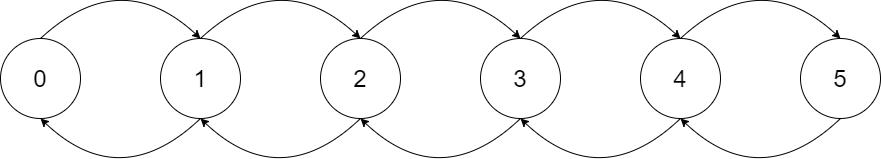
\includegraphics[width=\textwidth]{figures/navigationsystem-diagram/navigationsystem-linear-overview.png}
\caption[Navigation paths in linear navigation system]{Navigation paths between actions in the linear navigation system}
\label{fig:navsystem.linear.overview}
\end{figure}

The performance of the plug-in was essentially coupled to how the navigation system was designed. Other things like the aforementioned calculation of the intermediate values for the visualization were compared to the navigation system design insignificant because they are created by the ChaCha cipher anyway and must just be saved somewhere to not lose them. This means that storing them was only a necessary but not sufficient condition for a overall good performance. \\
I realized this early in development when I had my first page with many page actions on it and wanted to skip ahead a lot of actions. While implementing this feature which would enable the user to skip from any action to any other action, I realized that when skipping more than 100 actions, it already took about 750ms during which the UI was unresponsive. As can be seen in Figure \ref{fig:navsystem.performance.linear}, this time increased linearly so it was quite clear that I needed to do something about this, especially because the page with the most actions had over 3000 actions. All measurements were taken by starting at action 0 and skipping to the action specified at the x axis.

The root cause of the problem was the navigation system design which I called in hindsight \textbf{\textit{linear navigation system}}. It consisted of defining actions which build upon each other. This means that if we are at action 0 (initial state of the page) and want to go to action 5, we need to execute all the code inside the action definitions between 0 and 5 to arrive at the page state as it should be at action 5. This is resembled in Figure \ref{fig:navsystem.linear.overview}. \\
I came up with this design to have a smooth implementation experience where I only have to write the actual page state changes between two actions instead of duplicating a lot of code since the page state changes which were applied during a previous page were most of the times still visible when moving to the next action. This complements how the user experiences the visualization because the actions are numbered in a sequence and thus are inherently linear. Because of this, it made a lot of sense to me to reflect this in the system architecture.

Since this "design flaw" was not the leading cause of the performance problem (going through a for-loop of size 3000 does not directly lead to performance issues), I want to briefly explain how the actual action implementation looked like.\\
During the transition between two page states, the state of the page elements which will change is saved such that we can undo the changes if the user decides to navigate back. This enabled me to skip writing transitional code for backwards navigation, since I could just write a function which retrieves the state corresponding to the transition and then applies it. This function would then work for all backwards navigation without further intervention which was very convenient during development. \\
The problem with that architecture was that the state saving and the execution logic inside the action definitions were changing a lot of page elements directly by accessing them via their name that I gave them in the XAML code. That this was against best practices in writing WPF applications I only noticed later on, when I read more about them. This issue combined with the restricted, linear pathing between actions resulted in that huge performance loss that was described in Figure \ref{fig:navsystem.performance.linear}.

\subsubsection{Linear navigation system with caches}

After identifying the two underlying issues, I implemented what I called a \textbf{\textit{linear navigation system with caches}}. As the name suggests, I implemented cache entries to be able to navigate in constant time between an action and an action for which I created a cache. To not only increase performance during these transitions but between all transitions, we check before each transition, if first moving to a cached entry would decrease the amount of hops needed to go to our destination. \\
The cache entries consisted of instructions to restore the complete state of a page at the action index for which this cache entry was for. They contained instructions for the complete state instead of only the difference between two actions because now, moving to that cache must initialize the page, independent at which action / page state we were before. This means that there was some overhead in initializing the page because essentially, I cleared the whole page and then initialized the page elements with their appropriate content, potentially leading to some unnecessary code execution because the content prior to cleaning was already the one we needed. 

\begin{figure}
\centering
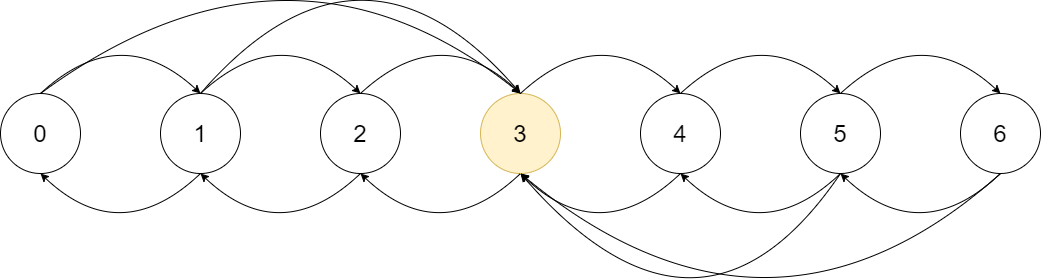
\includegraphics[width=\textwidth]{figures/navigationsystem-diagram/navigationsystem-cache-overview-2.png}
\caption[Navigation paths in linear navigation system with caches]{Navigation paths between actions in the linear navigation system with caches. The colourized state has a corresponding cache entry.}
\label{fig:navsystem.cache.overview}
\end{figure}

Figure \ref{fig:navsystem.cache.overview} demonstrates that the navigation system now needs less hops between any two given actions. Creating a cache entry for every start of a round increased performance significantly as can be seen in Figure \ref{fig:navsystem.performance.qr}. The maximum response time went down from 40 seconds in the system without any caches to 1.5 seconds. This could further be decreased to 200 milliseconds by creating cache entries for every start of a quarter-round (see Figure \ref{fig:navsystem.performance.qr}). Since it was not feasible to time every single data point, the data points marked as squares were just interpolated using previously timed data points. This means that for example, for the interpolated cache data points, I took the average of all previous measurements for skips to cached actions.

Further, to decrease the load on the CPU while dragging the action slider, I implemented a very simple asynchronous navigation. It was implemented by using a stack as a buffer for the values received from the slider during dragging. Every 50ms, the last value from the buffer is read and the page moves to that action. Afterwards, the buffer is cleared. \\
This did only enhance the slider but not the overall performance because at its core, it used the same navigation logic; just asynchronously. Nonetheless, it improved the performance during dragging significantly which I found quite impressing for how minimal the code for it is. In fact, the whole code for the asynchronous navigation can be seen in Figure \ref{fig:async.navigation}.

One of the major drawbacks for this enhanced design was that the automatic action undoing was no longer possible. Since we can not guarantee that the state between two actions has been saved, we cannot use our undo function. The reason is that any transition between two actions may have been skipped because first moving to a cached entry needed less hops. Therefore, I needed to write the code for backwards navigation to support caching.

\begin{figure}
\centering
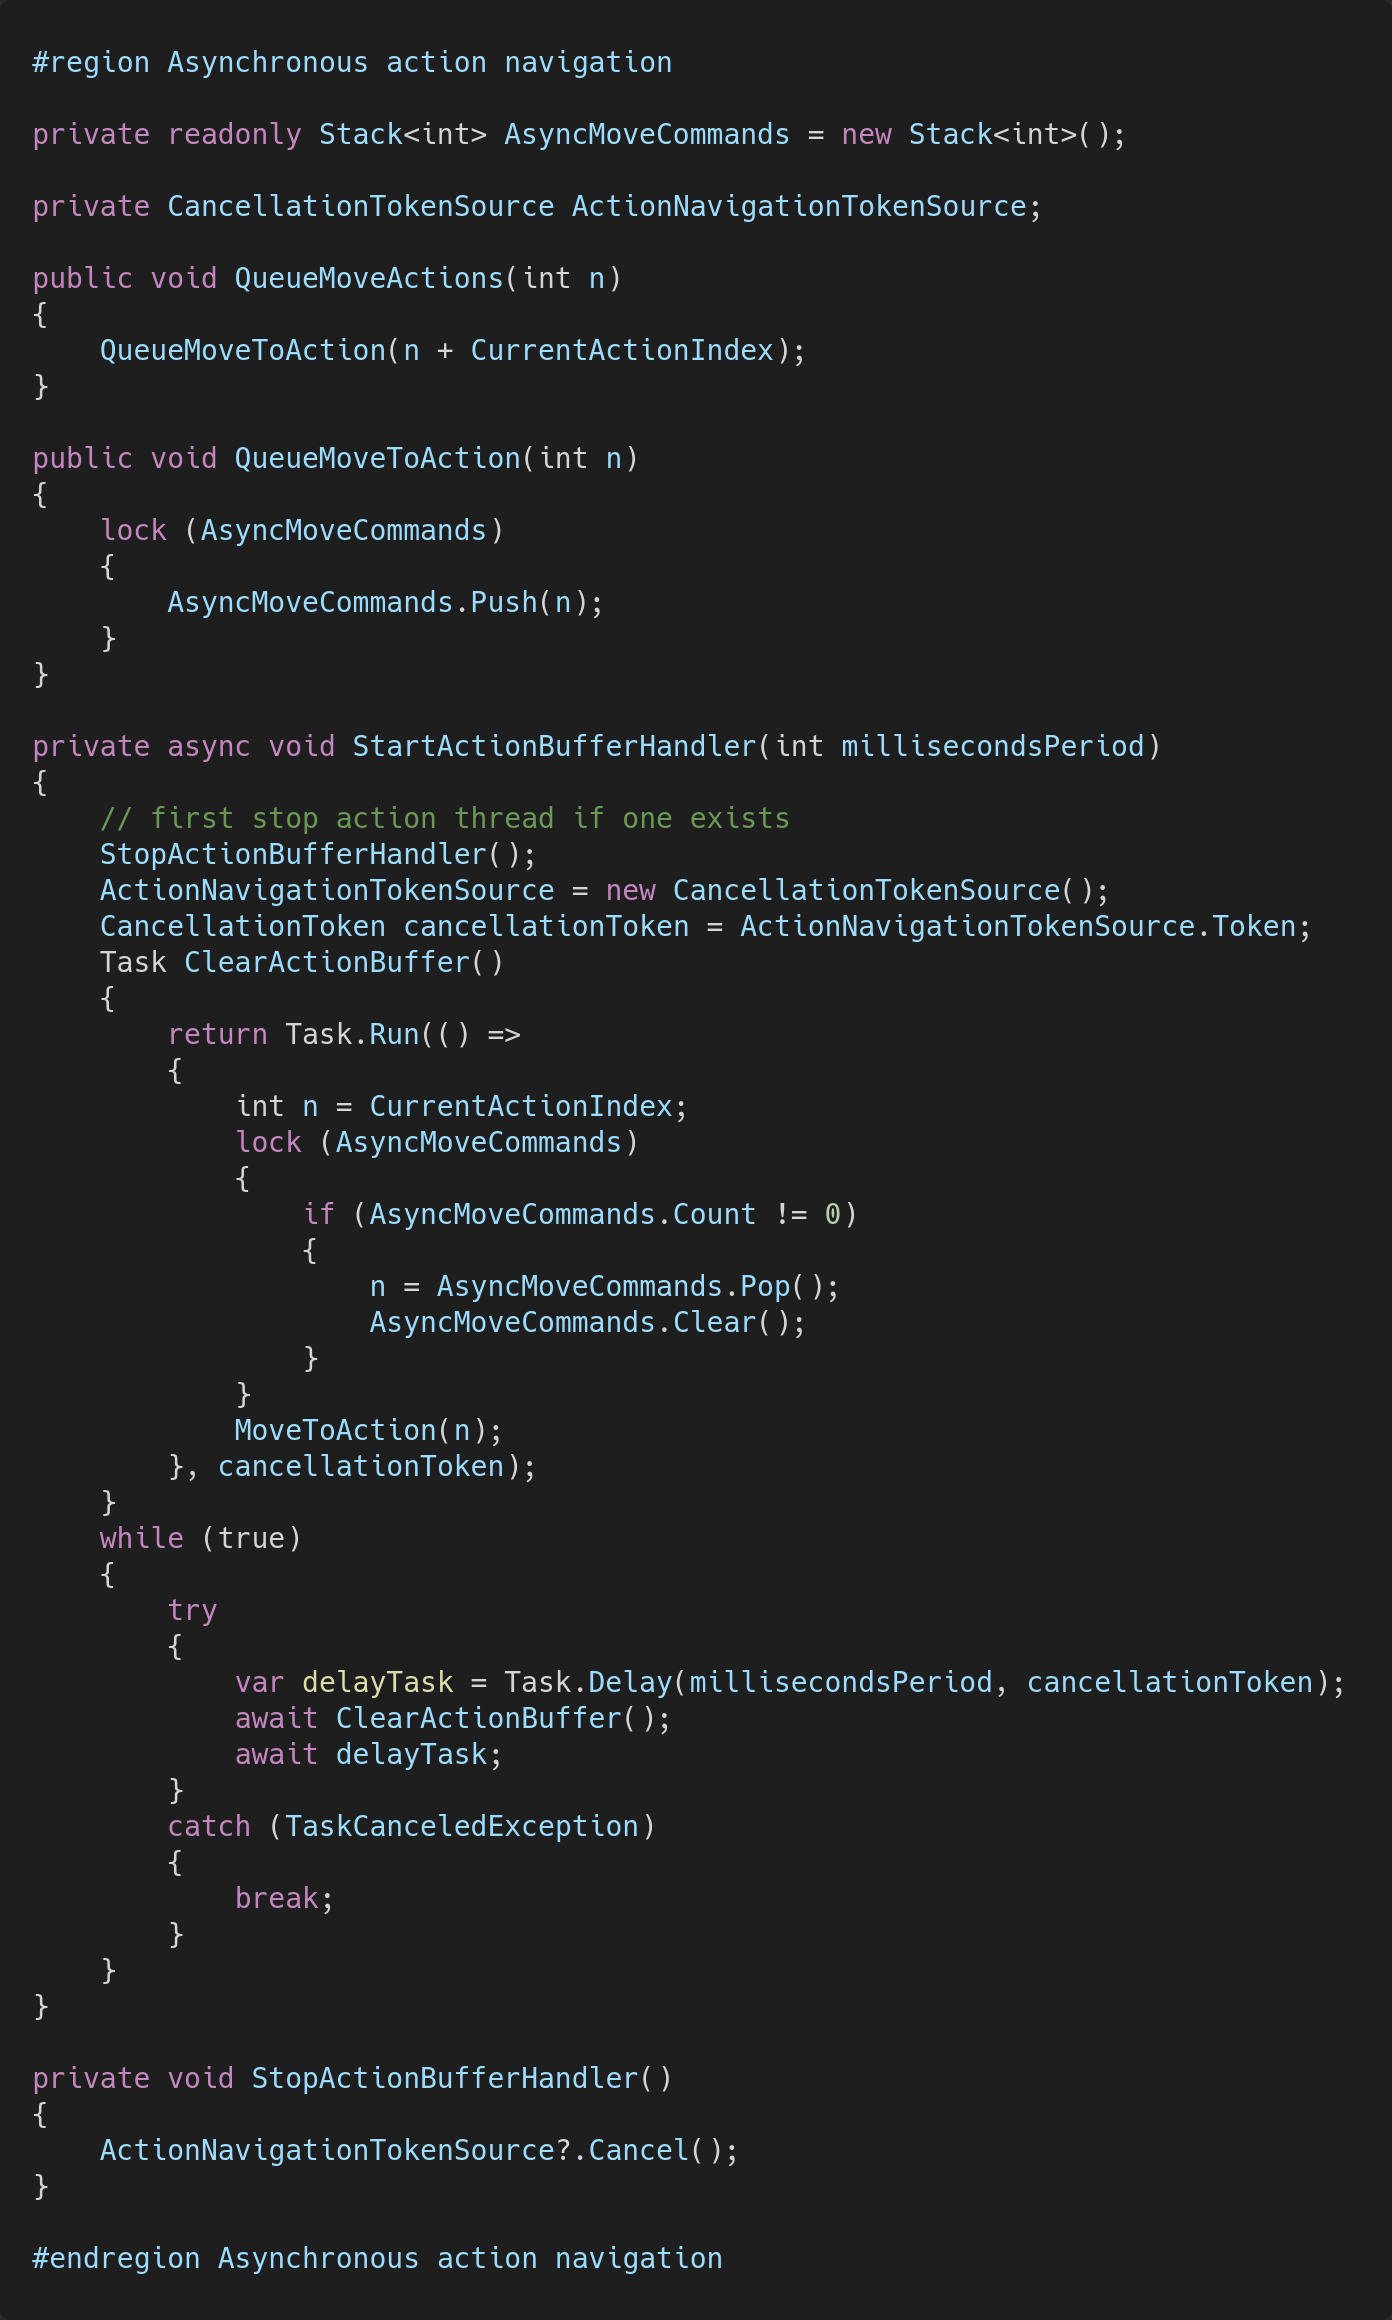
\includegraphics[width=0.85\textwidth]{figures/code/nav-arch/async-navigation.png}
\caption{Asynchronous navigation subsystem}
\label{fig:async.navigation}
\end{figure}

\FloatBarrier

\subsubsection{Centralized navigation system}

While implementing other features such as the diffusion, I noticed that having to implement for each page action the forward and backwards code, my code became quite error-prone. It was hard to notice bugs because it was not feasible to check every single action from both directions manually and creating a testing framework just because of this was out of scope. \\
Some navigation bugs were easy to notice because due to the overall still linear nature of the navigation system, errors did propagate. This means that a error in a previous action most likely did break the page state on future actions because they depend on each other. \\
Nonetheless, this did not help in tracking down the bug because I did not know on which action the error happened. This only further incentivised me to reiterate on the navigation system again.

I summarized all the problems I currently had with my code which not only consisted of performance problems but also with visualization problems. Resizing the window did not appropriately scale the UI elements as can be seen in Figure \ref{fig:plugin.scaling.bug}. Additionally, the current navigation system was quite restricted in what kind of UI elements it supported without further hassle. Since I only updated the existing code during the last time I revisited the navigation system, the core design was still all about directly manipulating and creating UI elements on demand. The functions I wrote revolved around the UI elements I was using thus I could not reuse them if I wanted to use different UI elements; leading to the limited support of the navigation system I mentioned.

\begin{figure}
\begin{subfigure}{\textwidth}
\centering
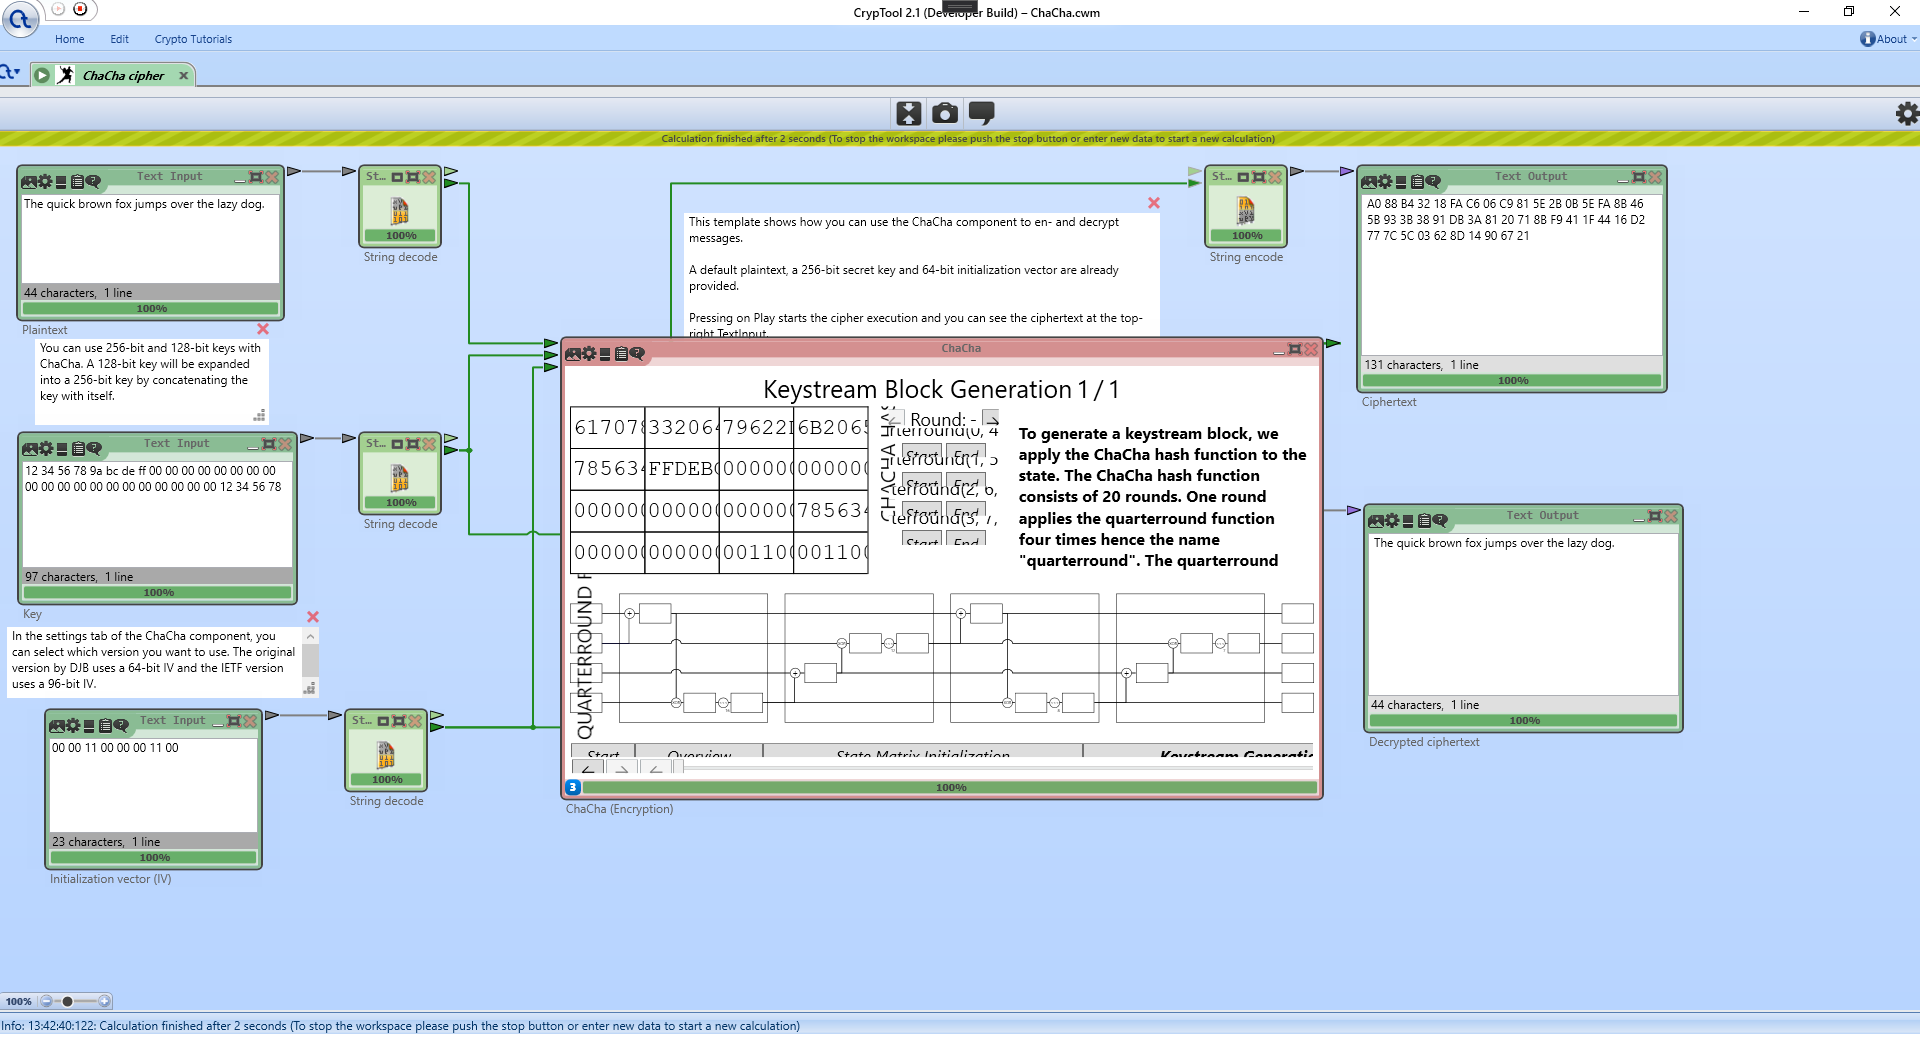
\includegraphics[width=\textwidth]{figures/ct2/scaling-bug-example.png}
\caption{Bad scaling property}
\label{fig:plugin.scaling.bug}
\end{subfigure}
\begin{subfigure}{\textwidth}
\centering
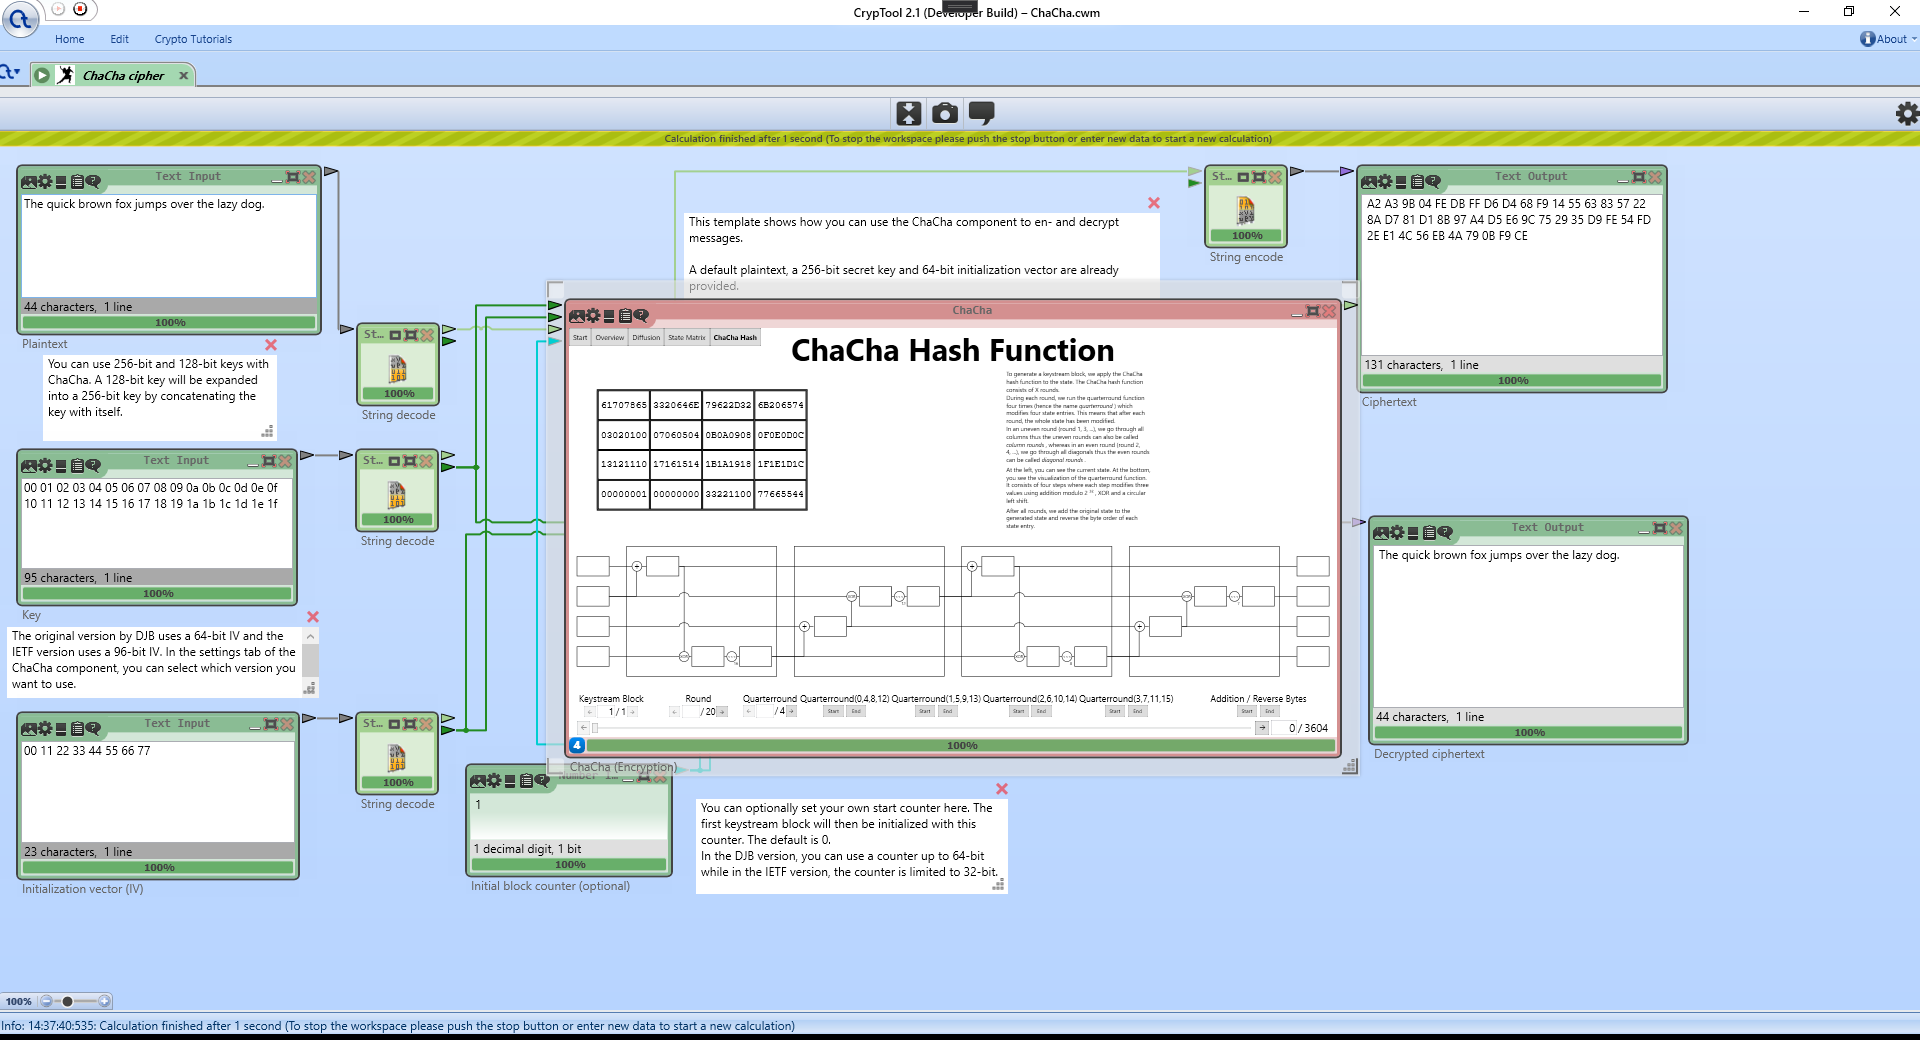
\includegraphics[width=\textwidth]{figures/ct2/scaling-bug-fixed.png}
\caption{Fixed scaling property}
\label{fig:plugin.scaling.fix}
\end{subfigure}
\caption{Example for bad scaling property in previous plug-in versions}
\end{figure}

Essentially, the problem was that I used a lot of code-behind which was highly coupled to the XAML code. I did it like this because it was very straight-forward to do so and lead to fast results. At first, I thought the trade-off between loss of maintainability/flexibility in the future and not having to spend precious time to learn design patterns for WPF applications was worth it. I thought so because I was not writing software on which the long-term success of a company depended and which would get regular updates in the future thus high maintainability or being easy to extend was not a priority. I got proven wrong when I realized I already reached the limit of "code smells" I could handle about one month before I had to hand in my thesis. Every code change kept increasing the accumulated technical debt; killing any motivation I still had left to work on the existing code base. Continuing like this for another month seemed impossible. So I created a list of all current problems together with what requirements a new software architecture would need to meet to solve them:

\begin{description}
\item [(Inconsistent) Performance] The underlying linear design was crippling the performance for the reasons already mentioned. The introduction of caches did only fight the symptoms and not solve the main issue. Further, it made the performance confusing for the users. Sometimes, it took close to no time at all to move to a certain action (action was cached) and on other times, it took quite a lot of time to move to a different action (action was not cached). \\
\textit{\textbf{Requirement}}: Moving to any action should be done in $O(1)$. This means, it should not matter how many actions we needed to skip to arrive at the destination.
\item [Error-prone design for action creation] Writing new actions was error-prone because I needed to write code for forward and backwards navigation which introduced mental overhead because it depended on the code of all previous actions. This also lead to error propagation. Errors were easily noticeable by users but were hard to track down to their origin.\\
\textit{\textbf{Requirement}}: New actions should be able to be written without having to write backwards navigation code. Backwards navigation should be handled automatically and thus be "error-free by design".
\item [No coherent system design] Adding new code without following a design pattern made it hard to grasp the system architecture over the long run. Additionally, the high coupling of the backend (code-behind) with the frontend (XAML) made it harder to implement new features in one part without needing to modify the other part. The system essentially got very rigid and over time, even seemingly small changes took quite some time to implement.\\
\textit{\textbf{Requirement}}: The new system should make it clear what piece of code is responsible for what and thus be highly modular. This should also make it clear where new code must be added to implement a new feature without increasing technical debt; while also decreasing the possibility to introduce bugs since code is less coupled. To summarize, the new architecture should strive for high cohesion, but low coupling.
\end{description}

\begin{figure}[!hbt]
\centering
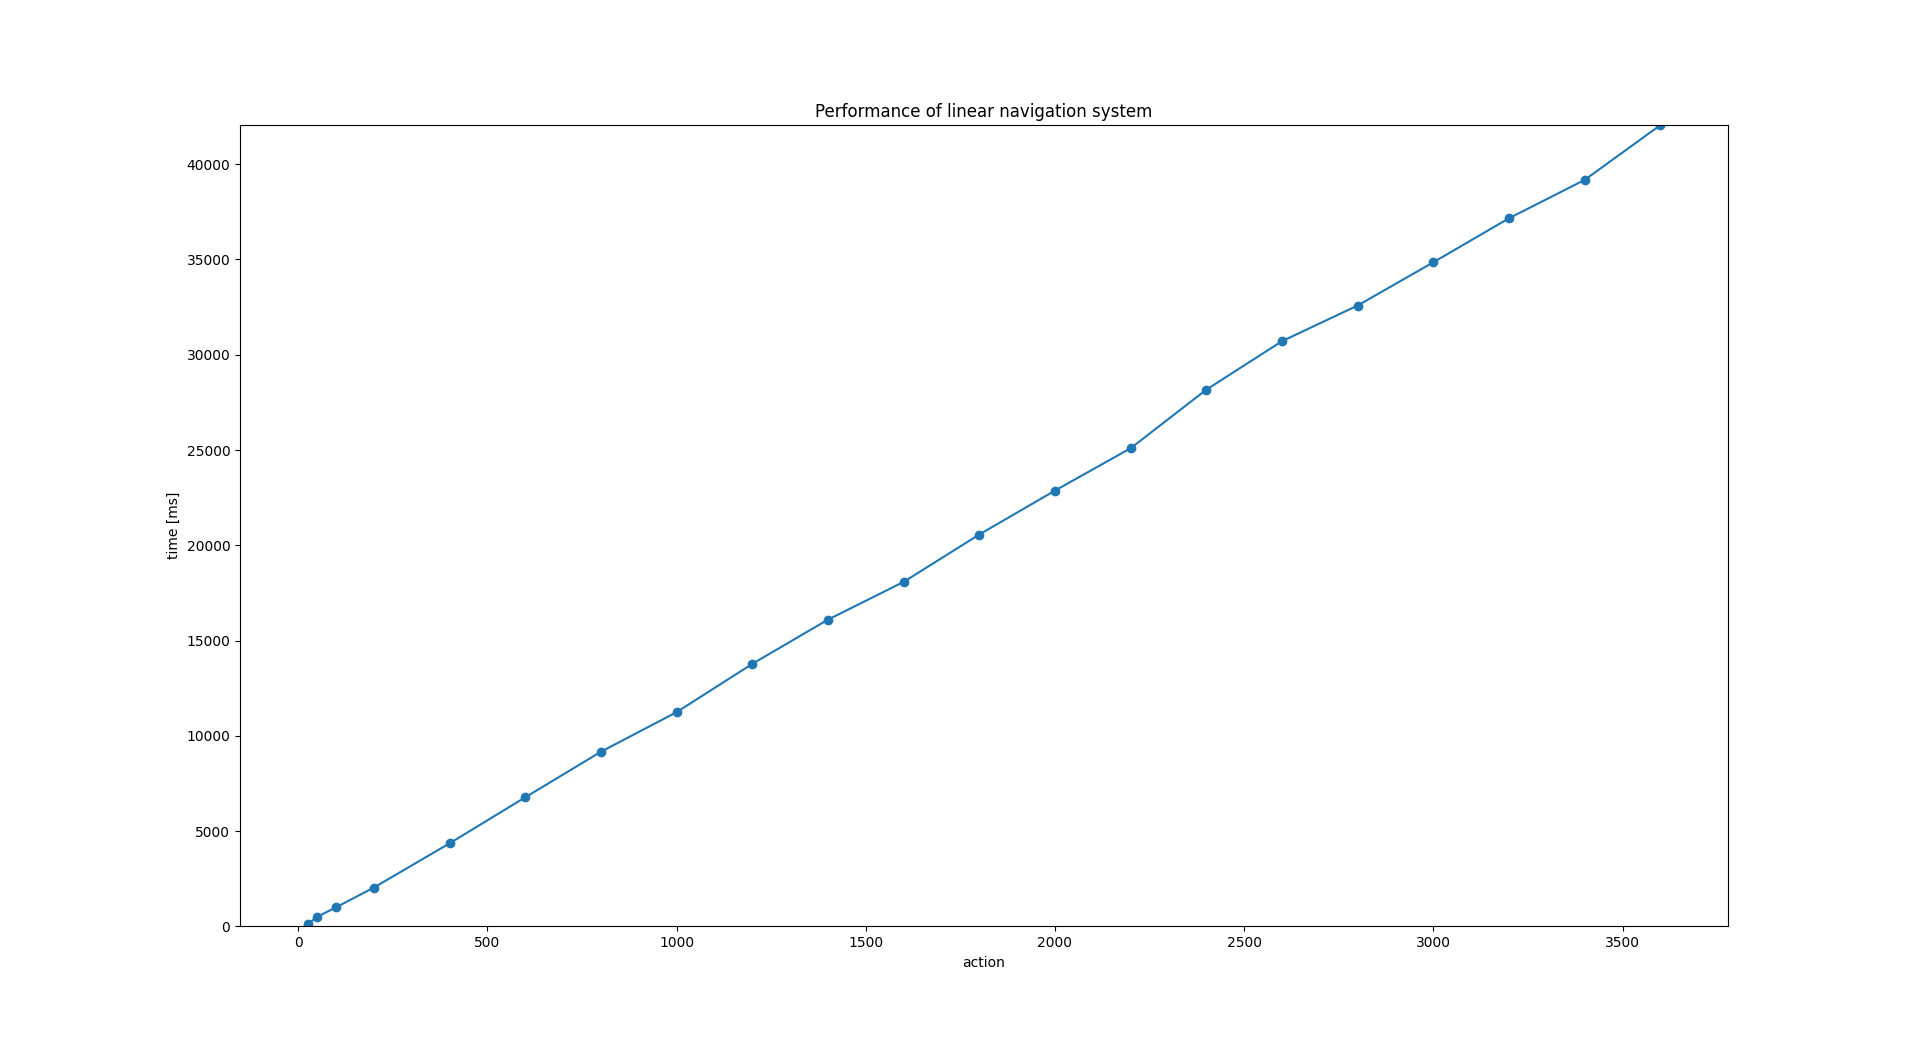
\includegraphics[width=\textwidth]{figures/pyplot/performance_navsystem-linear.png}
\caption{Performance of linear navigation system}
\label{fig:navsystem.performance.linear}
\centering
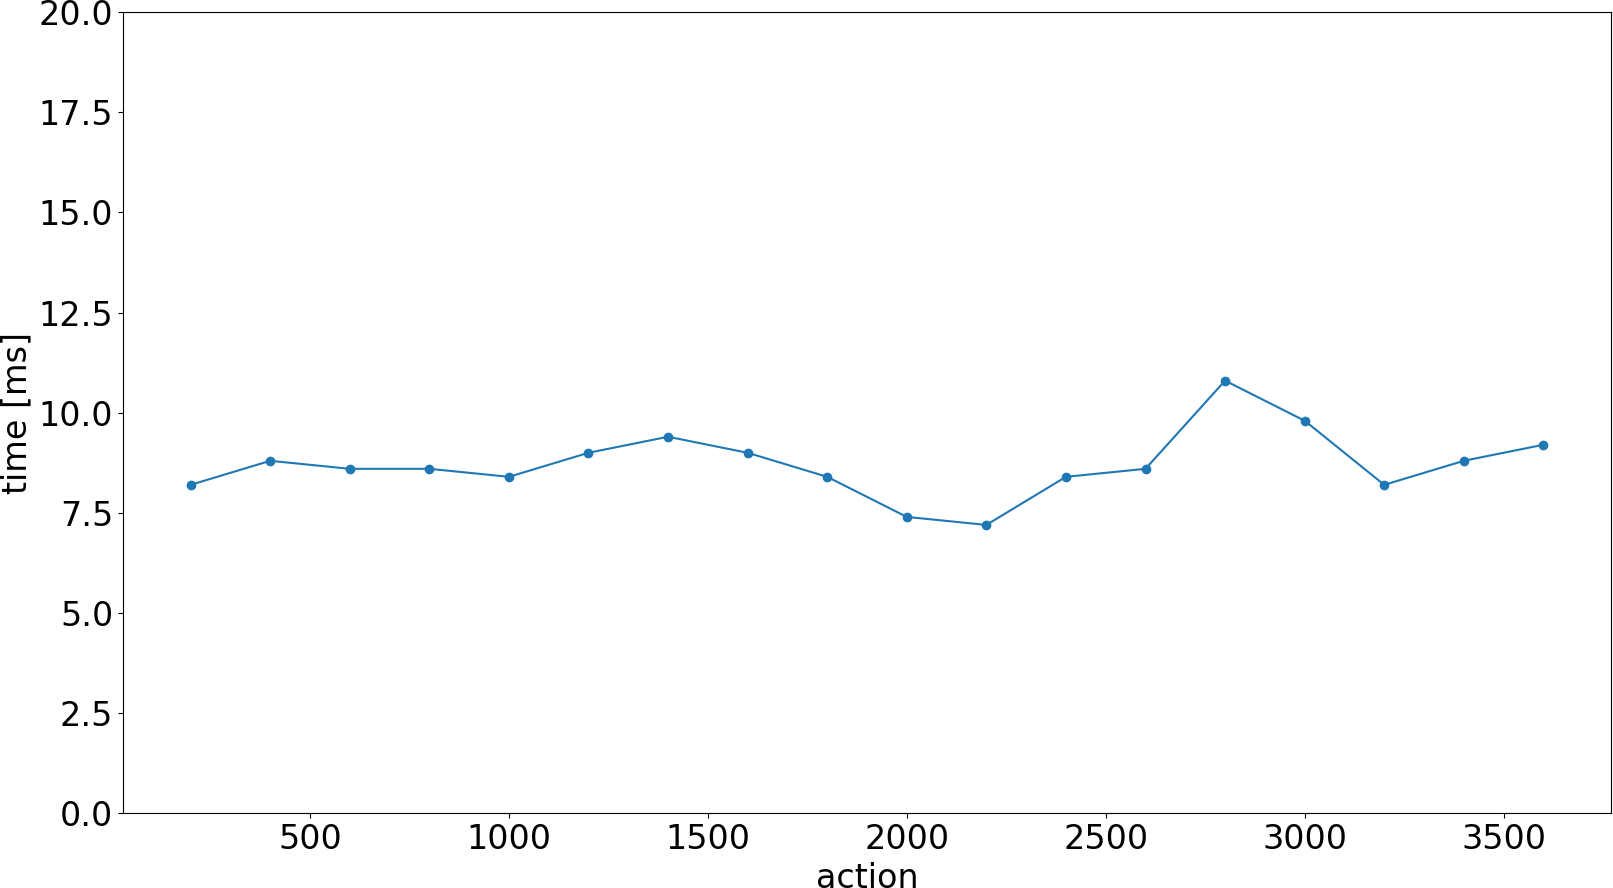
\includegraphics[width=\textwidth]{figures/pyplot/performance_navsystem-central.png}
\caption{Performance of final (centralized) navigation system}
\label{fig:navsystem.performance.central}
\end{figure}

All these problems were solved using the MVVM design pattern with a new navigation system design. To implement them, I completely rewrote the existing code from scratch, which was time-consuming (took about two weeks) but in the end worth it. Figure \ref{fig:navsystem.performance.central} shows the performance of the final navigation system. As one can see, the time it takes to skip actions is constantly very low and only varies between a few milliseconds; making the user interface very responsive.

\begin{figure}
\centering
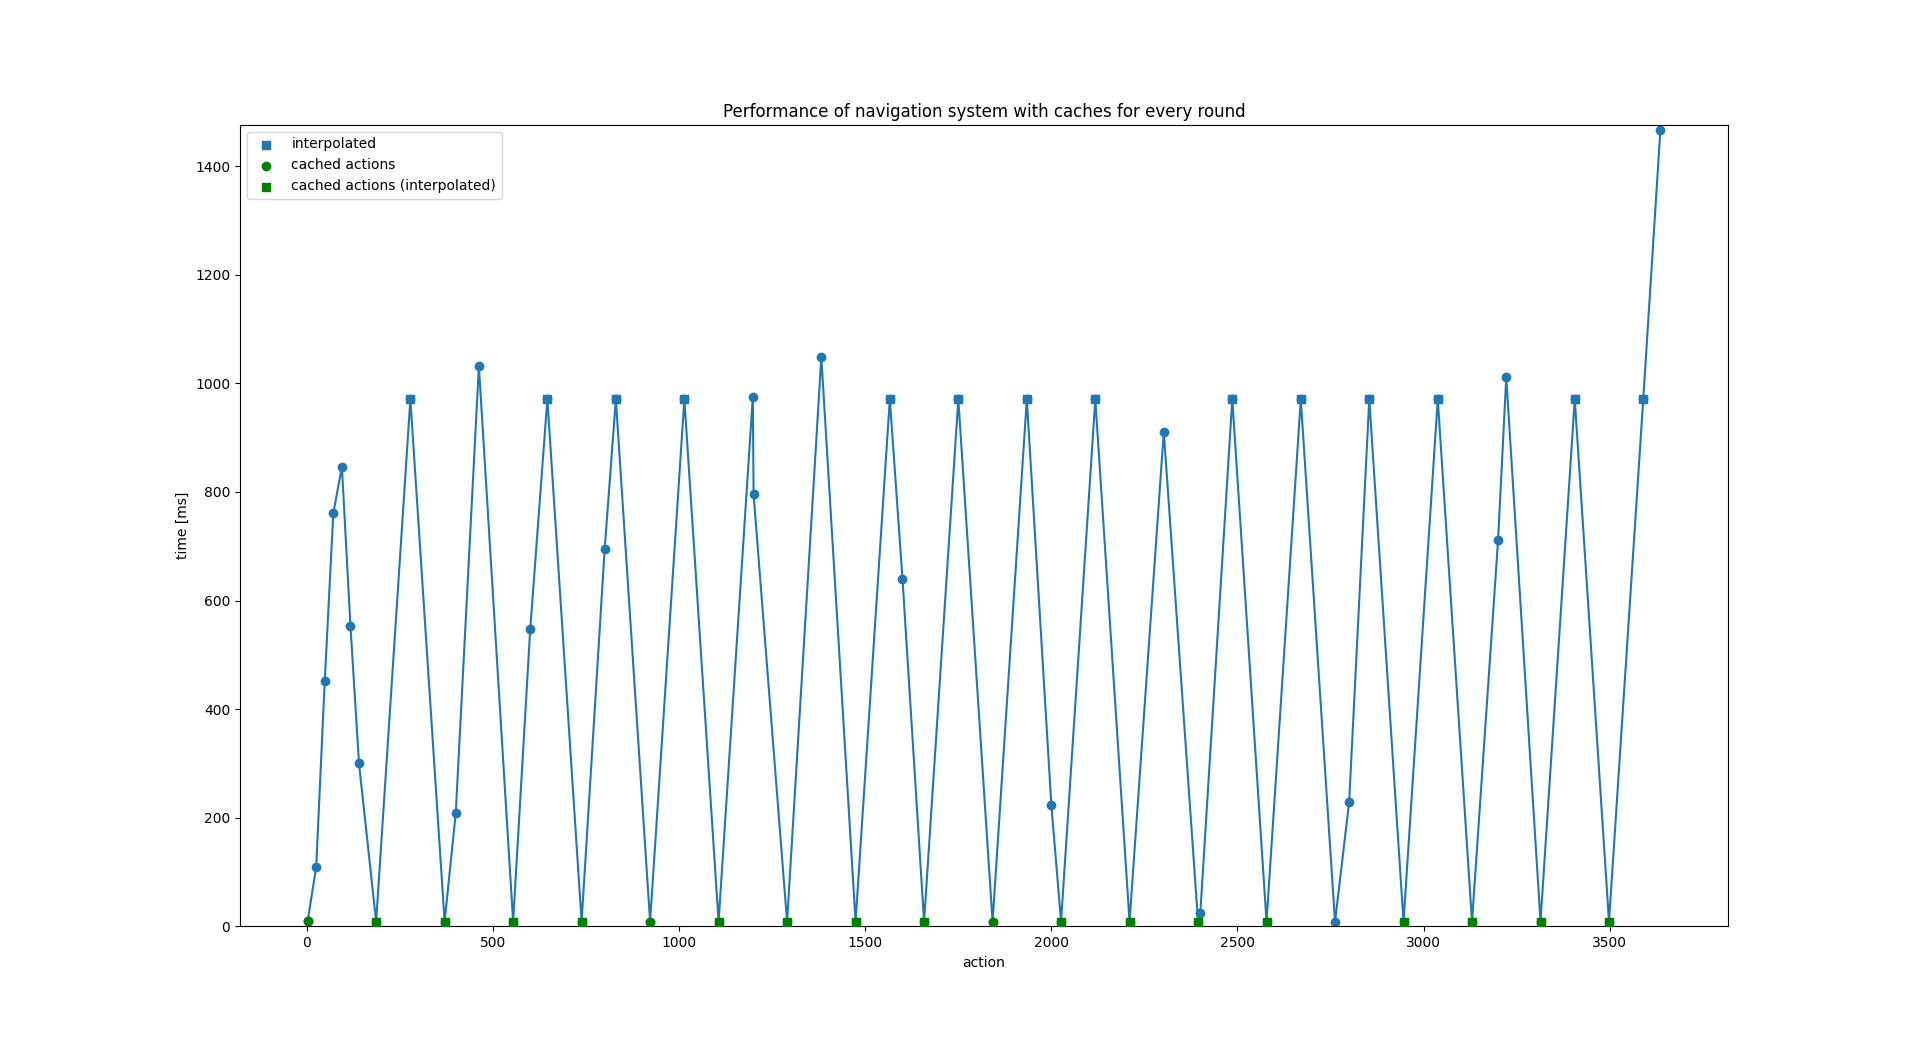
\includegraphics[width=\textwidth]{figures/pyplot/performance_navsystem-round-cache.png}
\caption{Performance of linear navigation system with caches for each round}
\label{fig:navsystem.performance.round}
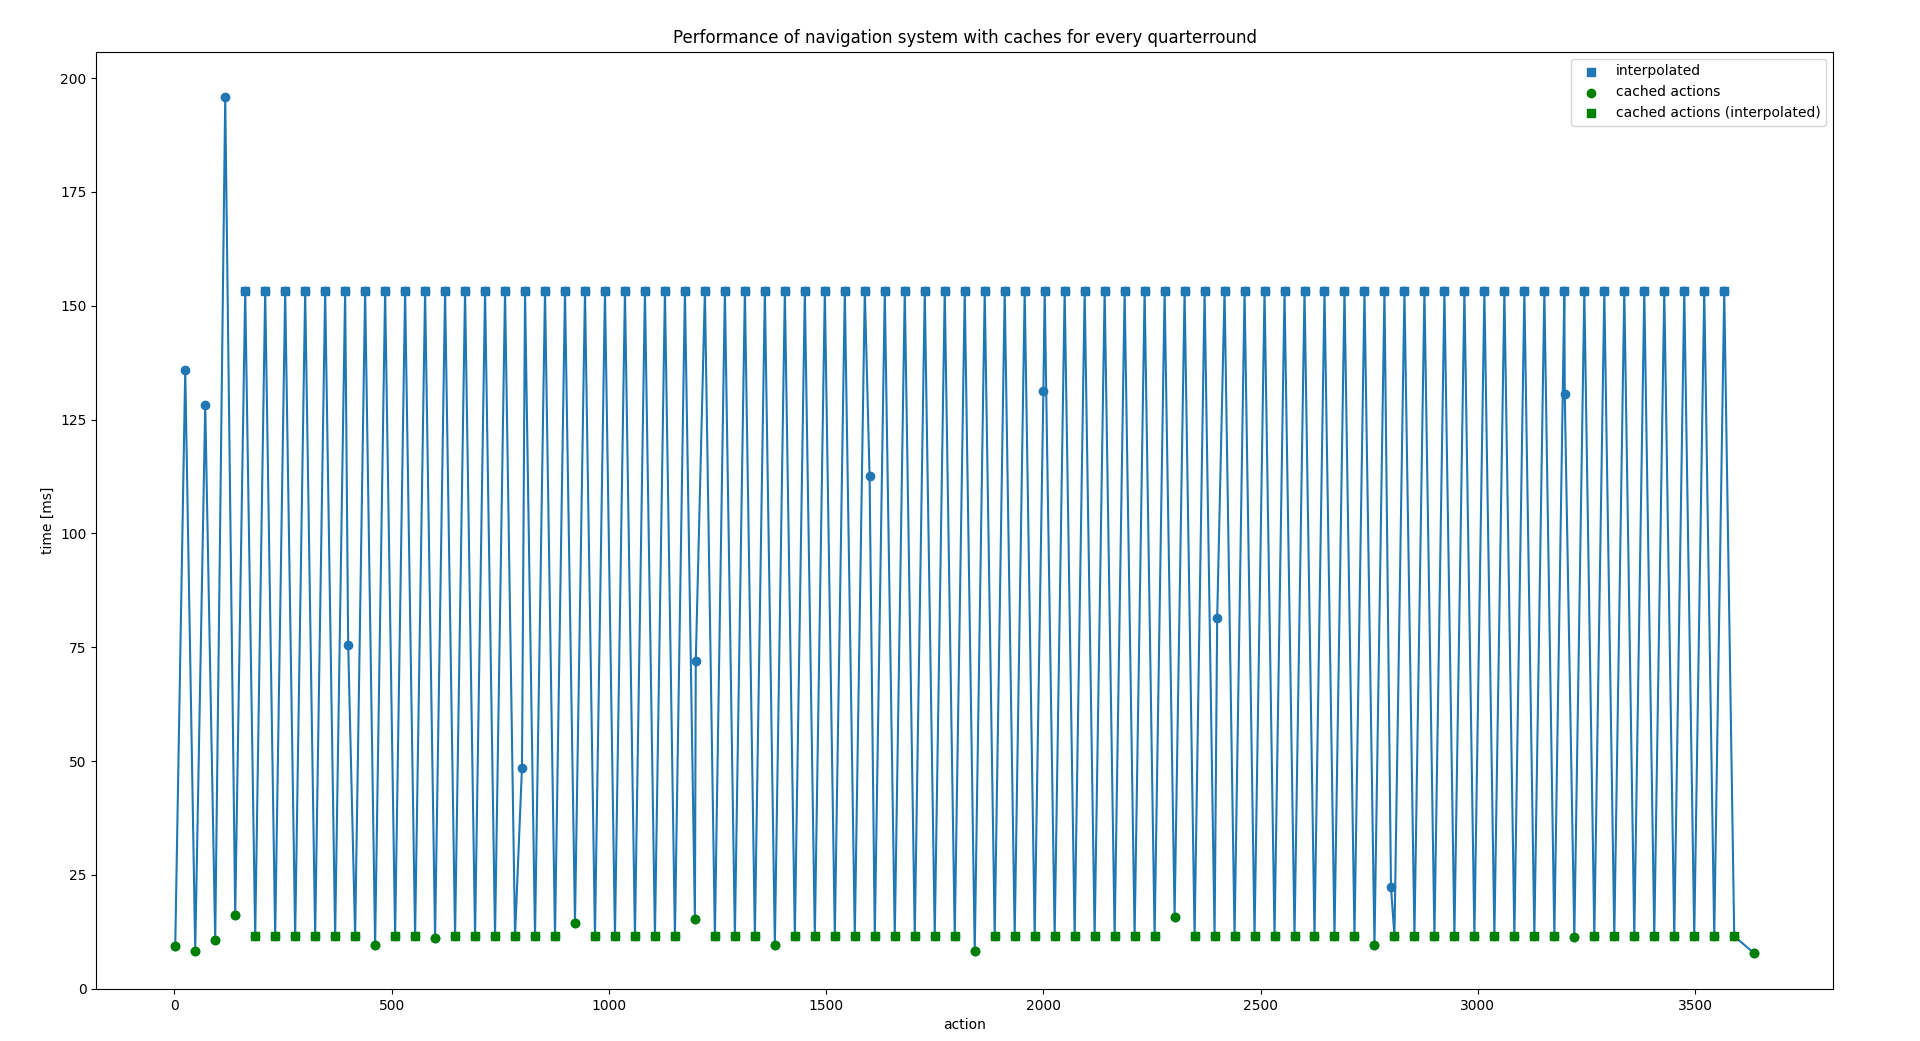
\includegraphics[width=\textwidth]{figures/pyplot/performance_navsystem-qr-cache.png}
\caption{Performance of linear navigation system with caches for each quarter-round}
\label{fig:navsystem.performance.qr}
\end{figure}


%%%%%%%%%%%%%%%%%%%%%%%%%%%%%%%%%%%%%%%%%%%%%%%%%%%%%%%%%%%%%%%%%%%%%%%%
\chapter{Future Work}
\label{chap:futureWork}

In this chapter, I will describe how the plugin could be further improved to make it more useful for the audience of CrypTool 2.

\begin{description}[style=nextline]
\item[Diffusion: XOR input and button to toggle between XOR and actual values] 

Adding a third input to the Diffusion page where the user can explicitly set the XOR of the primary and secondary value would better fit the needs of cryptanalysist who want to study the diffusion property of the cipher since one is more interested in the difference between two values than in their actual values. For example, if we just want to flip one bit, we could just type in a single 1 anywhere into the XOR input. \\
Using the same argument, a button with which one toggle between seeing the XOR of the intermediate values and their actual values during visualization would be useful.

\item[Diffusion: Better overview over flipped bits at the end of each round]

In the Avalanche visualization, at the end of the visualization, I have seen that the author provided a overview over the percentage of flipped bits at the end of each round. I found this very sensible because it shows how the amount of flipped bits goes very fast up to around 50\% and then stays near it which is one would expect from a secure cipher. \\
I have thought about using a plot instead of the simple text which is updated at the end of each round but due to canvas and time constraints, I did not further pursue this idea. I could image to integrate such an overview directly into the Diffusion page. This would need cipher execution while still on the page instead on page exit but this would not be a big problem since a button to start cipher execution would suffice.

\pagebreak

\item[Automatic navigation]

As mentioned in Section \ref{sec:aesVisualization}, in the AES visualization, I have seen a button which lets the visualization run without further user interaction needed. A slider was provided to adjust the speed. I think that such a button could be useful for the ChaCha visualization, too, especially for the page about the ChaCha hash function with its many actions. \\
Since I am already using asynchronous navigation for the action slider (which I think would be needed to let a timer run without blocking the UI), I think implementing this feature could easily be integrated within the existing navigation system. Only page switches could maybe get tricky since the action navigation is handled within each page thus navigating out of a page may not be straight-forward. I have noticed that the automatic navigation in the AES visualization does stop between each step so switching the page automatically may not even be desired.

\item[Salsa20 visualization]

As mentioned in Section \ref{sec:salsaCT2Plugin}, using the now existing codebase for ChaCha visualization to create a Salsa20 visualization would definitely increase the value gained from this thesis. This would at least need adaption of the XAML code for the state matrix initialization and the quarterround since ChaCha and Salsa20 differ in this aspects from each other. It would most likely even increase the value of the ChaCha visualization, since both ciphers could then be compared side-by-side. Since the visualizations would be very similar, comparing them and their diffusion property should be very easy.

\item[Localization and online help]

Currently, most texts are only localized in English. Only the memofields, component labels and plaintext value are also available in German. This should be changed in the near future. Further, there should be an online help for the ChaCha plugin which opens by selecting it and pressing F1.

\end{description}

%%%%%%%%%%%%%%%%%%%%%%%%%%%%%%%%%%%%%%%%%%%%%%%%%%%%%%%%%%%%%%%%%%%%%%%%

% This ensures that the subsequent sections are being included as root
% items in the bookmark structure of your PDF reader.
\bookmarksetup{startatroot}
\backmatter

% \begingroup 
%   \let\clearpage\relax 
%   \glsaddall
%   \printglossary
% \endgroup

\label{sec:index}

\printbibliography

\end{document}